        %%******************************************%%
        %%                                          %%
        %%        Modello di tesi di laurea         %%
        %%            di Andrea Giraldin            %%
        %%                                          %%
        %%             2 novembre 2012              %%
        %%                                          %%
        %%******************************************%%


% I seguenti commenti speciali impostano:
% 1. 
% 2. PDFLaTeX come motore di composizione;
% 3. tesi.tex come documento principale;
% 4. il controllo ortografico italiano per l'editor.

% !TEX encoding = UTF-8
% !TEX TS-program = pdflatex
% !TEX root = tesi.tex
% !TEX spellcheck = it-IT

\documentclass[10pt,                    % corpo del font principale
               a4paper,                 % carta A4
               twoside,                 % impagina per fronte-retro
               openright,               % inizio capitoli a destra
               english,                 
               italian,                 
               ]{book}    

%**************************************************************
% Importazione package
%************************************************************** 

%\usepackage{amsmath,amssymb,amsthm}    % matematica

\usepackage[T1]{fontenc}                % codifica dei font:
                                        % NOTA BENE! richiede una distribuzione *completa* di LaTeX

\usepackage[utf8]{inputenc}             % codifica di input; anche [latin1] va bene
                                        % NOTA BENE! va accordata con le preferenze dell'editor

\usepackage[english, italian]{babel}    % per scrivere in italiano e in inglese;
                                        % l'ultima lingua (l'italiano) risulta predefinita

\usepackage{bookmark}                   % segnalibri

\usepackage{caption}                    % didascalie

\usepackage{chngpage,calc}              % centra il frontespizio

\usepackage{csquotes}                   % gestisce automaticamente i caratteri (")

\usepackage{emptypage}                  % pagine vuote senza testatina e piede di pagina

\usepackage{epigraph}			% per epigrafi

\usepackage{eurosym}                    % simbolo dell'euro

%\usepackage{indentfirst}               % rientra il primo paragrafo di ogni sezione

\usepackage{graphicx}                   % immagini

\usepackage{hyperref}                   % collegamenti ipertestuali

\usepackage[binding=5mm]{layaureo}      % margini ottimizzati per l'A4; rilegatura di 5 mm

\usepackage{listings}                   % codici

\usepackage{microtype}                  % microtipografia

\usepackage{mparhack,fixltx2e,relsize}  % finezze tipografiche

\usepackage{nameref}                    % visualizza nome dei riferimenti                                      

\usepackage[font=small]{quoting}        % citazioni

\usepackage{subfig}                     % sottofigure, sottotabelle

\usepackage[italian]{varioref}          % riferimenti completi della pagina

%\usepackage[dvipsnames]{xcolor}         % colori

\usepackage{booktabs}                   % tabelle                                       
\usepackage{tabularx}                   % tabelle di larghezza prefissata                                    
\usepackage{longtable}                  % tabelle su più pagine                                        
\usepackage{ltxtable}                   % tabelle su più pagine e adattabili in larghezza
\usepackage{etoolbox}
\usepackage{lmodern}
\usepackage[table]{xcolor}
\usepackage{array}
\usepackage{colortbl}
\usepackage{verbatim}
\usepackage[edges]{forest}
\usepackage[explicit]{titlesec}
\usepackage{lipsum}% just to generate text
%*******************Per gestire un'immagine in backgorund*********************************
\usepackage{graphicx}
\usepackage{watermark}
\usepackage{transparent}
%*****************************************************************************************

\usepackage[toc, acronym]{glossaries}   % glossario
                                        % per includerlo nel documento bisogna:
                                        % 1. compilare una prima volta tesi.tex;
                                        % 2. eseguire: makeindex -s tesi.ist -t tesi.glg -o tesi.gls tesi.glo
                                        % 3. eseguire: makeindex -s tesi.ist -t tesi.alg -o tesi.acr tesi.acn
                                        % 4. compilare due volte tesi.tex.

\usepackage[backend=biber,style=verbose-ibid,hyperref,backref]{biblatex}
                                        % eccellente pacchetto per la bibliografia; 
                                        % produce uno stile di citazione autore-anno; 
                                        % lo stile "numeric-comp" produce riferimenti numerici
                                        % per includerlo nel documento bisogna:
                                        % 1. compilare una prima volta tesi.tex;
                                        % 2. eseguire: biber tesi
                                        % 3. compilare ancora tesi.tex.


%**************************************************************
% file contenente le impostazioni della tesi
%**************************************************************

%**************************************************************
% Frontespizio
%**************************************************************

% Autore
\newcommand{\myName}{Federico Perin}                                    
\newcommand{\myTitle}{Il modello Bradley-Terry per l'analisi delle partite della Serie A italiana di calcio}

% Tipo di tesi                   
\newcommand{\myDegree}{Tesi di laurea magistrale}

% Università             
\newcommand{\myUni}{Università degli Studi di Padova}

% Facoltà       
\newcommand{\myFaculty}{Corso di Laurea Magistrale in Informatica}

% Dipartimento
\newcommand{\myDepartment}{Dipartimento di Matematica "Tullio Levi-Civita"}

% Titolo del relatore
\newcommand{\profTitle}{Prof.}

% Relatore
\newcommand{\myProf}{ Annamaria Guolo}

% Luogo
\newcommand{\myLocation}{Padova}

% Anno accademico
\newcommand{\myAA}{2022-2023}

% Data discussione
\newcommand{\myTime}{Febbraio 2023}

\newcommand{\paginavuota}{\newpage\null\thispagestyle{empty}}

\newcommand\textbox[1]{%
	\parbox{.333\textwidth}{#1}%
}

%Numerazione equazione
\newcommand\numberthis{\addtocounter{equation}{1}\tag{\theequation}}

%Argmin
\DeclareMathOperator*{\argminA}{arg\,min} % Jan Hlavacek
\DeclareMathOperator*{\argminB}{argmin}   % Jan Hlavacek
\DeclareMathOperator*{\argminC}{\arg\min}   % rbp

\newcommand{\argminD}{\arg\!\min} % AlfC

\newcommand{\argminE}{\mathop{\mathrm{argmin}}}          % ASdeL
\newcommand{\argminF}{\mathop{\mathrm{argmin}}\limits}   % ASdeL

% limits on side
\DeclareMathOperator{\argminG}{arg\,min} % Jan Hlavacek
\DeclareMathOperator{\argminH}{argmin}   % Jan Hlavacek
\newcommand{\argminI}{\mathop{\mathrm{argmin}}\nolimits} % ASdeL

%Argmax
\DeclareMathOperator*{\argmaxA}{arg\,max} % Jan Hlavacek
\DeclareMathOperator*{\argmaxB}{argmax}   % Jan Hlavacek
\DeclareMathOperator*{\argmaxC}{\arg\max}   % rbp

\newcommand{\argmaxD}{\arg\!\max} % AlfC

\newcommand{\argmaxE}{\mathop{\mathrm{argmax}}}          % ASdeL
\newcommand{\argmaxF}{\mathop{\mathrm{argmax}}\limits}   % ASdeL

% limits on side
\DeclareMathOperator{\argmaxG}{arg\,max} % Jan Hlavacek
\DeclareMathOperator{\argmaxH}{argmax}   % Jan Hlavacek
\newcommand{\argmaxI}{\mathop{\mathrm{argmax}}\nolimits} % ASdeL

\newcommand{\cs}[1]{\texttt{\symbol{`\\}#1}}

\newcommand{\quantities}[1]{%
	\begin{tabular}{@{}c@{}}\strut#1\strut\end{tabular}%
}


%**************************************************************
% Impostazioni di impaginazione
% see: http://wwwcdf.pd.infn.it/AppuntiLinux/a2547.htm
%**************************************************************

\setlength{\parindent}{0pt}   % larghezza rientro della prima riga
\setlength{\parskip}{0pt}   % distanza tra i paragrafi


%**************************************************************
% Impostazioni di biblatex
%**************************************************************

%\begin{comment}
	\bibliography{bibliografia.bib} % database di biblatex 
	
	
	\defbibheading{bibliography} {
		\cleardoublepage
		\phantomsection 
		\addcontentsline{toc}{chapter}{\bibname}
		\chapter*{\bibname\markboth{\bibname}{\bibname}}
	}
	
	\setlength\bibitemsep{1.5\itemsep} % spazio tra entry
	
	\DeclareBibliographyCategory{paper}
	\DeclareBibliographyCategory{web}
	
	\addtocategory{paper}{bradley1952rank}
	\addtocategory{paper}{agresti1992analysis}
	\addtocategory{paper}{tutz1986bradley}
	\addtocategory{paper}{davidson1970extending}
	\addtocategory{paper}{springall1973response}
	\addtocategory{paper}{Turner2012Firth}
	\addtocategory{paper}{francis2010}
	\addtocategory{paper}{schauberger2017}
	\addtocategory{paper}{thurner2000policy}
	\addtocategory{paper}{mauerer2015modeling}
	\addtocategory{paper}{zou2006}
	\addtocategory{paper}{schauberger2019btllasso}
	\addtocategory{paper}{gneiting2007strictly}
	\addtocategory{paper}{R-language}
	\addtocategory{paper}{lago2016home}
	\addtocategory{paper}{cattelan2012models}
	\addtocategory{paper}{tibshirani1996regression}
	\addtocategory{paper}{copas1983regression}
	\addtocategory{paper}{firth2004quasi}
	\addtocategory{paper}{turner2012bradley}
	\addtocategory{paper}{henderson2005bootstrap}
	\addtocategory{paper}{tutz2013visualization}
	\addtocategory{paper}{breiman1996bagging}
	\addtocategory{paper}{freund1996experiments}
	\addtocategory{paper}{dasarathy1991nearest}
	\addtocategory{paper}{GHOLAMI2017515}
	\addtocategory{paper}{charbuty2021classification}
	\addtocategory{paper}{ho1995random}
	\addtocategory{paper}{auer1995gambling}
	\addtocategory{paper}{van2003introduction}
	\addtocategory{paper}{vilela2018towards}
	\addtocategory{paper}{razali2017predicting}
	\addtocategory{paper}{theron2020use}
	\addtocategory{paper}{cattelan2013dynamic}
	\addtocategory{paper}{kang2015poisson}
	\addtocategory{paper}{xu2021prediction}
	
	

	\addtocategory{web}{bt2}
	\addtocategory{web}{storyGenoa}
	\addtocategory{web}{storySal}
	\addtocategory{web}{speculazione}
	\addtocategory{web}{storyAta}
	\addtocategory{web}{storySamp}
	\addtocategory{web}{speculazione}
	\addtocategory{web}{sarrismotr}
	\addtocategory{web}{sarrismo}
	\addtocategory{web}{torino}
	\addtocategory{web}{bet}
	\addtocategory{web}{fbref}
	\addtocategory{web}{serieA}
	\addtocategory{web}{btl}
	\addtocategory{web}{costrdalbasso}
	\addtocategory{web}{minkdist}
	\addtocategory{web}{manhattan}
	\addtocategory{web}{euclidea}
	\addtocategory{web}{kernel}
	\addtocategory{web}{bootstrap}
	\addtocategory{web}{glt}
	\addtocategory{web}{offside}
	\addtocategory{web}{var}
	\addtocategory{web}{rstudio}
	\addtocategory{web}{pycharm}
	\addtocategory{web}{EffectStars2}
	\addtocategory{web}{ggplot2}
	\addtocategory{web}{mltest}
	\addtocategory{web}{sklearn}
	\addtocategory{web}{numpy}
	\addtocategory{web}{matplotlib}
	\addtocategory{web}{pandas}
	\addtocategory{web}{catenaccio}
	

	
	
	\defbibheading{paper}{\section*{Riferimenti bibliografici}}
	\defbibheading{web}{\section*{Siti Web consultati}}
%\end{comment}





%**************************************************************
% Impostazioni di caption
%**************************************************************
\captionsetup{
	tableposition=top,
	figureposition=bottom,
	font=small,
	format=hang,
	labelfont=bf
}

%**************************************************************
% Impostazioni di glossaries
%**************************************************************
\makeglossaries

%**************************************************************
% Acronimi
%**************************************************************
\renewcommand{\acronymname}{Acronimi e abbreviazioni}

\newacronym[description={\glslink{apig}{\textit{Application Program Interface}}}]
    {api}{API}{Application Program Interface}
    
\newacronym[description={\textit{Advanced Workforce Management System}}]
	{AWMS}{AWMS}{Advanced Workforce Management System}

\newacronym[description={\glslink{umlg}{\textit{Unified Modeling Language}}}]
    {uml}{UML}{Unified Modeling Language}
    
\newacronym[description={\textit{Test End to End}}]
	{test e2e}{E2E}{test End to End}

\newacronym[description={\textit{Internazionalizzazione}}]
	{i18n}{i18n}{internazionalizzazione}

\newacronym[description={\glslink{JSONg}{\textit{JavaScript Object Notation}}}]
	{JSON}{JSON}{JavaScript Object Notation}
	
\newacronym[description={\glslink{restg}{\textit{Representational State Transfer}}}]
	{rest}{REST}{Representational State Transfer}	

\newacronym[description={\glslink{httpg}{\textit{Hyper Text Transfer Protocol}}}]
{http}{HTTP}{Hyper Text Transfer Protocol}	
	
\newacronym[description={\textit{Hyper Text Markup Language}}]
	{HTML}{HTML}{HyperText Markup Language}	
	
\newacronym[description={\textit{Cascading Style Sheets}}]
	{CSS}{CSS}{Cascading Style Sheets}
	
\newacronym[description={\textit{Syntactically Awesome StyleSheets}}]
	{Sass}{Sass}{Syntactically Awesome StyleSheets}
	
\newacronym[description={\textit{Hypertext Preprocessor}}]
	{PHP}{PHP}{Hypertext Preprocessor}	
	
\newacronym[description={\glslink{urlg}{\textit{Uniform Resource Locator}}}]
	{url}{URL}{Uniform Resource Locator}	
			
\newacronym[description={\glslink{httpsg}{\textit{Hyper Text Transfer Protocol over Secure Socket Layer}}}]
	{https}{HTTPS}{Hyper Text Transfer Protocol over Secure Socket Layer}	
		
\newacronym[description={\glslink{dbmsg}{\textit{Database Management System}}}]
	{DBMS}{DBMS}{Database Management System}

\newacronym[description={\glslink{domg}{\textit{Document Object Model}}}]
	{DOM}{DOM}{Document Object Model}

\newacronym[description={\textit{World Wide Web Consortium}}]
	{W3C}{W3C}{World Wide Web Consortium}

\newacronym[description={\glslink{gdprg}{\textit{General Data Protection Regulation}}}]
	{GDPR}{GDPR}{General Data Protection Regulation}	

\newacronym[description={\glslink{sdkg}{\textit{Software Development Kit}}}]
	{sdk}{SDK}{Software Development Kit}

\newacronym[description={\textit{eXtensible Markup Language}}]
	{XML}{XML}{eXtensible Markup Language}	

\newacronym[description={\textit{eXtensible Hyper Text Markup Language}}]
	{XHTML}{XHTML}{eXtensible Hyper Text Markup Language}
	
\newacronym[description={\textit{behavior-driven development}}]
	{BDD}{BDD}{behavior-driven development}
%**************************************************************
% Glossario
%**************************************************************
\renewcommand{\glossaryname}{Glossario}

\newglossaryentry{apig}
{
	name=\glslink{api}{\textit{API}},
	text=Application Program Interface,
	sort=api,
	description={In informatica con il termine \emph{Application Programming Interface (API)} (ing. interfaccia di programmazione di un'applicazione) si indica ogni insieme di procedure disponibili al programmatore, di solito raggruppate a formare un set di strumenti specifici per l'espletamento di un determinato compito all'interno di un certo programma. La finalità è ottenere un'astrazione, di solito tra l'\emph{hardware} e il programmatore o tra \emph{software} a basso e quello ad alto livello semplificando così il lavoro di programmazione}
}

\newglossaryentry{umlg}
{
	name=\glslink{uml}{\textit{UML}},
	text=UML,
	sort=uml,
	description={in ingegneria del software \emph{UML, Unified Modeling Language} (ing. linguaggio di modellazione unificato) è un linguaggio di modellazione e specifica basato sul paradigma object-oriented. L'\emph{UML} svolge un'importantissima funzione di ``lingua franca'' nella comunità della progettazione e programmazione a oggetti. Gran parte della letteratura di settore usa tale linguaggio per descrivere soluzioni analitiche e progettuali in modo sintetico e comprensibile a un vasto pubblico}
}

\newglossaryentry{Electrolux}
{
	name={\textit{Electrolux}},
	text=Electrolux,
	sort=electrolux,
	description={Electrolux è una multinazionale svedese produttrice di elettrodomestici con sede a Stoccolma}
}

\newglossaryentry{machine learning}
{
	name={\textit{Machine learning}},
	text=machine learning,
	sort=machine learning,
	description={Nell'ambito dell'informatica, (ing.apprendimento automatico) l'apprendimento automatico è una variante alla programmazione tradizionale nella quale in una macchina si predispone l'abilità di apprendere qualcosa dai dati in maniera autonoma, senza istruzioni esplicite}
}

\newglossaryentry{plant manager}
{
	name={\textit{Plant manager}},
	text=plant manager,
	sort=plant manager,
	description={È colui (ing.responsabile di stabilimento) che presiede e organizza le operazioni quotidiane degli impianti di produzione aziendali, di cui deve assicurare il funzionamento ottimale ed efficiente. Si occupa dei lavoratori, assegnando funzioni e ruoli, definendo orari di lavoro e produzione. Raccoglie e analizza i dati di produzione per trovare eventuali spazi di miglioramento. Si occupa della sicurezza dei lavoratori e quella degli impianti inoltre, monitora le apparecchiature di produzione e, in caso di necessità, della loro riparazione o sostituzione}
}

\newglossaryentry{bot}
{
	name={\textit{Bot}},
	text=bot,
	sort=bot,
	description={È un \emph{software} progettato per simulare una conversazione con un essere umano. Lo scopo principale di questi \emph{software} è quello di simulare un comportamento umano e sono a volte definiti anche agenti intelligenti e vengono usati per vari scopi come la guida in linea, per rispondere alle FAQ degli utenti che accedono a un sito. In alcuni utilizzano sofisticati sistemi di elaborazione del linguaggio naturale, ma molti si limitano a eseguire la scansione delle parole chiave nella finestra di input e fornire una risposta con le parole chiave più corrispondenti}
}

\newglossaryentry{QR code}
{
	name={\textit{QR code}},
	text=QR code,
	sort=qr-code,
	description={È un codice a barre bidimensionale (o codice 2D), ossia a matrice, composto da moduli neri disposti all'interno di uno schema bianco di forma quadrata, impiegato tipicamente per memorizzare informazioni generalmente destinate a essere lette tramite uno \emph{smartphone}}
}

\newglossaryentry{WebSocket}
{
	name={\textit{WebSocket}},
	text=WebSocket,
	sort=websocket,
	description={È una tecnologia web che fornisce canali di comunicazione a due direzioni cioè gli interlecutori possono sia inviare sia ricevere contemporaneamente attraverso una singola connessione TCP}
}

\newglossaryentry{SCRUM}
{
	name={\textit{SCRUM}},
	text=SCRUM,
	sort=scrum,
	description={È un \emph{framework} agile per la gestione del ciclo di sviluppo del \emph{software}, iterativo ed incrementale, concepito per gestire progetti e prodotti software o applicazioni di sviluppo. Nel proprio manifesto prevede i seguenti punti che lo caratterizzano, le persone e le interazioni sono più importanti dei processi e degli strumenti, meglio avere da subito \emph{software} funzionante che documentazione ampia, meglio una collaborazione con il cliente piuttosto che fare una negoziazione del contratto, essere in grando di rispondere ai cambiamenti piuttosto che rispettare un piano. 
		I progetti Scrum progrediscono attraverso una serie di sprint che hanno una durata massima di un mese. Negli sprint vengono decisi quali requisiti devono essere soddisfatti, e quindi successivamente, progettati, implementati e testati}
}

\newglossaryentry{framework}{
	name={\textit{Framework}},
	text=framework,
	sort=framework,
	description={In informatica con il termine framework 
		si indica un insieme di elementi \emph{software} che un programmatore può usare o modificare per realizzare un programma. Rappresenta un’astrazione composta da elementi universali e riutilizzabili con lo scopo di facilitare lo sviluppo di un programma e di far applicare buone norme di programmazione. Inoltre, un framework può offrire programmi di supporto, librerie, compilatori e documentazione per l'utilizzo}
}

\newglossaryentry{iOS}{
	name={\textit{iOS}},
	text=iOS,
	sort=iOS,
	description={È un sistema operativo \emph{mobile} sviluppato da Apple per iPhone, iPod touch e iPad. Le versioni principali di iOS vengono distribuite ogni anno. L'attuale versione, iOS 13, è stata distribuita al pubblico il 19 settembre 2019}
}

\newglossaryentry{Android}{
	name={\textit{Android}},
	text=Android,
	sort=Android,
	description={È un sistema operativo per dispositivi \emph{mobile} sviluppato da Google e basato sul kernel Linux, progettato principalmente per \emph{smartphone} e \emph{tablet}, interfacce utente specializzate per televisori (Android TV), automobili (Android Auto), orologi da polso (Wear OS), occhiali (Google Glass). L'attuale ultima versione è Android 11}
}

\newglossaryentry{architettura}{
	name={\textit{Architettura}},
	text=architettura,
	sort=architettura,
	description={In informatica con il termine architettura, in questo caso intesa come architettura \emph{software}, è l'organizzazione fondamentale di un sistema, definita dai suoi componenti, dalle relazioni reciproche tra i componenti e con l'ambiente, e i principi che ne governano la progettazione e l'evoluzione}
}

\newglossaryentry{linguaggio di markup}{
	name={\textit{Linguaggio di markup}},
	text=linguaggio di markup,
	sort=linguaggio di markup,
	description={In informatica con il termine linguaggio di markup, si intende un gruppo di regole detti marcatori, attraverso le quali vengono descritti i meccanismi di rappresentazione di un testo}
}

\newglossaryentry{browser web}{
	name={\textit{Browser web}},
	text=browser web,
	sort=browser web,
	description={In informatica si intende un'applicazione per l'acquisizione, la presentazione e la navigazione di risorse sul web. Permette la visualizzazione dei contenuti ipertestuali, e la riproduzione di contenuti multimediali. Tra i browser più popolari vi sono Google Chrome, Internet Explorer, Mozilla Firefox, Microsoft Edge, Safari, Opera}
}

\newglossaryentry{applicazione nativa}{
	name={\textit{Applicazione nativa}},
	text=applicazione nativa,
	sort=applicazione nativa,
	description={In informatica si intende un'applicazione scritta e compilata per una specifica piattaforma utilizzando i linguaggi di programmazione e librerie supportati dal particolare sistema operativo \emph{mobile}}
}

\newglossaryentry{applicazione web mobile}{
	name={\textit{Applicazione web mobile}},
	text=applicazione web mobile,
	sort=applicazione web mobile,
	description={In informatica si intende pagine web ottimizzate per dispositivi \emph{mobile} scritte utilizzando tecnologie web, in particolare \gls{HTML}, JavaScript e \gls{CSS}. Inoltre, le applicazioni web non possono accedere alle funzionalità del dispositivo ad'esempio la fotocamera}
}

\newglossaryentry{applicazione ibrida}{ %va a benzina ma anche con l'elettricità
	name={\textit{Applicazione ibrida}},
	text=applicazione ibrida,
	sort=applicazione ibrida,
	description={In informatica si intende applicazioni sviluppate con tecnologie web e vengono eseguite localmente all’interno di un’applicazione nativa. Grazie a ciò possono interagire con il dispositivo ad'esempio utilizzare la fotocamera}
}

\newglossaryentry{notifica push}{ 
	name={\textit{Notifica push}},
	text=notifica push,
	sort=notifica push,
	description={In informatica si intende un tipo di messaggistica istantanea grazie alla quale il messaggio perviene al destinatario senza che questo debba effettuare un'operazione di scaricamento. Tale modalità è quella tipicamente usata da applicazioni come \emph{WhatsApp} o da servizi di sistemi operativi come \g{Android}, oppure da numerose applicazioni derivate da siti web come, ad esempio, il servizio meteo o quello delle notizie}
}

\newglossaryentry{licenza MIT}{ 
	name={\textit{Licenza MIT}},
	text=licenza MIT,
	sort=licenza MIT,
	description={La Licenza MIT è una licenza di \emph{software} libero. È una licenza permissiva, cioè permette il riutilizzo nel \emph{software} proprietario sotto la condizione che la licenza sia distribuita con tale \emph{software}}
}

\newglossaryentry{JSONg}{ 
	name=\glslink{JSON}{\textit{JSON}},
	text=JavaScript Object Notation,
	sort=JSON,
	description={In informatica con il termine \emph{JavaScript Object Notation (JSON)}(ing.Notazione degli oggetti JavaScript) si intende un formato testuale standard, usato per rappresentare dati strutturati basati sulla sintassi degli oggetti in JavaScript. È comunemente utilizzato per l'interscambio di dati fra applicazioni client/server. Risulta essere facile da comprendere e da scrivere per le persone mentre per le macchine risulta essere un formato leggero e veloce da analizzare}
}

\newglossaryentry{pooling}{ 
	name={\textit{Pooling}},
	text=pooling,
	sort=pooling,
	description={In informatica con il termine pooling si intende una procedura attraverso la quale periodicamente viene eseguita una operazione. Nel caso delle comunicazioni tra \g{client} e \g{server} il pooling è la richiesta periodica del \g{client} di dati al \g{server} per controllare sei i dati che ha sono aggiornati}
}

\newglossaryentry{client}{ 
	name={\textit{Client}},
	text=client,
	sort=client,
	description={In informatica con il termine client si intende un entita presente in un rete di comunicazione che accede ai servizi o alle risorse messe a dispozione da un'altra componente detta \g{server}, la cui comunicazione tra client e \g{server} è regolata da insieme di regole e norme detti protocolli di comunicazione. Insieme al \g{server} forma l'architettura client/server}
}

\newglossaryentry{server}{ 
	name={\textit{Server}},
	text=server,
	sort=server,
	description={In informatica con il termine client si intende un entita presente in un rete di comunicazione che offre dei servizi o dalle risorse a un'altri componenti presenti nella rete detti \g{client}, la cui comunicazione tra \g{client} e server è regolata da insieme di regole e norme detti protocolli di comunicazione. Insieme al \g{client} forma l'architettura client/server}
}

\newglossaryentry{httpg}{ 
	name=\glslink{http}{\textit{HTTP}},
	text=Hyper Text Transfer Protocol,
	sort=http,
	description={In informatica con il termine \emph{Hyper Text Transfer Protocol (HTTP)} (ing. protocollo di trasferimento di un ipertesto) si intende un insieme di regole e norme che regolano la trasmissione e la comunicazione d'informazione nella rete Internet. Questo trasmissione d'informazioni avviene sotto forma di scambi di messaggi tipicamente tra il client che puo essere un \g{browser web}, e un server}
}

\newglossaryentry{open-source}{ 
	name={\textit{Open-source}},
	text=open-source,
	sort=open-source,
	description={In informatica con il termine open-source (ing. sorgente libero) si intende un \emph{software} per cui chi lo ha sviluppato rinuncia alla propretà del \emph{software} dando libero accesso a tutto il codice sorgente a chiunque, e quindi è permesso a tutti di contribuire nello sviluppo del codice al fine di migliorarlo, aggiungere nuove funzionalità o  correggere errori all'interno del codice}
}

\newglossaryentry{restg}{ 
	name=\glslink{rest}{\textit{REST}},
	text=Representational State Transfer,
	sort=rest,
	description={In informatica con il termine \emph{Representational State Transfer (REST)} (ing. trasferimento di stato rappresentativo) si intende un approccio architetturale alla creazione di web \g{api} basato sul protocollo di comunicazione \g{http}. Viene imposto che le \g{api} devono permettere di accedere a delle risorse attraverso un \g{url}, utilizzare il formato \gls{JSON} e \gls{XML}, non avere uno stato cioè non deve essere memorizzato cioè che è stato fatto e infine, utilizzare i metodi del \g{http}, GET, POST, PUT, DELETE}
}

\newglossaryentry{urlg}{ 
	name=\glslink{url}{\textit{URL}},
	text=Uniform Resource Locator,
	sort=url,
	description={In informatica con il termine \emph{Uniform Resource Locator (URL)} (ing. localizzare di risorse uniformi) in intede una sequenza di caratteri che identifica univocamente l'indirizzo di una risorsa su una rete di computer, come ad esempio un documento, un'immagine, un video, tipicamente presente su un \g{server} e resa accessibile a un \g{client}}
}

\newglossaryentry{front-end}{ 
	name={\textit{Front-end}},
	text=front-end,
	sort=front-end,
	description={In informatica con il termine front-end si intende la parte visibile all'utente di un programma e con cui egli può interagire solitamente è un'interfaccia utente. Perciò il front-end è la parte di un sistema \emph{software} che gestisce l'interazione con l'utente, ricevendo da esso un input da cui viene prodotto (dal \g{back-end}) un output da mostrare all'utente}
}

\newglossaryentry{back-end}{ 
	name={\textit{Back-end}},
	text=back-end,
	sort=back-end,
	description={In informatica con il termine back-end si intende la parte che si occuppa di ricevere in input dati inseriti dall'utenti e di eleborarli per rispondere alle richieste dell'utente. Dopo l'elaborazione dei dati il back-end produce un risultato che sarà compito del \g{front-end} mostrarlo}
}

\newglossaryentry{httpsg}{ 
	name=\glslink{https}{\textit{HTTPS}},
	text=Hyper Text Transfer Protocol over Secure Socket Layer,
	sort=https,
	description={In informatica con il termine \emph{Hyper Text Transfer Protocol over Secure Socket Layer (HTTPS)} (ing. protocollo di trasferimento di un ipertesto basato su un strato di sicurrezza) si intende un insieme di regole e norme che regolano la trasmissione e la comunicazione d'informazione nella rete Internet in modo sicuro cioè il contenuto della trasmissione non è interpretabile da entità diverse dal mittente o dal/dai destinataro/i.
		Per la comunicazione viene utilizzato il protocollo \g{http} all'interno di una connessione criptata dal protocollo \emph{Secure Sockets Layer (SSL)} garantendo così riservatezza dei dati cioè il contenuto della tramissione e visibile solo al mittente e al destinatario, integrità dei dati cioè il contenuto della trasmessione non viene alterato e autenticazione di comunica}
}

\newglossaryentry{database}{ 
	name={\textit{Database}},
	text=database,
	sort=database,
	description={In informatica con il termine database (ing. base di dati) si intende una collezione di dati ben organizzati e ben strutturati, gestiti in modo integrato da un sistema per la gestione delle basi di dati, costituiscono una base di lavoro per utenti diversi con programmi diversi. I prodotti \emph{software} per la gestione dei database sono indicati con il termine \g{DBMS}}
}

\newglossaryentry{dbmsg}{ 
	name=\glslink{DBMS}{\textit{DBMS}},
	text=Database Management System,
	sort=dbms,
	description={In informatica con il termine \emph{Database Management System (DBMS)} (ing. sistema di gestione di basi di dati) in intede un sistema \emph{software} progettato per consentire la creazione, la manipolazione e l'interrogazione efficiente di \g{database}}
}

\newglossaryentry{firebase}{ 
	name={\textit{Firebase}},
	text=firebase,
	sort=firebase,
	description={È la piattaforma \emph{mobile} di Google che aiuta nello sviluppare applicazione \emph{mobile}. Firebase offre tutto ciò che dovrebbe offrire un \g{back-end} quindi, funzionalità di autenticazione, un \g{database} (quello di Firebase è di tipo NoSQL), servizi di \emph{hosting} e algoritmi di \g{machine learning} per l'apprendimento automatico}
}

\newglossaryentry{foreground}{ 
	name={\textit{Esecuzione in foreground}},
	text=foreground,
	sort=foreground,
	description={In informatica con il termine foreground (ing. primo piano) si intende l'esecuzione dei processi di un \emph{software} dove può essere richiesta l'interazione dell'utente ma che comunque l'utente sa dell'esecuzioni di tali processi. Nel caso di un'applicazione \emph{mobile} significa che nello schermo viene visualizzata l'applicazione in esecuzione con la quale l'utente può interagire}
}

\newglossaryentry{background}{ 
	name={\textit{Esecusione in background}},
	text=background,
	sort=background,
	description={In informatica con il termine background, si intede l'esecuzione dei processi di un \emph{software} dove non viene richiesto l'intervento dell'utente, tanto da non essere a lui visibile tale esecuzione. Nel caso di un'applicazione \emph{mobile} significa che nello schermo non viene visualizzata l'applicazione in esecuzione. Resta comunque attiva ma non interagibile con l'utente finché è in background}
}

\newglossaryentry{base64}{ 
	name={\textit{Base64}},
	text=base64,
	sort=base64,
	description={In informatica con il termine base64, si intede un sistema di codifica che consente la traduzione di dati binari in stringhe di testo ASCII cioè un insieme di codici per la codifica dei caratteri. I dati vengono rappresentati sulla base di sessantaquattro caratteri ASCII diversi}
}

\newglossaryentry{domg}{ 
	name=\glslink{DOM}{\textit{DOM}},
	text=Document Object Model,
	sort=dom,
	description={In informatica con il termine \emph{Document Object Model (DOM)} (ing. modello a oggetti del documento) in intede una forma di rappresentazione dei documenti strutturati in modo gerarchico. È lo standard ufficiale del \gls{W3C} per la rappresentazione di documenti strutturati in maniera da essere neutrali sia per la lingua che per la piattaforma}
}

\newglossaryentry{gdprg}{ 
	name=\glslink{GDPR}{\textit{GDPR}},
	text=General Data Protection Regulation,
	sort=gdpr,
	description={Per \emph{General Data Protection Regulation (GDPR)} (ing. Regolamento generale sulla protezione dei dati) in intede un regolamento dell'Unione europea in materia di trattamento dei dati personali e di \emph{privacy}, adottato il 27 aprile 2016, pubblicato sulla Gazzetta ufficiale dell'Unione europea il 4 maggio 2016 ed entrato in vigore il 24 maggio dello stesso anno ed operativo a partire dal 25 maggio 2018. Il testo affronta anche il tema dell'esportazione di dati personali al di fuori dell'UE e obbliga tutti i titolari del trattamento dei dati (anche con sede legale fuori dall'UE) che trattano dati di residenti nell'UE ad osservare e adempiere agli obblighi previsti.}
}

\newglossaryentry{sdkg}
{
	name=\glslink{sdk}{\textit{SDK}},
	text=Software Development Kit,
	sort=sdk,
	description={in informatica con il termine \emph{Software Development Kit (SDK)} (ing. pacchetto di sviluppo per \textit{software}) si intende una collezione di strumenti per lo sviluppo \emph{software} contenuti all'interno di un singolo pacchetto installabile all'interno del proprio sistema. Tutto ciò viene offerto per facilitare la creazione di applicazioni. Questi strumenti solitamente sono specifici per il particolare tipo di \emph{hardware}, sistema operativo e linguaggio di programmazione utilizzati per lo sviluppo \emph{software}}
}

\newglossaryentry{mock}{ 
	name={\textit{Mock}},
	text=mock,
	sort=mock,
	description={In informatica con il termine mock, si intede un oggetto che cerca di ripordure il comportamento di un oggetto reale in modo controllato, con l'obbiettivo di testare il comportamento di altri oggetti reali che dipendono dall'oggetto che si sta simulando con il mock}
}

\newglossaryentry{design pattern}{ 
	name={\textit{Design pattern}},
	text=design pattern,
	sort=design pattern,
	description={In informatica e specialmente nell'ambito dell'Ingegneria del Software con il termine design pattern, si intede di una descrizione o modello logico da applicare per la risoluzione di un problema che può presentarsi in diverse situazioni durante le fasi di progettazione e sviluppo del \emph{software}, ancor prima della definizione dell'algoritmo risolutivo della parte computazionale. È un approccio spesso efficace nel contenere o ridurre i costi per lo sviluppo del \emph{software}}
}


\begin{comment}
\newglossaryentry{e2eg}
{
	name=\glslink{test e2e}{E2E},
	text=Test End to End,
	sort=test End to End,
	description={Con il termine test end-to-end (end-to-end testing) si intende quell’attività di testing dell’interfaccia grafica vista dagli utenti del programma dall’inizio fino alla fine. In altre parole rappresenta una metodologia utilizzata per verificare se il flusso di un’applicazione si sta comportando come progettato dall’inizio fino alla fine senza che vengano rilevati dei errori che andrebbero a inficiare sulla qualità dell’applicazione stessa}
}
\newglossaryentry{AWMSg}
{
	name=\glslink{AWMS}{AWMS},
	text=Advanced Workforce Management System,
	sort=AWMS,
	description={È una soluzione software che utilizza algoritmi di \gls{machine learning}, per risolvere uno dei problemi cardine di un \gls{plant manager} ovvero, la pianificazione ottimale della forza lavoro che ha disposizione. L'obbiettivo principale della soluzione è quello di pianificare la persona giusta al posto giusto in base alle competenze tecniche possedute del lavoratore}
}

Parole da aggiungere


\end{comment}
 % database di termini


%**************************************************************
% Impostazioni di graphicx
%**************************************************************
\graphicspath{{immagini/}} % cartella dove sono riposte le immagini


%**************************************************************
% Impostazioni di hyperref
%**************************************************************
\hypersetup{
	%hyperfootnotes=false,
	%pdfpagelabels,
	%draft,	% = elimina tutti i link (utile per stampe in bianco e nero)
	colorlinks=true,
	linktocpage=true,
	pdfstartpage=1,
	pdfstartview=FitV,
	% decommenta la riga seguente per avere link in nero (per esempio per la stampa in bianco e nero)
	%colorlinks=false, linktocpage=false, pdfborder={0 0 0}, pdfstartpage=1, pdfstartview=FitV,
	breaklinks=true,
	pdfpagemode=UseNone,
	pageanchor=true,
	pdfpagemode=UseOutlines,
	plainpages=false,
	bookmarksnumbered,
	bookmarksopen=true,
	bookmarksopenlevel=1,
	hypertexnames=true,
	pdfhighlight=/O,
	%nesting=true,
	%frenchlinks,
	%urlcolor=webbrown,
	%linkcolor=RoyalBlue,
	citecolor=SchoolColor,
	urlcolor=SchoolColor,
	linkcolor=SchoolColor,
	%citecolor=Black, 
	%pagecolor=RoyalBlue,
	%urlcolor=Black, linkcolor=Black, citecolor=Black, %pagecolor=Black,
	pdftitle={\myTitle},
	pdfauthor={\textcopyright\ \myName, \myUni, \myFaculty},
	pdfsubject={},
	pdfkeywords={},
	pdfcreator={pdfLaTeX},
	pdfproducer={LaTeX}
}

%**************************************************************
% Impostazioni di itemize
%**************************************************************
\renewcommand{\labelitemi}{$\ast$}

%\renewcommand{\labelitemi}{$\bullet$}
%\renewcommand{\labelitemii}{$\cdot$}
%\renewcommand{\labelitemiii}{$\diamond$}
%\renewcommand{\labelitemiv}{$\ast$}


%**************************************************************
% Impostazioni di listings
%**************************************************************
\begin{comment}
\lstset{
	language=[LaTeX]Tex,%C++,
	keywordstyle=\color{Black}, %\bfseries, %colore RoyalBlue nel template
	basicstyle=\small\ttfamily,
	%identifierstyle=\color{NavyBlue},
	commentstyle=\color{Black}\ttfamily,
	stringstyle=\rmfamily,
	numbers=left,
	numberstyle=\scriptsize, %\tiny
	stepnumber=5,
	numbersep=8pt,
	showstringspaces=false,
	breaklines=true,
	frameround=ftff,
	frame=single
} 
\end{comment}


\definecolor{codegreen}{rgb}{0,0.6,0}
\definecolor{codegray}{rgb}{0.5,0.5,0.5}
\definecolor{codepurple}{rgb}{0.58,0,0.82}
\definecolor{backcolour}{rgb}{0.95,0.95,0.92}

\lstdefinestyle{mystyle}{
	backgroundcolor=\color{white},   
	commentstyle=\color{codegreen},
	keywordstyle=\color{RoyalBlue},
	numberstyle=\tiny\color{codegray},
	stringstyle=\color{codepurple},
	basicstyle=\ttfamily\footnotesize,
	breakatwhitespace=false,         
	breaklines=true,                 
	captionpos=b,                    
	keepspaces=true,                 
	numbers=left,                    
	numbersep=5pt,                  
	showspaces=false,                
	showstringspaces=false,
	showtabs=false,                  
	tabsize=2
}

\lstset{style=mystyle}

%**************************************************************
% Impostazioni di xcolor
%**************************************************************
\definecolor{webgreen}{rgb}{0,.5,0}
\definecolor{webbrown}{rgb}{.6,0,0}
\definecolor{SchoolColor}{rgb}{0.71, 0, 0.106}

%**************************************************************
% Altro
%**************************************************************

\newcommand{\omissis}{[\dots\negthinspace]} % produce [...]

% eccezioni all'algoritmo di sillabazione
\hyphenation
{
	ma-cro-istru-zio-ne
	gi-ral-din
}

\newcommand{\sectionname}{sezione}
\addto\captionsitalian{\renewcommand{\figurename}{Figura}
	\renewcommand{\tablename}{Tabella}}

\newcommand{\glsfirstoccur}{\ap{{[g]}}}

\newcommand{\intro}[1]{\emph{\textsf{#1}}}

%**************************************************************
% Environment per ``rischi''
%**************************************************************
\newcounter{riskcounter}                % define a counter
\setcounter{riskcounter}{0}             % set the counter to some initial value

%%%% Parameters
% #1: Title
\newenvironment{risk}[1]{
	\refstepcounter{riskcounter}        % increment counter
	\par \noindent                      % start new paragraph
	\textbf{\arabic{riskcounter}. #1}   % display the title before the 
	% content of the environment is displayed 
}{
	\par\medskip
}

\newcommand{\riskname}{Rischio}

\newcommand{\riskdescription}[1]{\textbf{\\Descrizione:} #1.}

\newcommand{\risksolution}[1]{\textbf{\\Soluzione:} #1.}

%**************************************************************
% Environment per ``use case''
%**************************************************************
\newcounter{usecasecounter}             % define a counter
\setcounter{usecasecounter}{0}          % set the counter to some initial value

%%%% Parameters
% #1: ID
% #2: Nome
\newenvironment{usecase}[2]{
	\renewcommand{\theusecasecounter}{\usecasename #1}  % this is where the display of 
	% the counter is overwritten/modified
	\refstepcounter{usecasecounter}             % increment counter
	\vspace{10pt}
	\par \noindent                              % start new paragraph
	{\large \textbf{\usecasename #1: #2}}       % display the title before the 
	% content of the environment is displayed 
	\medskip
}{
	\medskip
}

\newcommand{\usecasename}{UC}

\newcommand{\usecaseactors}[1]{\textbf{\\Attori Principali:} #1. \vspace{4pt}}
\newcommand{\usecasepre}[1]{\textbf{\\Precondizioni:} #1. \vspace{4pt}}
\newcommand{\usecasedesc}[1]{\textbf{\\Descrizione:} #1. \vspace{4pt}}
\newcommand{\usecasepost}[1]{\textbf{\\Postcondizioni:} #1. \vspace{4pt}}
\newcommand{\usecasealt}[1]{\textbf{\\Scenario Alternativo:} #1. \vspace{4pt}}

%**************************************************************
% Environment per ``namespace description''
%**************************************************************

\newenvironment{namespacedesc}{
	\vspace{10pt}
	\par \noindent                              % start new paragraph
	\begin{description} 
	}{
	\end{description}
	\medskip
}

\newcommand{\classdesc}[2]{\item[\textbf{#1:}] #2}
%*****************************************Chapter Style*************************************

\titleformat{\chapter}[display]
{\normalfont\scshape\Huge}
{\hspace*{-70pt}\textcolor{SchoolColor}{\textbf{\thechapter}} \textbf{\textcolor{SchoolColor}{ |}} ~#1}
{-15pt}
{\hspace*{-110pt}{\color{SchoolColor}\rule{\dimexpr\textwidth+80pt\relax}{3pt}}\Huge}
\titleformat{name=\chapter,numberless}[display]
{\normalfont\scshape\Huge}
{\hspace*{-70pt}#1}
{-15pt}
{\hspace*{-110pt}{\color{SchoolColor}\rule{\dimexpr\textwidth+80pt\relax}{3pt}}\Huge}
\titlespacing*{\chapter}{0pt}{0pt}{30pt}

\makeatletter
\renewcommand\@seccntformat[1]{\color{SchoolColor} {\csname the#1\endcsname}\hspace{0.5em}}
\makeatother

\newenvironment{sistema}%
{\left\lbrace
	\begin{array}{@{}l@{}}}%  
	{\end{array}
\right.}                     % file con le impostazioni personali

\begin{document}
%**************************************************************
% Materiale iniziale
%**************************************************************
\frontmatter
% !TEX encoding = UTF-8
% !TEX TS-program = pdflatex
% !TEX root = ../tesi.tex

%**************************************************************
% Frontespizio 
%**************************************************************

\begin{titlepage}
%\thiswatermark{\centering \transparent{0.1}\put(-275,-810){
\includegraphics[scale=1]{logo-unipd}} }
\begin{center}

\begin{LARGE}
\textbf{\myUni}\\
\end{LARGE}

\vspace{10pt}

\begin{Large}
\textsc{\myDepartment}\\
\end{Large}

\vspace{10pt}

\begin{large}
\textsc{\myFaculty}\\
\end{large}

\vspace{30pt}
\begin{figure}[htbp]
\begin{center}

\includegraphics[scale=0.20]{logo-unipd}
\end{center}
\end{figure}
\vspace{11pt} 

\begin{LARGE}
\begin{center}
\textbf{\myTitle}\\
\end{center}
\end{LARGE}

\vspace{10pt} 

\begin{large}
\textsl{\myDegree}\\
\end{large}

\vspace{20pt} 

\begin{large}
\begin{flushleft}
\textit{Relatore}\\ 
\vspace{5pt} 
\profTitle \myProf
\end{flushleft}

\vspace{0pt} 

\begin{flushright}
\textit{Laureando}\\ 
\vspace{5pt} 
\myName
\end{flushright}
\end{large}

\vspace{20pt}

\line(1, 0){338} \\
\begin{normalsize}
\textsc{Anno Accademico \myAA}
\end{normalsize}

\end{center}
\end{titlepage} 
% !TEX encoding = UTF-8
% !TEX TS-program = pdflatex
% !TEX root = ../tesi.tex

%**************************************************************
% Colophon
%**************************************************************
\clearpage
\phantomsection
\thispagestyle{empty}

\hfill

\vfill

\noindent\myName: \textit{\myTitle,}
\myDegree,
\textcopyright\ \myTime.
%% !TEX encoding = UTF-8
% !TEX TS-program = pdflatex
% !TEX root = ../tesi.tex

%**************************************************************
% Dedica
%**************************************************************
\cleardoublepage
\phantomsection
\thispagestyle{empty}
\pdfbookmark{Dedica}{Dedica}

\vspace*{3cm}

\begin{center}
If something's important enough, you should try. Even if the probable outcome is failure.\\ \medskip
--- Elon Musk  
\end{center}

\medskip

\begin{center}
Dedicato a ...
\end{center}

% !TEX encoding = UTF-8
% !TEX TS-program = pdflatex
% !TEX root = ../tesi.tex

%**************************************************************
% Sommario
%**************************************************************
\cleardoublepage
\phantomsection
\pdfbookmark{Sommario}{Sommario}
\begingroup
\let\clearpage\relax
\let\cleardoublepage\relax
\let\cleardoublepage\relax

\chapter*{Abstract}

Viviamo nell'era dei cosiddetti \emph{Big Data} dove grazie all'interconnessione un grande flusso di informazioni può essere ricavato da ogni possibile attività. \\
Non fa eccezione il calcio in cui da un paio d'anni, le società calcistiche si affidano a sistemi di analisi per produrre tattiche di gioco ma anche per effettuare \textit{scouting} di giocatori emergenti. Nel calcio moderno, perciò, numerose statistiche ad esempio il possesso della palla, il numero di tiri effettuati da una squadra ecc. vengono raccolte durante una partita di calcio.\\
Tale fatto scaturisce l'attenzione su un ulteriore tematica d'analisi: dato che si hanno a disposizione un gran numero di dati sulle prestazioni delle squadre nelle loro partite, è possibile individuare quali variabili vanno ad influenzare in modo significativo il successo o il fallimento sportivo delle singole squadre? \\
Da questo quesito nasce la tesi qui presentata. L’obbiettivo è quello di presentare un'analisi che risponda a tale quesito, attraverso l'utilizzo di tecniche di \textit{data mining}, in particolare lo sfruttamento di un modello di confronto a coppie per le partite di calcio in grado di tenere conto delle variabili esplicative specifiche per le partite. Il modello scelto per l’analisi sarà il modello \emph{Bradley-Terry} con le sue estensioni. Infine, verrà presentata un’applicazione di metodi di \textit{machine learning} ovvero, il K-Nearest-Neighbors (K-NN), la Support Vector Machine (SVM), il Decision Tree, la Random Forest e l'AdaBoost per la predizione dei risultati delle singole partite e l'individuazione delle \emph{features} più importanti. \\
Lo studio prenderà in considerazione i dati relativi alle partite della Serie A italiana della stagione 2021/2022.






%\vfill
%
%\selectlanguage{english}
%\pdfbookmark{Abstract}{Abstract}
%\chapter*{Abstract}
%
%\selectlanguage{italian}

\endgroup			

\vfill


% !TEX encoding = UTF-8
% !TEX TS-program = pdflatex
% !TEX root = ../tesi.tex

%**************************************************************
% Ringraziamenti
%**************************************************************
\cleardoublepage
\phantomsection
\pdfbookmark{Ringraziamenti}{ringraziamenti}

\begin{flushright}{
	\slshape    
	``Il successo è deformante: rilassa, inganna, ci rende peggiori. Al contrario, l'insuccesso è formativo: ci rende stabili, ci avvicina alle nostre convinzioni, ci fa ritornare a essere coerenti.''} \\ 
	\medskip
   	--- Marcelo Bielsa %chi pensavi mettesi come citazione se non lui ;)
\end{flushright}


\bigskip

\begingroup
\let\clearpage\relax
\let\cleardoublepage\relax
\let\cleardoublepage\relax

\chapter*{Ringraziamenti}

\noindent \textit{Innanzitutto, vorrei esprimere la mia gratitudine alla Prof.Annamaria Guolo, relatrice della mia tesi, per l'aiuto ed il sostegno fornitomi durante tutto il lavoro.}\\

\noindent \textit{Desidero ringraziare con affetto i miei genitori per il sostegno, per il grande aiuto che mi hanno dato e per essermi stati vicini in ogni momento durante gli anni di studio.}\\

\noindent \textit{Voglio inoltre ringraziare i miei amici per questi due bellissimi anni trascorsi assieme. Un ringraziamento speciale per Alberto e Stefano che hanno reso questa fase della mia vita indimenticabile.}\\

\bigskip

\noindent\textit{\myLocation, \myTime}
\hfill \myName

\endgroup


% !TEX encoding = UTF-8
% !TEX TS-program = pdflatex
% !TEX root = ../tesi.tex

%**************************************************************
% Indici
%**************************************************************
\cleardoublepage
\pdfbookmark{\contentsname}{tableofcontents}
\setcounter{tocdepth}{2}
\tableofcontents
%\markboth{\contentsname}{\contentsname} 
\clearpage

\begingroup 
    \let\clearpage\relax
    \let\cleardoublepage\relax
    \let\cleardoublepage\relax
    %*******************************************************
    % Elenco delle figure
    %*******************************************************    
    \phantomsection
    \pdfbookmark{\listfigurename}{lof}
    \listoffigures

    \vspace*{8ex}

    %*******************************************************
    % Elenco delle tabelle
    %*******************************************************
    \phantomsection
    \pdfbookmark{\listtablename}{lot}
    \listoftables
        
    \vspace*{8ex}
\endgroup

\cleardoublepage

\cleardoublepage

%**************************************************************
% Materiale principale
%**************************************************************
\mainmatter
% !TEX encoding = UTF-8
% !TEX TS-program = pdflatex
% !TEX root = ../tesi.tex

%**************************************************************
\chapter{Introduzione}
\label{cap:introduzione}
%**************************************************************
MEMO: Spiegazione teorica/matematica del modello per la comparazione a coppie, cosa andrò a fare, esposizione struttura della tesi(capitoli) TO DO

%\begin{itemize}

%\end{itemize}

%**************************************************************
\section{Analisi}

\section{Applicazione}

\section{Tecnologie e Tools usati}

\subsection{Tecnologie}

\subsection{Tools}

\section{Motivazioni personali}

\section{Struttura della tesi}






\begin{comment}
\begin{figure}[h]
	\begin{center}
		\includegraphics[scale=0.5]{Logo_azzurrodigite.png}
		\caption{Logo di AzzurroDigitale}
	\end{center}
\end{figure}	contenuto...
\end{comment}


%**************************************************************


%\gls{AWMS} \g{machine learning}


%\begin{description}
    
   % \item[{\hyperref[cap:descrizione-stage]{Il secondo capitolo}}] descrive in modo dettagliato lo stage svolto, indicandone obiettivi, prodotti attesi, pianificazione delle attività, strumenti e tecnologie utilizzate e motivazioni personali.
    
    
%\end{description}
             % Introduzione
% !TEX encoding = UTF-8
% !TEX TS-program = pdflatex
% !TEX root = ../tesi.tex

%**************************************************************
\chapter{Serie A 2021/2022 dataset }
\label{cap:dataset}
%**************************************************************

\intro{Nel seguente capitolo verrà descritta la raccolta dati effettuata per costruire il \emph{dataset} riguardante le partite di calcio della Serie A italiana della stagione 2021/2022 e la struttura di tale \emph{dataset}.}\\

%**************************************************************
\section{Serie A 2021/2022}

L'analisi effettuata ha preso in considerazione le partite della Serie A italiana della stagione 2021/2022. La Serie A è un torneo che comprende 20 squadre sparse per tutta l'Italia, alcune anche della stessa città, come ad esempio Milan e Inter per Milano. \\
Tale torneo è organizzato con una struttura \emph{Double-Round-Robin}, dove ogni squadra affronta due volte le altre 19 avversarie del torneo. Vi è quindi una partita di andata e una di ritorno. In base al sorteggio necessario alla creazione del calendario delle partite si decide quale delle due partite sarà giocata in casa oppure fuori casa (in casa dell'avversario). \\
Il torneo della stagione 2021/2022 è iniziato il 22 Agosto con Inter - Genoa e si è concluso il 22 Maggio con le partite Salernitana - Udinese e Venezia - Cagliari, per un totale 380 partite giocate, suddivise in 38 turni, ciascuno composto da 10 partite.

\subsection{Ranking}
Le squadre di calcio sono classificate in base all'ordine dei punti che hanno totalizzato al termine della stagione. In un torneo calcistico, per ogni partita, la squadra vincitrice guadagna tre punti, la squadra sconfitta guadagna un punto, mentre, in caso di pareggio, entrambe le squadre guadagnano un punto. Nel torneo della Serie A chi guadagna più punti vince il campionato, mentre chi si classifica tra le ultime tre retrocede alla lega inferiore, la Serie B. Il posto delle tre squadre retrocesse verrà preso da tre squadre della Serie B che hanno guadagnato la promozione alla Serie A.\\ 
La classifica della stagione 2021/2022 è riportata nella Tabella \ref{tab:ranking}.

\begin{table}[!htb]%
	
	\renewcommand{\arraystretch}{1.7}
	\centering
	\begin{tabular}{c c c c}
		\hline	
		
		\textbf{Posizione} & \textbf{Squadra} & \textbf{Punti} & \textbf{ \% casa}  \\	
		\hline			
		1 & Milan & 86 & 0.47\\
		2 & Inter & 84 & 0.54\\
		3 & Napoli & 79 & 0.46\\
		4 & Juventus & 70 & 0.50\\
		5 & Lazio & 64 & 0.56\\
		6 & Roma & 63 & 0.57\\
		7 & Fiorentina & 62 & 0.66\\
		8 & Atalanta & 59 & 0.33\\
		9 & Hellas Verona & 53 & 0.57\\
		10 & Torino & 50 & 0.58\\
		11 & Sassuolo & 50 & 0.48\\
		12 & Udinese & 47 & 0.53\\
		13 & Bologna & 46 & 0.61\\
		14 & Empoli & 41 & 0.42\\
		15 & Sampdoria & 36 & 0.58\\
		16 & Spezia & 36 & 0.50\\
		17 & Salernitana & 31 & 0.48\\
		18 & Genoa & 30 & 0.50\\
		19 & Cagliari & 28 & 0.61\\
		20 & Venezia & 27 & 0.52\\
		\hline
		& & & \\
		
	\end{tabular} \hbox{}
	
	\caption{La tabella mostra i punti guadagnati da ogni squadra con il loro piazzamento. Inoltre viene mostrata la percentuale di punti guadagnati in casa.} \label{tab:ranking}
\end{table}

%**************************************************************
\section{Costruzione del dataset}

Al giorno d'oggi, nelle partite di calcio professionistico viene raccolta un'enorme quantità di variabili. Ad esempio, per ogni squadra è noto il tempo in percentuale del possesso della palla e il numero di tiri in porta in una determinata partita. L'obbiettivo principale di questo lavoro è determinare l'influenza che queste variabili hanno sull'esito della partita. \\
A tale scopo, sono state raccolte un gran numero di variabili che si suppone essere associate all'esito della partita.\\
Tali dati sono stati offerti dal sito web \textit{\cite{fbref}}, un sito web dedicato al tracciamento delle statistiche relative ai calciatori e alle squadre di calcio di tutto il mondo. \textit{\cite{fbref}} mette a disposizione i dati sotto forma di tabelle che possono essere modificate per mantenere solo i dati di nostro interesse.\\
\begin{figure}[!htb]
	\begin{center}
		
\includegraphics[scale=0.40]{logo.png}
		\caption{Logo di FBref.} 
		Source: \url{https://fbref.com}
		\label{fig:logo}
	\end{center}
\end{figure}



Dunque, per ogni squadra che ha partecipato alla stagione 2021/2022 di Serie A, sono state esportate le variabili di interesse per ogni partita giocata, selezionando le macroaree opportune e adattando le tabelle per ottenere solo i dati utili. Le varie tabelle hanno composto un file \emph{Excel} divenuto il \emph{dataset} per le analisi svolte nelle tesi 

\section{Struttura del dataset}
Il \emph{dataset} risultante dalla raccolta dati è composto da 760 righe e 35 colonne. Ogni riga riguarda una specifica partita di calcio giocata dalla squadra indicata nella colonna \textsf{Team} contro la squadra indicata nella colonna \textsf{Vs}. Ogni riga contiene informazioni riguardati solo la squadra indicata in \textsf{Team} fatta eccezione per la data della partita (\textsf{Date}), il turno (\textsf{Round}) e gli spettatori (\textsf{Spec}). Quindi, per ogni partita esistono due righe, una per ciascuna squadra coinvolta. Come risultato finale, ogni squadra appare nella colonna \textsf{Team} 38 volte e, siccome il numero totale di squadre è 20, si ottengono 760 righe. %Per quanto riguarda le colonne se ne discuterà nella prossima sottosezione. \\
La Tabella \ref{tab:db} mostra un breve estratto dei dati riguardanti le prime tre partite della stagione. 
\begin{table}[!ht]%
	
	\renewcommand{\arraystretch}{1.7}
	\centering
	\begin{tabular}{c c c c c c c c c  }
		\hline	
		
		\textbf{Date} & \textbf{AtHome} & \textbf{Res} & \textbf{GF} & \textbf{GA} & \textbf{Team} & \textbf{Vs} & \textbf{Poss} & \textbf{...}   \\	
		\hline	
		21/08/2021 & TRUE & 1 & 4 & 0 & Inter & Genoa & 0,59 & ... \\
		... & ... & ... & ... & ... & ... & ... & ... & ... \\
		22/08/2021  & TRUE & 1 & 2 & 0 & Napoli & Venezia & 0,56 & ... \\
		... & ... & ... & ... & ... & ... & ... & ... & ...  \\
		23/08/2021  & FALSE & 1 & 1 & 0 & Milan & Sampdoria & 0,51 & ... \\		
		... & ... & ... & ... & ... & ... & ... & ... & ... \\
		21/08/2021  & FALSE & -1 & 0 & 4 & Genoa & Inter & 0,41 & ... \\
		... & ... & ... & ... & ... & ... & ... & ... & ...  \\
		22/08/2021  & FALSE & -1 & 0 & 2 & Venezia & Napoli & 0,44 & ... \\
		... & ... & ... & ... & ... & ... & ... & ... & ...  \\
		23/08/2021 1 & TRUE & 1 & 0 & 1 & Sampdoria & Milan & 0,49 & ... \\
		... & ... & ... & ... & ... & ... & ... & ... & ...  \\
		\hline
		& & & & & & & & \\
		
		
		
	\end{tabular} \hbox{}
	
	\caption{La tabella mostra un estratto del \emph{dataset} utilizzato i cui dati sono stati ricavati da FBref.} \label{tab:db}
\end{table}

Come scritto precedentemente all'interno del \emph{dataset} sono presenti 35 colonne. Oltre alle già citate \textsf{Date}, \textsf{Round} e \textsf{Spec} che hanno solo un valore di completezza dei dati, le restanti 32 colonne sanno le possibili variabili che possono influenzare l'esito della partita.
Le covariate sono state raggruppate nelle seguenti cinque macroaree:
\begin{itemize}
	\item dati generali,
	\item dati relativi ai tiri,
	\item dati possesso,
	\item dati passaggi,
	\item dati difensivi,
\end{itemize}

che sono illustrate di seguito.
%\pagebreak

\subsection{Dati generali}
In questo gruppo sono presenti le variabili legate a statistiche che non fanno parte di una precisa macroarea ma che descrivono più genericamente la partita giocata. 

Le possibili covariate sono le seguenti:
\begin{itemize}
	\item \textsf{AtHome}: indica se la squadra specificata della variabile \textsf{Team} gioca nel proprio stadio, quindi in casa oppure fuori casa. Per indicare se la squadra gioca in casa viene messo come valore \texttt{TRUE} altrimenti \texttt{FALSE}. 
	
	Come mostrato nella terza colonna della Tabella \ref{tab:ranking}, la quale indica in percentuale quante partite sono state vinte in casa per ogni singola squadra, ci sono 11 squadre che hanno avuto un leggero vantaggio nel giocare in casa le partite di calcio rispetto a altre sei squadre che hanno avuto l'effetto opposto, mentre le rimanti tre hanno avuto un effetto nullo.
	\item \textsf{Res}: indica se la squadra specificata della variabile \textsf{Team} ha vinto, pareggiato o perso la partita. Per indicare se ha vinto viene inserito il valore 1, se ha pareggiato 0, altrimenti se ha perso -1. Res sarà la variabile risposta.
	\item \textsf{GF}: indica il numero di gol fatti dalla squadra specificata della variabile \textsf{Team}. 
	
	È stata inserita perché può permettere di valutare la qualità della fase offensiva della squadra e quindi ci si aspetta che possa essere utile ai fini dell'analisi.
	\item \textsf{GA}: Indica il numero di gol subiti dalla squadra specificata della variabile \textsf{Team} e quindi fatti dalla squadra indicata nella variabile \textsf{Vs}. 
	
	Essa può essere utile perché subire pochi gol incide positivamente sull'esito della partita, limitando l'esposizione della squadra ad uno sbilanciamento in attacco per recuperare lo svantaggio e quindi rischiando maggiormente di subire ulteriori gol dagli avversari. Inoltre, è un fatto riconosciuto che aver la miglior difesa del campionato è associato ad una maggiore probabilità di vittoria del campionato.
	%È un fatto riconosciuto da chi? Devi mettere dati oggettivi, non congetture secondo me
	\item \textsf{Team}: indica il nome della squadra a cui i dati della riga fanno riferimento.
	\item \textsf{Vs}: indica il nome della squadra avversaria.
	
	\item \textsf{Fls}: indica il numero di falli fatti dai giocatori della squadra specificata della variabile \textsf{Team}. 
	
	Questa variabile è stata inserita per capire se una squadra adotta un gioco più fisico/tattico. In questo caso sarà più propensa a interrompere il gioco della squadra avversaria e a commettere più falli. Si vuole perciò capire come questa variabile possa essere associata all'esito della partita, ricordando però che una squadra che commette molti falli è più soggetta a ricevere cartellini gialli o rossi che condizionano la prestazione dei giocatori.
	\item \textsf{Fld}: indica il numero di falli subiti ai giocatori della squadra specificata della variabile \textsf{Team} da parte della squadra avversaria specificata della variabile \textsf{Vs}. 
	
	Si è deciso di inserire questa covariata perché un alto numero di falli può portare a molte interruzioni della manovra di gioco e quindi permettere alla squadra avversaria di riorganizzarsi.
	
	\item \textsf{Off}: indica il numero di volte che la squadra specificata della variabile \textsf{Team} è finita in fuorigioco. Un calciatore si trova in posizione di fuorigioco quando una qualsiasi parte del suo corpo, fatta eccezione per braccia e mani, si trova nella metà campo avversaria ed è più vicina alla linea di porta avversaria, sia rispetto al pallone che rispetto al penultimo giocatore difendente avversario, portiere compreso nel caso in cui un compagno di questi è più vicino alla linea di porta. Una rappresentazione grafica del fuorigioco è mostrata nella Figura \ref{fig:offside}.
	
	\begin{figure}[!ht]
		\begin{center}
			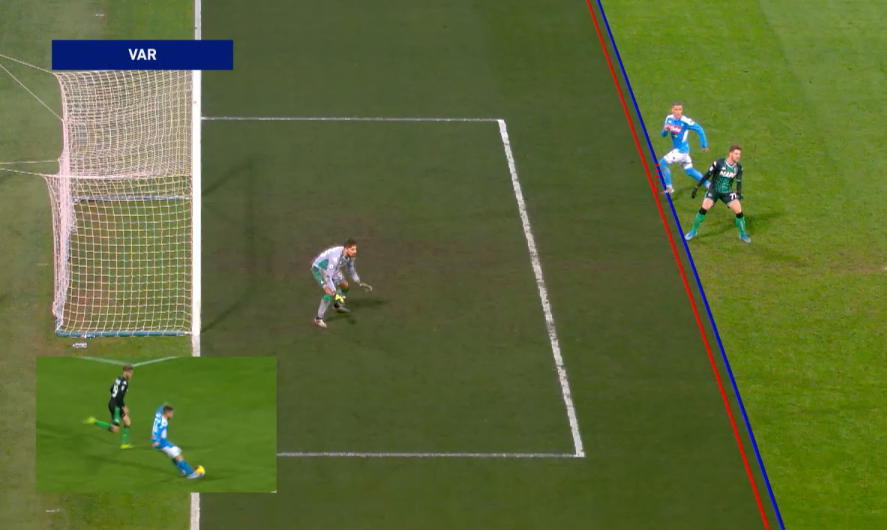
\includegraphics[scale=0.50]{var.png}
			
			\caption{Rappresentazione del fuorigioco} \label{fig:offside}
			Source: \url{https://sport.sky.it/calcio/2021/10/05/fifa-figc-var-fuorigioco}
		\end{center}
	\end{figure}
	
	È stata inserita perché, se una squadra viene colta molte volte in fuorigioco allora il suo gioco sarà interrotto con vantaggio della squadra avversaria che farà ripartire la sua azione a proprio favore.
	
\end{itemize}

\subsection{Dati relativi ai tiri}

In questo gruppo sono presenti le variabili collegata alla fase offensiva della squadra in esame.

\begin{itemize}
	
	\item \textsf{Sh}: indica il numero di tiri totali fatti dalla squadra specificata della variabile \textsf{Team}. Quindi vengono conteggiati il numero di tiri in porta più i tiri fuori dalla porta. 
	
	Una squadra che effettua tanti tiri ha più probabilità di segnare un gol. Occorre però capire quanto è precisa una squadra nel centrare la porta.
	\item \textsf{SoT}: Indica il numero di tiri in porta totali fatti dalla squadra specificata della variabile \textsf{Team}. 
	
	Una squadra con un alto valore di tiri in porta è più probabile che possa segnare un gol. \texttt{SoT} permette di capire quanto è precisa in combinazione con \texttt{Sh} la squadra di calcio nel centrare la porta.
	\item \textsf{G/Sh}: indica la proporzione tra gol e tiri fatti dalla squadra specificata della variabile \textsf{Team}. 
	
	Questo può permettere di capire quanto la produzione di tiri della squadra è efficace o meno. Con \texttt{Sh} e \texttt{SoT} si riesce a valutare quanto sia offensiva la squadra, cioè se essa gioca costantemente in attacco o utilizza la tattica "difesa e contropiede". Inoltre, permette di capire quanto la squadra sia precisa nell'effettuare i tiri in porta.
\end{itemize}

\subsection{Dati relati al possesso}

In questo gruppo sono contenute le variabili collegate al possesso della palla 

\begin{itemize}
	
	\item \textsf{Poss}: indica la quantità di tempo (in percentuale) di possesso palla durante una partita di calcio per la squadra specificata della variabile \textsf{Team}. Nel gioco del calcio, con il termine “possesso palla” si intende un’azione manovrata di due o più giocatori che riescono a passarsi la palla evitando i contrasti degli avversari. Durante la partita, ogni volta che una squadra ha il dominio della palla si dice che questa squadra è in fase di “possesso palla”, quindi in questa variabile viene indicato quanto questa fase è durata nell'intera partita.\\
	Il metodo più comune utilizzato per calcolare il possesso palla di una squadra si basa sull'utilizzo di tre cronometri, uno per ciascuna formazione più uno per i tempi morti. Quando un giocatore della squadra A tocca un pallone che prima era in possesso della squadra B, il cronometro della squadra A parte e quello della squadra B si ferma e così via. Il terzo cronometro registra il tempo in tutte le situazioni di palla inattiva, ad esempio, rimesse laterali, calci di punizione ecc... I tempi vengono poi trasformati in percentuali. Per una registrazione più sofisticata, si possono utilizzare ventidue cronometri, uno per ogni giocatore.
	
	La variabile è stata inserita perché, la supremazia nel possesso palla è solitamente desiderabile e utile, dati i seguenti vantaggi:
	\begin{itemize}
		\item spingere l’avversario a muoversi verso la palla per allontanarlo dalla difesa della propria porta per poi sorprenderlo negli spazi lasciati incustoditi.   
		\item modulare il ritmo della gara, ad esempio, se una squadra sta vincendo con un gol di scarto, "congela" il risultato mantenendo il possesso della palla in modo da non ricevere attacchi da parte della squadra avversaria.
	\end{itemize}
	Il possesso palla però non garantisce la vittoria. Produrre un possesso palla "sterile", cioè senza che questo porti alla produzione di azioni offensive, può esporre la squadra in possesso della palla a contropiedi nel caso in cui la palla venga persa e quindi all'alto rischio di subire gol perché sbilanciata e non ben posizionata. Vedremo di seguito quali variabili possono essere utili per capire se il possesso palla fatto dalla squadra è "sterile" oppure no.
	
	\item \textsf{ToDefPen}: indica il numero di tocchi fatti dai giocatori della squadra specificata della variabile \textsf{Team} nella propria area di rigore. 
	
	Questa variabile è stata inserita perché può essere utile per capire come venga gestito il possesso della palla. Se vi è un alto numero di tocchi, vuol dire che la squadra subisce molto la pressione della squadra avversaria, viceversa cerca di fare un gioco più offensivo. Questa variabile, in combinazione con le variabili \textsf{ToDef3rd}, \textsf{ToMid3rd}, \textsf{ToAtt3rd} e \textsf{ToAttPen} permette di capire se il possesso della palla fatto della squadra sia utile e porti benefici ai fini del risultato oppure sia sterile. Inoltre, si vuole capire in che misura come \textsf{ToDefPen} influenza il risultato della partita con un alto o un basso valore di numero di tocchi nella propria area di rigore, la cui area è indicata nella Figura \ref{fig:penalty}.
	
	\begin{figure}[!ht]
		\begin{center}
			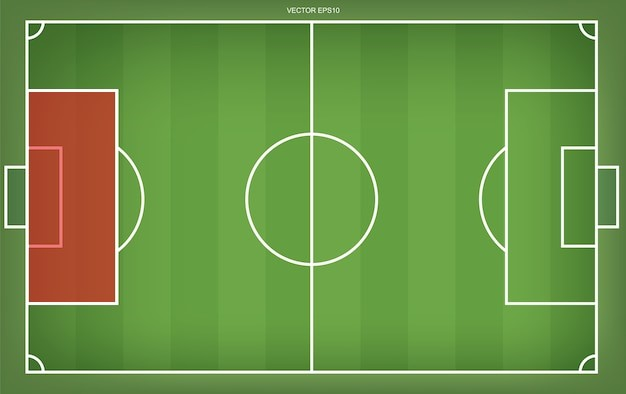
\includegraphics[scale=0.58]{rigore.jpg}
			\caption{In rosso l'area di rigore in un campo da calcio.}
			Source: \url{https://it.freepik.com/foto-vettori-gratuito/campo-da-calcio} 
			\label{fig:penalty}
		\end{center}
	\end{figure}
	
	
	\item \textsf{ToDef3rd}: indica il numero di tocchi fatti dai giocatori della squadra specificata della variabile \textsf{Team} nella propria mediana o trequarti difensiva. 
	
	Questa variabile è stata inserita perché può essere utile per capire come venga gestito il possesso della palla. Se vi è un alto numero di tocchi, vuol dire che la squadra cerca di mantenere il possesso palla creando poche azioni offensive, viceversa cerca di fare un gioco più offensivo. Questa variabile, in combinazione con \textsf{ToDefPen}, \textsf{ToMid3rd}, \textsf{ToAtt3rd} e \textsf{ToAttPen}, permette di capire se il possesso della palla fatto della squadra sia utile e porti benefici ai fini del risultato oppure sia sterile. Inoltre, si vuole capire in che misura \textsf{ToDef3rd} influenza il risultato della partita con un alto o un basso valore di numero di tocchi nella propria mediana la cui area, è indicata nella Figura \ref{fig:def}.
	
	\begin{figure}[!ht]
		\begin{center}
			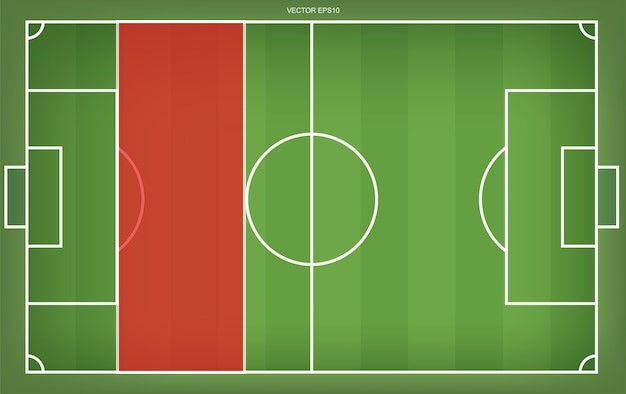
\includegraphics[scale=0.58]{mid.jpg}
			\caption{In rosso la mediana nel campo da calcio.} 
			Source: \url{https://it.freepik.com/foto-vettori-gratuito/campo-da-calcio} 
			\label{fig:def}
		\end{center}
	\end{figure}
	\item \textsf{ToMid3rd}: indica il numero di tocchi fatti dai giocatori della squadra specificata della variabile \textsf{Team} a centrocampo. 
	
	Questa variabile è stata inserita perché può essere utile per capire come venga gestito il possesso della palla. Se vi è un alto numero di tocchi, vuol dire che la squadra cerca di mantenere il possesso palla cercando di creare delle azioni offensive, viceversa cerca di fare un gioco più difensivo. Questa variabile, in combinazione con le variabili \textsf{ToDefPen}, \textsf{ToDef3rd}, \textsf{ToAtt3rd} e \textsf{ToAttPen}, permette di capire se il possesso della palla fatto dalla squadra sia utile e porti benefici ai fini del risultato oppure sia sterile. Inoltre, si vuole capire in che misura \textsf{ToMid3rd} influenza il risultato della partita con un alto o un basso valore di numero di tocchi a centrocampo la cui area, è indicata nella Figura \ref{fig:cen}.
	
	\begin{figure}[!ht]
		\begin{center}
			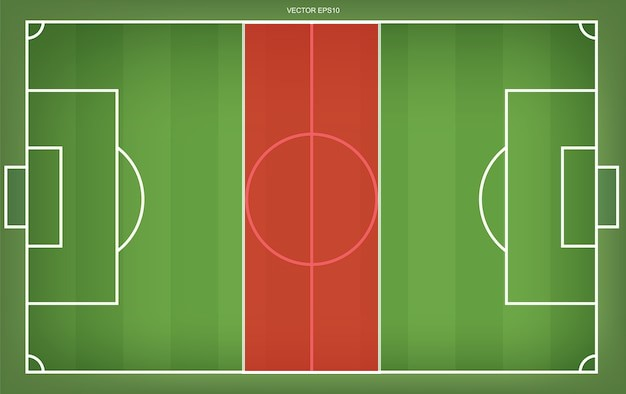
\includegraphics[scale=0.58]{cen.jpg}
			\caption{In rosso il centrocampo nel campo da calcio.}
			Source: \url{https://it.freepik.com/foto-vettori-gratuito/campo-da-calcio}  
			\label{fig:cen}
		\end{center}
	\end{figure}
	
	\item \textsf{ToAtt3rd}: indica il numero di tocchi fatti dai giocatori della squadra specificata della variabile \textsf{Team} a nella trequarti dell'avversario. 
	
	Questa variabile è stata inserita perché può essere utile per capire come venga gestito il possesso della palla. Se vi è un alto numero di tocchi, vuol dire che la squadra cerca di mantenere il possesso palla per effettuare una pressione sulla squadra avversaria affinché si possano creare degli spazi per delle azioni offensive, viceversa cerca di fare un gioco molto più difensivo. Questa variabile, in combinazione con le variabili \textsf{ToDefPen}, \textsf{ToDef3rd}, \textsf{ToMid3rd} e \textsf{ToAttPen}, permette di capire se il possesso della palla fatto della squadra sia utile e porti benefici ai fini del risultato oppure sia sterile. Inoltre, si vuole capire in che misura \textsf{ToAtt3rd} influenza il risultato della partita con un alto o un basso valore di numero di tocchi nella trequarti dell'avversario la cui area, è indicata nella Figura \ref{fig:treq}.
	
	\begin{figure}[!ht]
		\begin{center}
			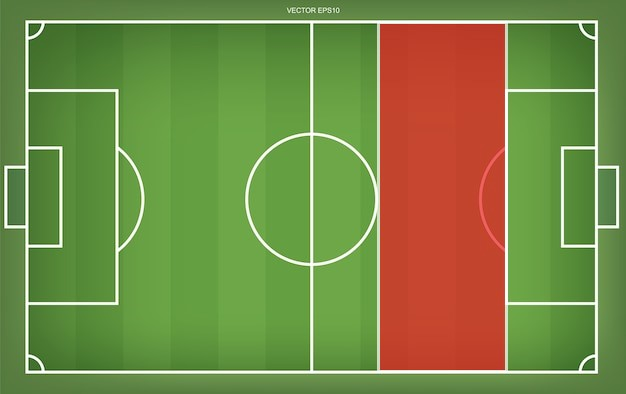
\includegraphics[scale=0.58]{treq.jpg}
			\caption{In rosso la trequarti dell'avversario nel campo da calcio.} 
			Source: \url{https://it.freepik.com/foto-vettori-gratuito/campo-da-calcio} 
			\label{fig:treq}
		\end{center}
	\end{figure}
	
	\item \textsf{ToAttPen}: indica il numero di tocchi fatti dai giocatori della squadra specificata della variabile \textsf{Team} a nell'area di rigore dell'avversario. 
	
	Questa variabile è stata inserita perché può essere utile per capire come venga gestito il possesso della palla. Se vi è un alto numero di tocchi, vuol dire che la squadra cerca di mantenere il possesso palla applicando un'alta pressione sulla squadra avversaria affinché si possano creare molte occasioni da gol in area, viceversa o la squadra subisce troppo la pressione dell'avversario oppure tende ad avere un gioco molto difensivo. Questa variabile, in combinazione con le variabili \textsf{ToDefPen}, \textsf{ToDef3rd}, \textsf{ToMid3rd} e \textsf{ToAtt3rd} permette di capire se il possesso della palla fatto della squadra sia utile e porti benefici ai fini del risultato oppure sia sterile. Inoltre, si vuole capire in che misura\textsf{ToAttPen} influenza il risultato della partita con un alto o un basso valore di numero di tocchi nell'area di rigore dell'avversario.
	
	\item \textsf{ToDist}: Indica la distanza totale, espressa in metri, in cui un giocatore della squadra specificata della variabile \textsf{Team} si è mosso con la palla in qualsiasi direzione, controllandola con i piedi.
	
	Questa variabile è stata inserita perché permette di comprendere se il possesso della palla sia stato statico, ovvero i giocatori si sono mossi poco senza avanzare, oppure no. Sarà di interesse analizzare se un alto valore di metri percorsi con palla al piede possa essere utile ad ottenere la vittoria.
	
\end{itemize}

\subsection{Dati relativi ai passaggi}
%SCRIVI SOLO "INDICA" SU TUTTE LE PROSSIME COME HO FATTO PRIMA: Tale variabile indica => indica

In questo gruppo vi sono raggruppate le variabili collegate ai passaggi della palla.

\begin{itemize}
	
	
	\item \textsf{PAtt}: Indica il numero di tutti i passaggi tentati dai giocatori della squadra specificata della variabile \textsf{Team}. 
	
	Utile a capire quanto la squadra sia incline a tentare i passaggi.
	
	\item\textsf{PCmp\%}: Indica la percentuale di passaggi riusciti ai giocatori della squadra specificata della variabile \textsf{Team}. 
	
	È stata inserita perché permette di capire quanti passaggi siano andati a buon fine tra tutti quelli tentati e quindi la precisione dei giocatori della squadra.
	\item \textsf{SPAtt}: Indica il numero di passaggi corti tentati dai giocatori della squadra specificata della variabile \textsf{Team}. Per passaggi corti si intendono tutti quelli effettuati all'interno di una lunghezza tra i tre e quattordici metri.
	
	È stata inserita per capire se un alto numero di passaggi corti possa essere determinanti ai fini dell'esito della partita. 
	
	\item \textsf{SPCmp\%}: Indica la percentuale di passaggi corti riusciti ai giocatori della squadra specificata della variabile \textsf{Team}. 
	
	È stata inserita perché permette di capire quanti passaggi andati a buon fine tra tutti quelli tentati e quindi la precisione dei giocatori della squadra.
	
	\item \textsf{MPAtt}: Indica il numero di passaggi medi tentati dai giocatori della squadra specificata della variabile \textsf{Team}. Per passaggi medi si intendono tutti quelli effettuati all'interno di una lunghezza tra i tredici e ventisette metri. Questi passaggi possono essere considerati come passaggi filtranti, cioè non diretti al proprio compagno di squadra ma verso un’area del campo dove il compagno di squadra deve andare a prendere la palla. Spesso questi passaggi vengono fatti per sorprendere la difesa avversaria ed evitare che la palla venga intercettata. Nella Figura \ref{fig:filt} viene mostrato l'esecuzione di un passaggio filtrante.
	
	\begin{figure}[ht]
		\begin{center}
			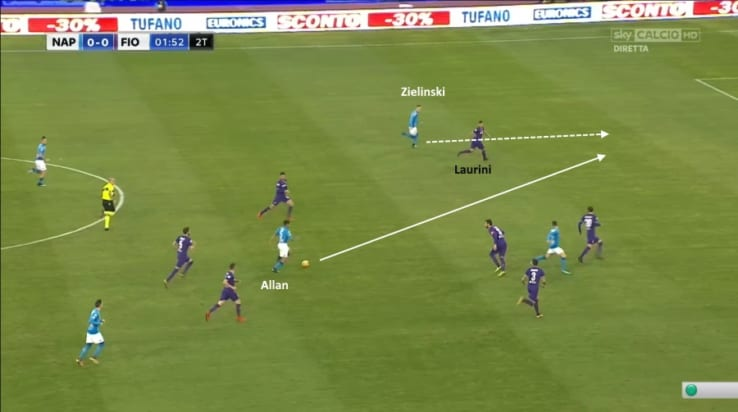
\includegraphics[scale=0.45]{filtrante2.jpg}
			\caption{Esecuzione di un passaggio filtrante} \label{fig:filt}
			Source: \url{https://www.ilmisterone.com/2019/01/16/passaggi-filtranti/}
		\end{center}
	\end{figure}
	
	È stata inserita per capire se un alto numero di passaggi medi possa essere determinante ai fini dell'esito della partita. 
	
	\item \textsf{MPCmp\%}: Indica la percentuale di passaggi medi riusciti ai giocatori della squadra specificata della variabile \textsf{Team}.\\ 
	
	È stata inserita perché permette di capire quanti passaggi siano andati a buon fine tra tutti quelli tentati e quindi la precisione dei giocatori della squadra.
	\item \textsf{LPAtt}: Indica il numero di passaggi lunghi tentati dai giocatori della squadra specificata della variabile \textsf{Team}. Per passaggi lunghi si intendono tutti quelli effettuati all'interno di una lunghezza superiore ai ventisette metri. Questi passaggi possono essere considerati come lanci lunghi per cambi di gioco o per lanciare le punte, cioè i giocatori che giocano come attaccanti, in profondità. Una rappresentazione di passaggio lungo è mostrata nella Figura \ref{fig:cambio}.
	\begin{figure}[ht]
		\begin{center}
			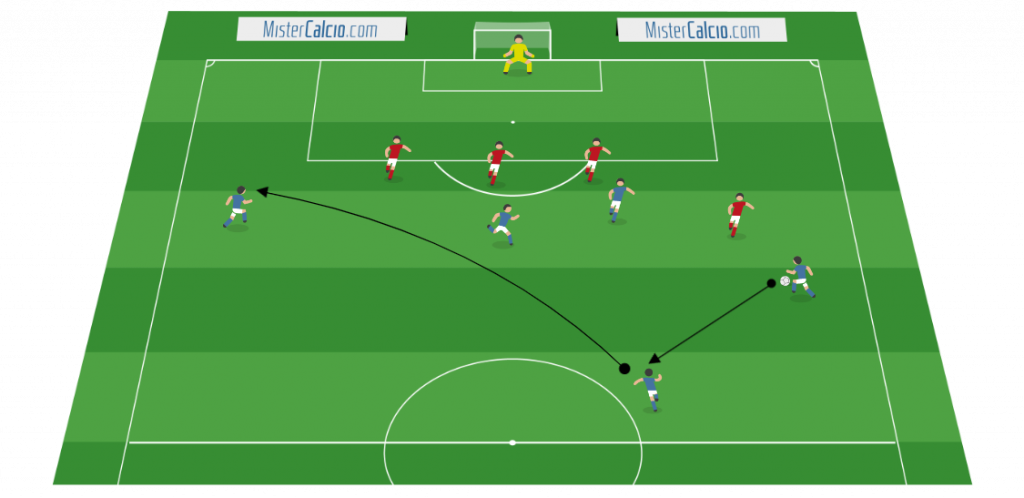
\includegraphics[scale=0.45]{cambio-di-gioco.png}
			\caption{Esecuzione di un cambio di gioco} \label{fig:cambio}
			Source: \url{https://www.mistercalcio.com/tattica/il-cambio-di-gioco/}
		\end{center}
	\end{figure}
	
	È stata inserita per capire se un alto numero di passaggi lunghi possa essere determinante ai fini dell'esito della partita.
	
	\item \textsf{LPCmp\%}: Indica la percentuale di passaggi lunghi riusciti ai giocatori della squadra specificata della variabile \textsf{Team}. 
	
	È stata inserita perché permette di capire quanti passaggi sono andati a buon fine tra tutti quelli tentati e quindi qual'è la precisione dei giocatori della squadra.
	
	\item \textsf{Crs}: Indica il numero di cross effettuati dalla squadra specificata della variabile \textsf{Team}. Un cross (in italiano traversone) è un tipo di passaggio medio o lungo, solitamente effettuato sulle fasce laterali dell'area avversaria o comunque vicino all'area avversaria, che permette al compagno di squadra posizionato vicino alla porta avversaria di colpire la palla al volo di testa oppure di piede per segnare un possibile gol. Quindi, se eseguito correttamente, il cross può diventare un assist, cioè l'ultimo passaggio per la realizzazione del gol. 
	
	\begin{figure}[!ht]
		\begin{center}
			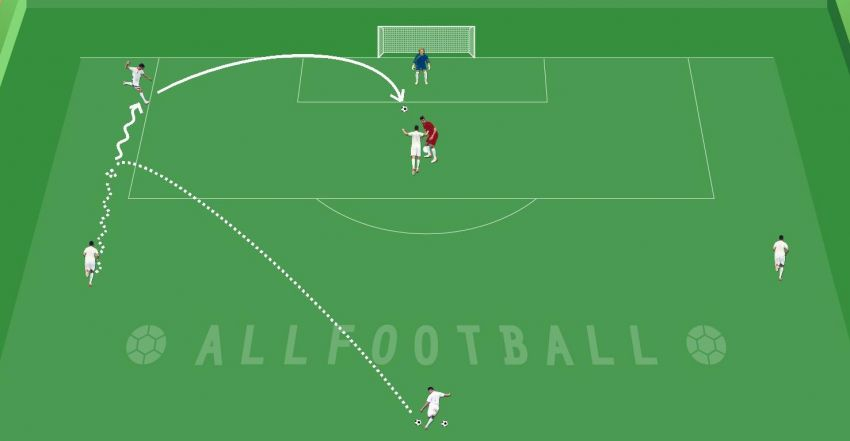
\includegraphics[scale=0.37]{cross.jpg}
			\caption{Rappresentazione di un cross} \label{fig:cross}
			Source: \url{http://www.allfootball.it/blog/calcio-vincere-allenando-i-dettagli/27-2-2017/calcio-la-marcatura-a-uomo-su-cross-laterale/}
		\end{center}
	\end{figure}
	
	Una rappresentazione di cross è mostrata nella Figura \ref{fig:cross}.
\end{itemize}

\subsection{Dati difensivi}

In questo gruppo sono contenute le variabili collegate alla fase difensiva.

\begin{itemize}
	
	\item \textsf{Saves}: Indica il numero di parate fatte del portiere della squadra specificata della variabile \textsf{Team}. 
	
	È stata inserita perché permette di valutare se la squadra subisce tanti tiri dagli avversari, così come la qualità del portiere nel salvare la squadra da un possibile gol subito.
	
	\item \textsf{Int}: Indica il numero di intercettazioni fatte dai giocatori della squadra specificata della variabile \textsf{Team}. Per intercettazione della palla si intende l'intercettazione di un passaggio della squadra avversaria entrando in possesso del pallone andando ad interrompere il passaggio avversario. 
	
	\item \textsf{TklWin}: Indica il numero di contrasti vinti dai giocatori della squadra specificata della variabile \textsf{Team}. Per contrasto si intende il tentativo da parte di un giocatore difendente di sottrarre il possesso della palla all'avversario. Quindi chi ha in possesso la palla viene attaccato da chi ne è privo. Se si riesce a prendere il pallone all'avversario allora si avrà vinto il contrasto. I contrasti vengono effettuati anche per allontanare l'avversario dalle zone pericolose. La Figura \ref{fig:tackle} mostra un contrasto di gioco.
	
	\begin{figure}[!ht]
		\begin{center}
			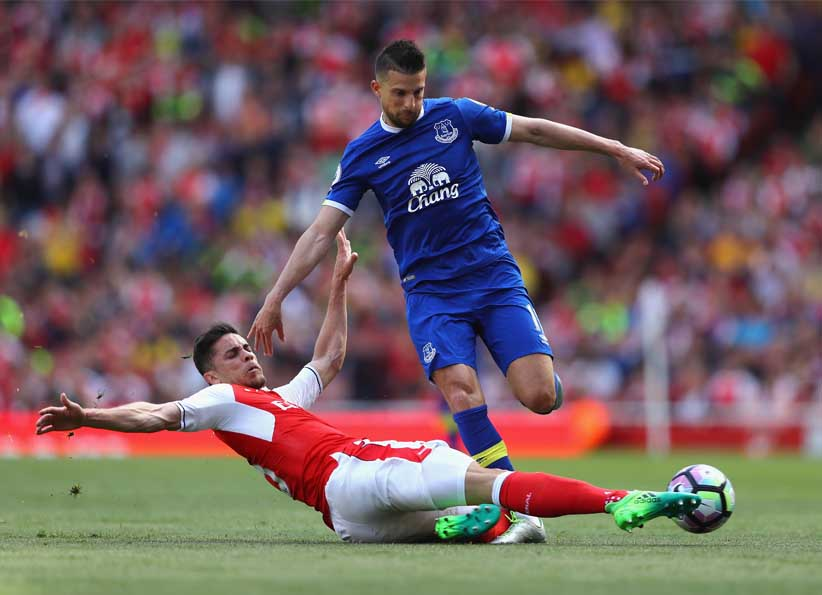
\includegraphics[scale=0.40]{tackle.jpg}
			\caption{Rappresentazione di un contrasto in scivolata}
			Source: \url{https://www.ilmisterone.com/2022/01/24/partita-solo-tackle/}
			\label{fig:tackle}
		\end{center}
	\end{figure}
	
	Visto che tale intervento senza palla modifica il gioco dell'avversario, si è deciso di inserire i contrasti vinti come variabile. 
	
	\item \textsf{Recov}: Indica il numero di palle vaganti recuperate dalla squadra specificata della variabile \textsf{Team}. Per palle vaganti si intendono quei palloni che, a seguito di un contrasto di gioco, non sono stati recuperati dalla squadra che ha effettuato il contrasto ma chi ha subito il contrasto, ne ha comunque perso il controllo. Quindi nessuno ha in possesso il pallone e la palla viene detta vagante.
	
	Dato che questa variabile sembra essere legata al possesso del pallone, potrebbe essere interessante per l'analisi.
	
	
\end{itemize}

Nella Tabella \ref{tab:summary} è riassunto l'insieme delle variabili presenti e le loro macro-aree di appartenenza.\\
\begin{table}[!htb]%
	
	\renewcommand{\arraystretch}{1.7}
	\centering
	\begin{tabular}{c c c c c}
		\hline	
		
		\textbf{Statistiche generali} & \textbf{Tiri} & \textbf{Possesso} & \textbf{Passaggi} & \textbf{Difensive} \\	
		\hline			
		AtHome & Sh & Poss & PAtt & Saves\\
		Res & SoT & ToDefPen & PCmp\% & Int\\
		GF & G/Sh & ToDef3rd & SPAtt & TklWin\\
		GA &  & ToMid3rd & SPCmp\% & Recov\\
		Team &  & ToAtt3rd & MPAtt&\\
		VS &  & ToAttPen & MPCmp\% &\\
		Fls &  & ToDist & LPAtt &\\
		Fld &  &  & LPCmp\% &\\
		Off &  &  & Crs \\
		\hline
		
		
	\end{tabular} \hbox{}
	
	\caption{La tabella riassuntiva variabili presenti nel \emph{dataset}.} \label{tab:summary}
\end{table}

Di seguito nella Tabella \ref{tab:summary2} è mostrato per ogni variabile il nome che ha all'interno del \emph{dataset}.


\begin{table}[!htb]%
	
	\renewcommand{\arraystretch}{1.7}
	\centering
	\begin{tabular}{c c }
		\hline	
		
		\textbf{Originale} & \textbf{Rinominate} \\	
		\hline			
		AtHome & AtHome \\
		Res & Res \\
		GF & GF\\
		GA & GF \\
		Team & Team \\
		VS & Vs\\
		Poss & Poss\\
		Sh & Sh\\
		SoT & SoT\\
		G/Sh & G.Sh \\
		Saves & Saves \\
		PAtt & PAtt \\
		PCmp\% & PCmp.\\
		SPAtt & SPAtt \\
		SPCmp\% & SPCmp.\\
		MPAtt & MPAtt \\
		MPCmp\% & MPCmp.\\
		LPAtt & LPAtt \\
		LPCmp\% & LPCmp. \\
		ToDefPen & ToDefPen \\
		ToDef3rd & ToDef3rd \\
		ToMid3rd & ToMid3rd \\
		ToAtt3rd & ToAtt3rd \\
		ToAttPen & ToAttPen \\
		ToDist & ToDist\\
		Fls & Fls \\
		Fld & Fld \\
		Off & Off \\
		Crs & Crs \\
		Int & Int \\
		TklWin & TklWin \\
		Recov & Recov \\
		\hline
		
	\end{tabular} \hbox{}
	
	\caption{Tabella corrispondenza nomi originali e nomi nel \emph{dataset}} \label{tab:summary2}
\end{table}
             % Dati
% !TEX encoding = UTF-8
% !TEX TS-program = pdflatex
% !TEX root = ../tesi.tex

%**************************************************************
\chapter{Analisi dei dati}
%\label{cap:flow engine}
%**************************************************************
\intro{Nel seguente capitolo verrà illustrata la fase di preprocessing e l'analisi grafica dei dati. }\\

%*************************************************************

\section{Preprocessing dei dati}
Dopo aver importato il dataset sul software R, il primo step da effettuare durante il prepocessing è individuare e risolvere possibili anomalie nei dati per poter poi effettuare analisi preliminari.\\
Il dataset è stato importato in modo tale che la prima riga contenga l'intestazione, mentre le restanti righe tutte le osservazioni. Il commando usato per importare il dataset è il seguente:\\

\begin{lstlisting}
> soccer<-read.xlsx("SerieA.xlsx", 1, header=TRUE)
\end{lstlisting}
\bigskip
Il dataset non ha valori mancanti dato. Questo è stato possibile grazie a una buona fonte di dati che ha messo a disposizione dati quasi sempre completi; in quei rari casi di mancanza di dati sono stati reperiti manualmente da altre fonti altrettanto attendibili.\\
Sono state inoltre tolte le variabili \texttt{Date} e \texttt{Round}.\\
Il passo successivo è stato controllare se le variabili venivano interpretate con il tipo corretto. Le variabili \texttt{Team} e \texttt{Vs} vengono interpretate erroneamente come tipo \texttt{character}. Queste variabili devono essere interpretate come fattore cioè un variabile non numerica, espressa in termini verbali ad esempio una categoria; quindi ogni squadra sarà un livello del fattore. Analogamente per \texttt{AtHome} vi è un interpretazione sbagliata; ciononostante si pensi che possa essere un tipo \texttt{logical} si è preferito convertire la variabile in un fattore con due livelli. Anche la variabile \texttt{Res} è stata trasformata in un fattore con i livelli; 1 = vittoria, 0 = pareggio, -1 = sconfitta.


\section{Analisi grafica dei dati}
In questa sezione attraverso il supporto di grafici, si analizzerà graficamente i dati disponibili e le loro relazione per avere una prima visione dei dati raccolti. Si cercherà di: individuare possibili outliers o anomalie, quali distribuzioni hanno i dati ma soprattutto valutare le relazione tra covariate e variabile di risposta e tra due covariate, con lo scopo di individuare quali covariate possono essere significative per la variabile risposta e quali interazioni tra covariate emergono dall'analisi grafica.\\

Come primo passo dell'analisi, viene valutata la distribuzione delle classi della variabile risposta \texttt{Res} all'interno delle osservazioni disponibili. Tale distribuzione è mostrata nella Figura \ref{fig:res}.

\begin{figure}[htbp]
	\begin{center}
		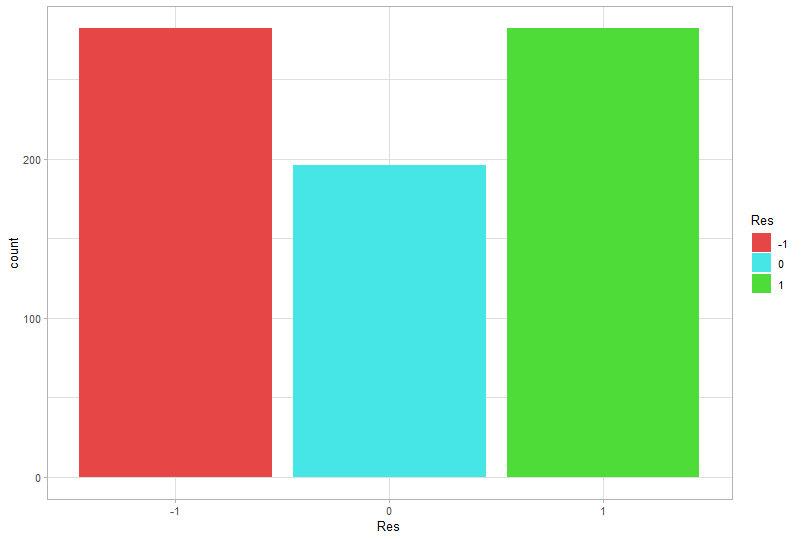
\includegraphics[scale=0.28]{barRes.png}
		\caption{Barplot della distribuzione della variabile di risposta \texttt{Res}} \label{fig:res}
	\end{center}
\end{figure}

Come si può notare le classi sembrano ben distribuite dato che abbiamo 196 pareggi e 282 vittorie e altrettante sconfitte. Si ha quindi un campione abbastanza ampio e distribuito e corretto per le nostre analisi.\\

Aumentando il livello di dettaglio è di interessante analizzare come queste classificazione sono distribuite tra le varie squadre.

\begin{figure}[htbp]
	\begin{center}
		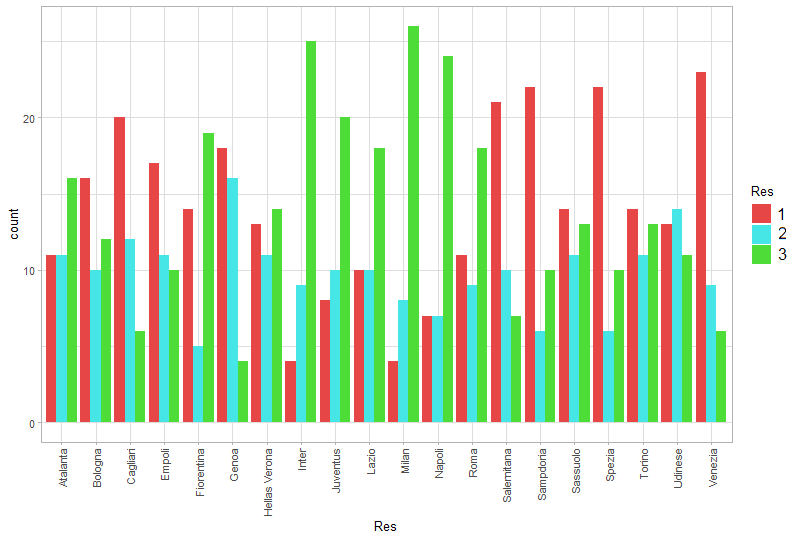
\includegraphics[height=8cm,width=15cm]{ResTeam.png}
		\caption{Barplot della distribuzione della variabile di risposta per squadra\texttt{Res}} \label{fig:team}
	\end{center}
\end{figure}

Nella Figura \ref{fig:team} si può notare come la distribuzione di vittorie, pareggi e sconfitte non è omogenea tra le squadre. Ovviamente è un risultato che ci si aspettava ma che sottolinea prima di tutto la correttezza dei dati ma soprattutto che vi è qualche elemento nascosto che ha determinato tale distribuzione.\\

\subsection{Analisi relazione tra variabile risposta e covariate}
Come secondo step si analizzerà le relazione tra variabile di risposta con alcune covariate.\\

La prima relazione che si analizza è quella con la variabile categorica \texttt{AtHome}. Nella Figura \ref{fig:AtHome} si può vedere che c'è una leggera variazione dei risultati tra la squadra che gioca in casa oppure no. Infatti c'è una leggera tendenza a favorire la vittoria per la squadra che gioca in casa piuttosto che la vittoria per la squadra fuori casa. Naturalmente non deve esserci alcuna variazione per quanto riguarda il pareggio dato che entrambe le squadre lo ottengono. Risulta perciò significativa la variabile \texttt{AtHome}.\\

\begin{figure}[htbp]
	\begin{center}
		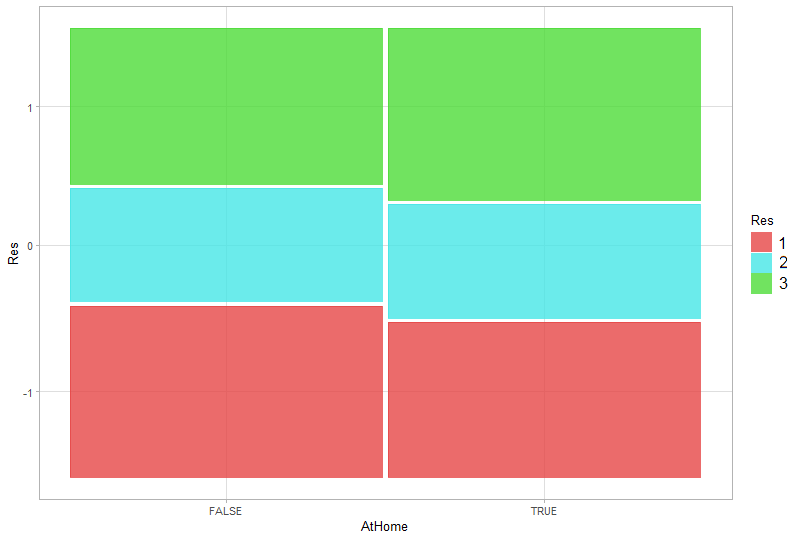
\includegraphics[scale=0.40]{AtHomeRes.png}
		\caption{Mosaicplot che mostra la distribuzione degli esiti rispetto alle partite giocate in casa e fuori casa} \label{fig:AtHome}
	\end{center}
\end{figure}

Analizzando invece la relazione tra variabile di risposta e \texttt{Poss}, dalla Figura \ref{fig:Poss} si nota che tale variabile sembra essere significativa per l'esito. Infatti vi è un relazione positiva dove valori più alti di possesso palla sono registrati nel box della vittoria e ciò può portare a una maggiore probabilità di vittoria. Vi è una buona distribuzione dei dati, infatti le code sono simmetriche mentre vi è una variabilità quasi identica; si segnala solo che la mediana della sconfitta è più vicina al 3$^{\circ}$ quantile mentre quella della vittoria è più vicina al 1$^{\circ}$ quantile. Inoltre non vi sono presenti outliers.

\begin{figure}[htbp]
	\begin{center}
		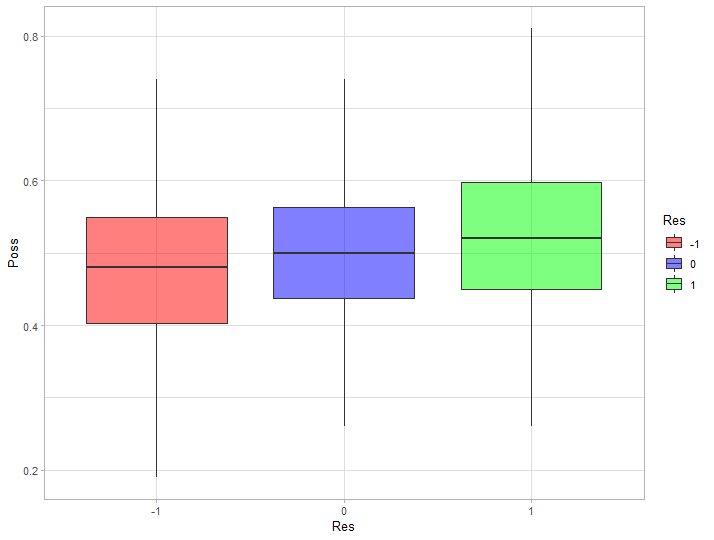
\includegraphics[scale=0.40]{Poss.png}
		\caption{Boxplot della variabile risposta e della variabile numerica \texttt{Poss} } \label{fig:Poss}
	\end{center}
\end{figure}

La Figura \ref{fig:sot} mostra come si comporta la relazione con \texttt{SoT}. Come ci si aspetta si hanno valori più alti nella vittoria e valori molto più bassi nella sconfitta, si ha una buona distribuzione dei valori nella vittoria dato che le code sono simmetriche, per le altre due classi non c'è simmetria dato che ci sono valori più bassi rispetto a valori più alti. Vi sono inoltre alcuni outliners che si discostano dalla distribuzione di tutte e tre le classi dovuti al fatto che ci sono state squadre che hanno tirato molto in porta. Le mediane dei box pareggio e vittoria non sono equidistanti dai quantili ma più vicine al 1$^{\circ}$ quantile. Il box della sconfitta ha una bassa varianza. In conclusione avere un valore alto di tiri in porta sembra essere significativo ai fini della vittoria. Si segnala inoltre che si ottengono i stessi risultati anche con \texttt{Sh} solo con valori meno alti per la vittoria rispetto a \texttt{SoT}.\\

\begin{figure}[htbp]
	\begin{center}
		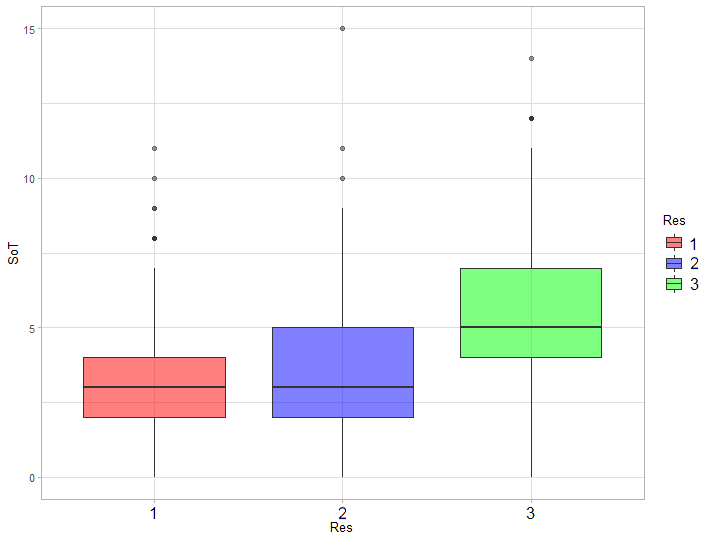
\includegraphics[scale=0.40]{SoT.png}
		\caption{Boxplot della variabile risposta e della variabile numerica \texttt{SoT} } \label{fig:sot}
	\end{center}
\end{figure}

La Figura \ref{fig:g} mostra come si comporta la relazione con \texttt{G/Sh}. Si nota che vi sono valori molto bassi ma leggermente più alti per la vittoria. La distribuzione non è buona perché le code sono asimmetriche infatti tutti i valori sono concentrati in basso e pochi verso la coda in alto, per di più c'è una bassa varianza tra i valori. Vi è la presenza di outliners dovuti a partite dove le squadre sono riuscite a ottenere il massimo da ogni tiro. I risultati mostrati nonostante la pessima distribuzione, sono comunque coerenti dato che non ci si aspetta dal rapporto tiri gol un numero alto ma comunque una tendenza che favorisca la vittoria.\\

\begin{figure}[htbp]
	\begin{center}
		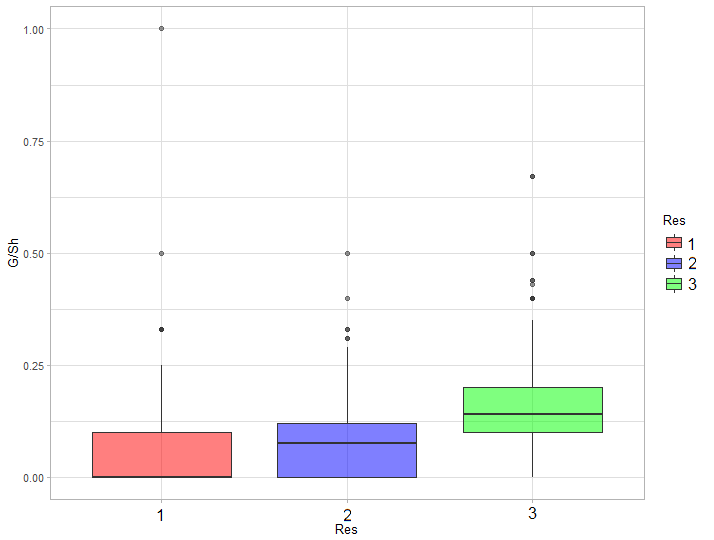
\includegraphics[scale=0.40]{g.png}
		\caption{Boxplot della variabile risposta e della variabile numerica \texttt{G/Sh} } \label{fig:g}
	\end{center}
\end{figure}

La Figura \ref{fig:saves} mostra come si comporta la relazione con \texttt{Saves}. Come si può notare sembra che tale variabile sia poco significativa ai fini del risultato. Infatti c'è poca variazione tra una classe e l'altra dato che avere un alto numero di parate non è determinante a fini del risultato.\\

\begin{figure}[htbp]
	\begin{center}
		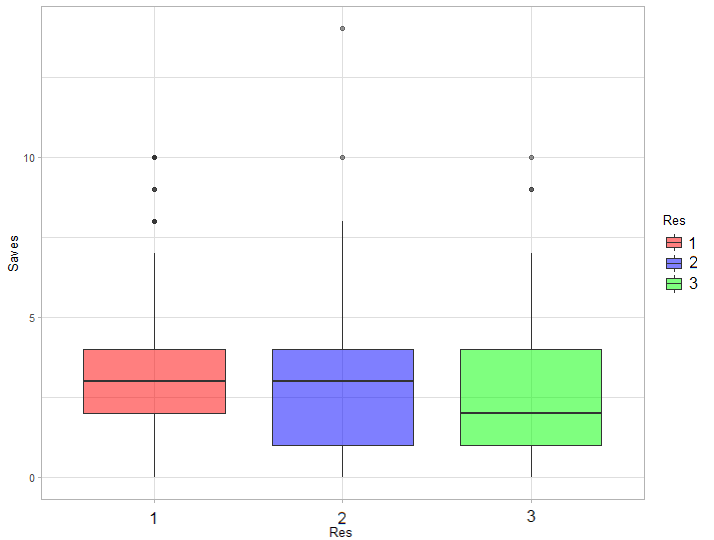
\includegraphics[scale=0.40]{saves.png}
		\caption{Boxplot della variabile risposta e della variabile numerica \texttt{Saves} } \label{fig:saves}
	\end{center}
\end{figure}

La Figura \ref{fig:pass} mostra come si comporta la relazione con \texttt{PAtt} e con \texttt{PCmp\%}. Per entrambi sembra significativo l'alto numero di passaggi tentati ma soprattutto quelli completati ai fini della vittoria. Nel primo boxplot la coda più in alto è più lunga rispetto alla coda in basso, quindi abbiamo valori più concentrati verso il basso che verso l'alto. Sempre nel primo boxplot il box della vittoria ha una maggiore variabilità rispetto ai altri due è varia di più avendo valori più alti; sia la mediana del box vittoria e sia quello del pareggio sono più vicine al 1${^\circ}$ quantile, viceversa quella della sconfitta. I dati nel primo boxplot sembrano essere coerenti con l'esito della partita dato che maggior numero di passaggi si prova ad effettuare maggiori sono le possibilità di vittoria, occorre pero sapere quanto è precisa la squadra.\\
Nel secondo boxplot si notano valori alti e molti outliners con valori bassi dovuti al fatto che ci sono state partite dove alcune squadre sono state poco precise nei passaggi. A differenza del primo boxplot il secondo boxplot ha molti valori alti, infatti la coda in alto e molto meno lunga rispetto alla coda in basso e le variabilità dei box sembrano essere uguali tra di loro; anche qui le code non sono simmetriche e quindi non c'è una buona distribuzione dei dati. Sorprendentemente sembra che avere un buona precisione pero non da la sicurezza di una vittoria, inoltre l'andamento prima scende da sconfitta a pareggio e poi sale da pareggio a vittoria.\\
Per quanto riguarda le variabili delle altre tipologie di passaggi si discostano di poco dai boxplot in Figura \ref{fig:pass}

\begin{figure}[htbp]
	\begin{center}
		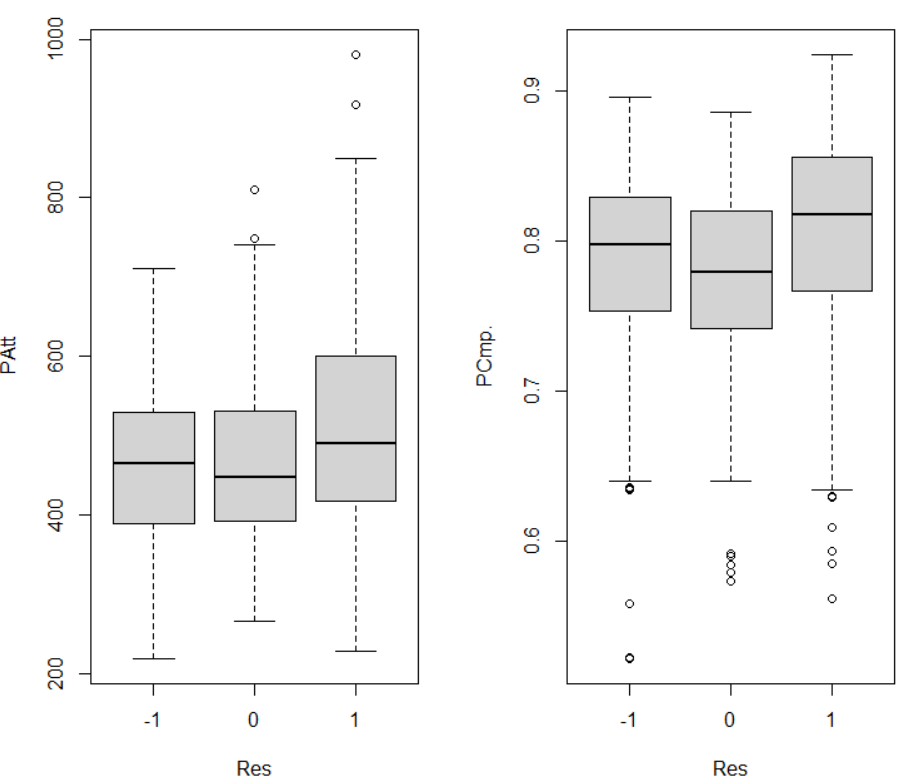
\includegraphics[scale=0.50]{pass.png}
		\caption{Boxplot della variabile risposta e della variabile numerica \texttt{PAtt} e \texttt{PCmp\%}  } \label{fig:pass}
	\end{center}
\end{figure}
\bigskip
La Figura \ref{fig:defp} mostra come si comporta la relazione con \texttt{ToDefPen}. Come si può notare questa non è per nulla significativa per la variabile risposta, infatti non c'è una minima variazione e i box hanno tutti la stessa varianza. Tale esito può essere giustificato dal fatto che le squadre cercano di rimane fuori il più possibile dalla propria area di rigore per non portare troppo vicino alla porta l'avversario. Da ciò quindi tale variabile non sarà inserita nel modello.\\

\begin{figure}[htbp]
	\begin{center}
		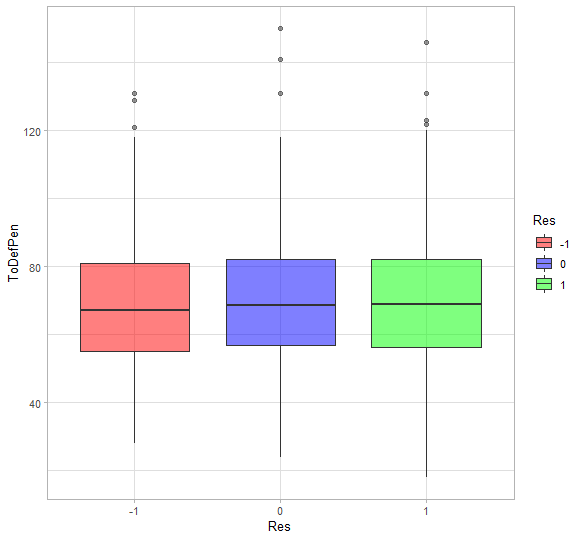
\includegraphics[scale=0.40]{def.png}
		\caption{Boxplot della variabile risposta e della variabile numerica \texttt{ToDefPen} } \label{fig:defp}
	\end{center}
\end{figure}

La Figura \ref{fig:defp} mostra come si comporta la relazione con \texttt{ToAttPen}. Contrariamente quanto visto con la Figura \ref{fig:defp} qui si nota una certa variazione da una un box e l'altro, infatti vi è una tendenza positiva che porta ad aver valori più alti in caso di vittoria. Si ha una maggior varianza per quanto riguarda la vittoria rispetto ai altri due esiti e la distribuzione di tutti e tre è abbastanza bilanciata se non che la coda più bassa è leggermente meno lunga rispetto all'altra coda; la mediana invece è equilibrata. Si nota inoltre che vi sono alcuni outliners segno che alcune squadre in qualche partite, si sono particolarmente rese note nel produrre un quantitativo di tocchi maggiore rispetto alla distribuzione, ciò pero non sembra influenzare l'esito.\\

Per quanto riguarda \texttt{ToDef3rd}, \texttt{ToMid3rd} e \texttt{ToAtt3rd}, esse si comportano come \texttt{ToAttPen}. Perciò è stato omesso il loro grafico.\\

\begin{figure}[htbp]
	\begin{center}
		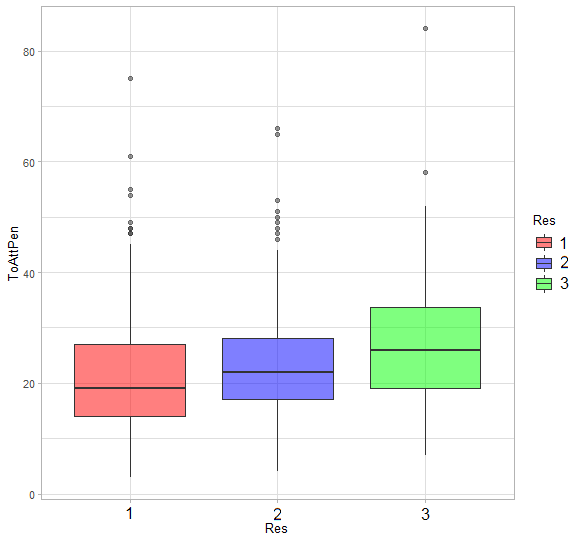
\includegraphics[scale=0.40]{att.png}
		\caption{Boxplot della variabile risposta e della variabile numerica \texttt{ToAttPen} } \label{fig:att}
	\end{center}
\end{figure}

Nella Figura \ref{fig:falli} vengono mostrati gli andamenti delle variabile dei falli, \texttt{Fls} e \texttt{Fld}. Nel boxplot a sinistra si può notare che i valori più alti sono nel box del pareggio mentre sono presenti valori più bassi nel box vittoria. Ciò fa pensare che subire molti falli può impedire la vittoria alla squadra che li subisce. Per quanto riguarda la distribuzione sembra essere buona; c'è minor varianza per quanto riguarda la sconfitta. \\

\begin{figure}[htbp]
	\begin{center}
		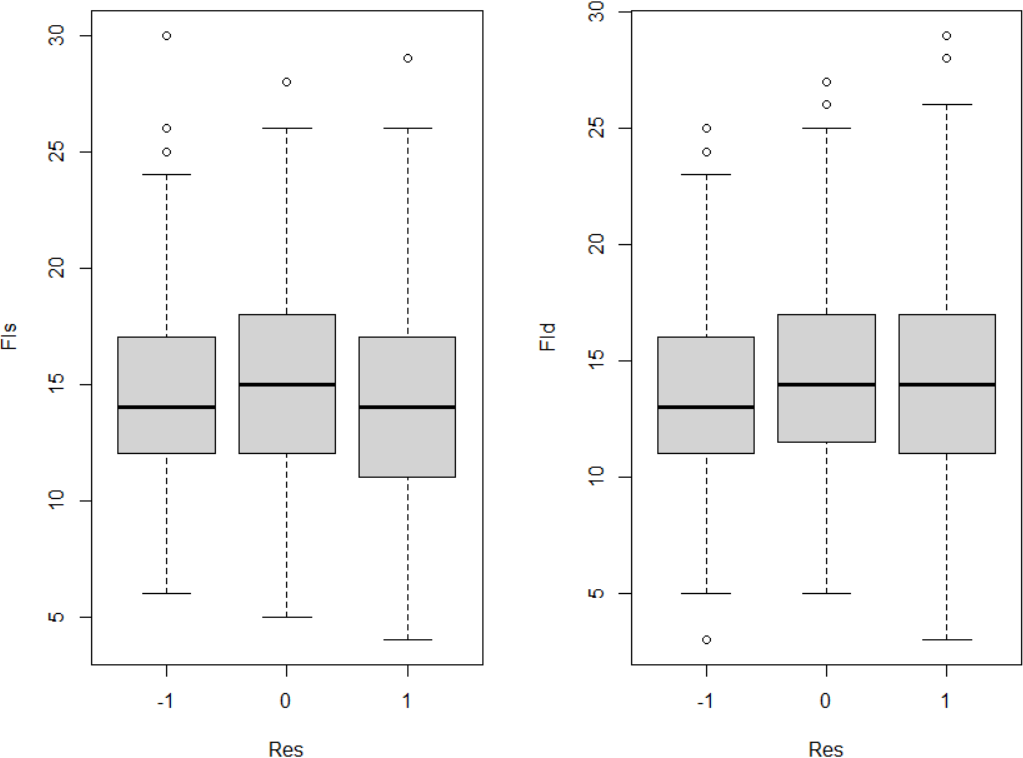
\includegraphics[scale=0.40]{falli.png}
		\caption{A sinistra il boxplot della variabile risposta e della variabile numerica \texttt{Fls} e a destra il boxplot della variabile risposta e della variabile numerica \texttt{Fld} } \label{fig:falli}
	\end{center}
\end{figure}

Nel secondo boxplot si può notare che i valori più alti sono presenti sia sul pareggio e sia sulla vittoria e sempre qui si ha una maggior distribuzione rispetto alla sconfitta. Sembra perciò che dal grafico si può intuire che se la squadra non commette dei falli allora sarà più soggetta a perdere.\\

La Figura \ref{fig:int} mostra come si comporta la relazione con \texttt{Int}. Sorprendentemente valori più alti sono registrati nella sconfitta, anche se la mediana risulta essere più vicina al 1 $^{\circ}$ quantile sottolineando che vi è un maggior numero di valori bassi piuttosto che alti. La mediana dei restanti esiti invece e ben equilibrata ma il pareggio risulta avere meno variabilità. Sembra perciò che effettuare troppi intercettazioni dei passaggi avversari contrariamente da quanto si pensi sembra essere controproducente per la vittoria. Si segnala inoltre la presenza di alcuni outliners con valori alti di intercettazioni, che si discostano dalle distribuzioni.\\

\begin{figure}[htbp]
	\begin{center}
		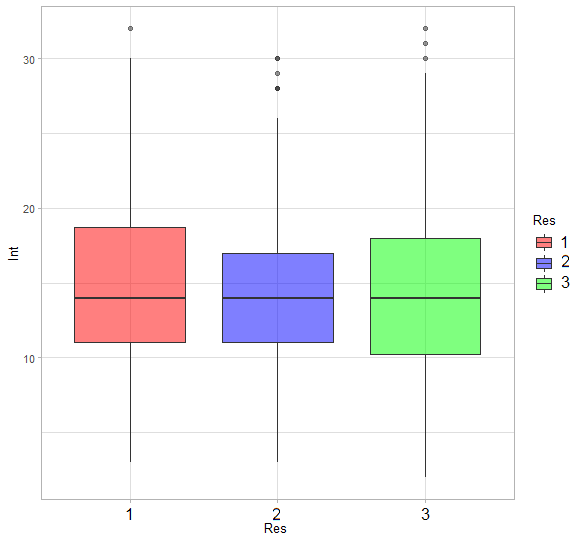
\includegraphics[scale=0.40]{int.png}
		\caption{Boxplot della variabile risposta e della variabile numerica \texttt{Int}} \label{fig:int}
	\end{center}
\end{figure}

La Figura \ref{fig:tkl} mostra come si comporta la relazione con \texttt{TklWin}. Come si può notare, vincere più contrasti possibili evita di subire una sconfitta. Infatti vi sono valori più alti in pareggio e vittoria oltre a una maggiore varianza rispetto alla sconfitta. Nello specifico pero si nota che, nella distribuzione dei valori vi sono maggior valori alti nella vittoria rispetto al pareggio, graficamente lo si vede dalla mediana che nel pareggio è più vicina al 1$^{\circ}$ quindi a valori più bassi e lo si nota anche dalla coda più bassa che è meno lunga rispetto a quella in alto; invece la mediana della vittoria risulta più vicina al 3$^{\circ}$ oltre ad avere la coda in alto più corta rispetto a quella in basso. Vi è inoltre qualche outliners con valori più alti di contrasti vinti ma sembrano non influenzare la classificazione.\\

\begin{figure}[htbp]
	\begin{center}
		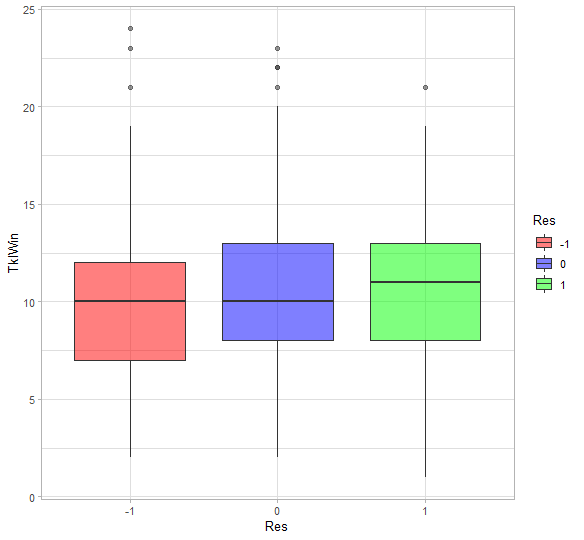
\includegraphics[scale=0.40]{tklwin.png}
		\caption{Boxplot della variabile risposta e della variabile numerica \texttt{TklWin}} \label{fig:tkl}
	\end{center}
\end{figure}

\begin{figure}[htbp]
	\begin{center}
		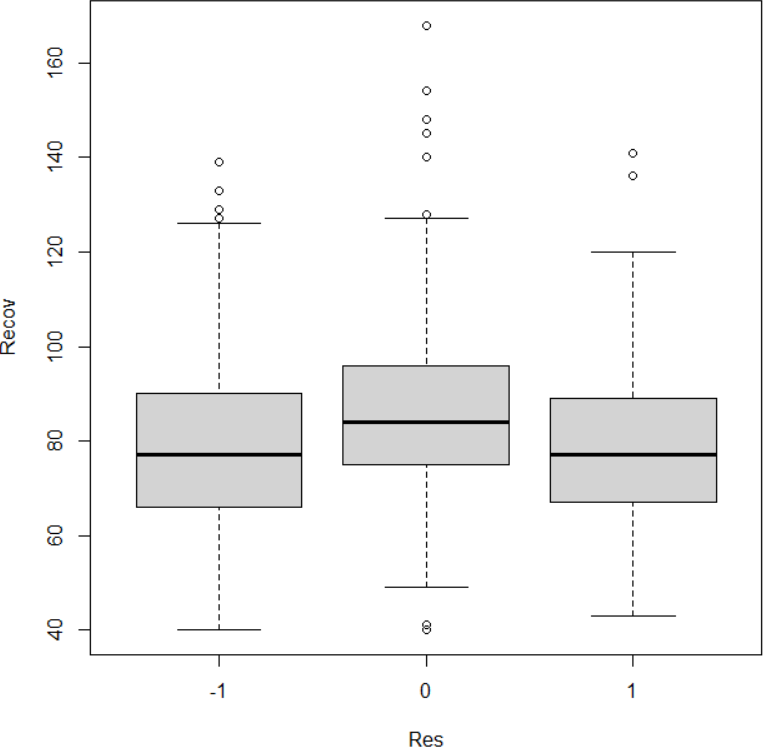
\includegraphics[scale=0.40]{recov.png}
		\caption{Boxplot della variabile risposta e della variabile numerica \texttt{Recov}} \label{fig:recov}
	\end{center}
\end{figure} 

Infine la Figura \ref{fig:recov} mostra come si comporta la relazione con \texttt{Recov}. Per entrambe le classi la distribuzione sembra più sbilanciata verso valori bassi quindi ad una loro maggior presenza, infatti entrambe le code più in basso sono più corte rispetto a quelle più in alto che sono più lunghe. Per quanto riguarda la mediana sembra per entrambe le classi equidistante dai quantili. Si nota che il pareggio presenta minor varianza rispetto alle altre due classi ma valori più alti soprattutto nei confronti della vittoria oltre ad averne anche di più rispetto alle altre classi. Sembra perciò che un eccessivo numero di recuperi non porti alla vittoria. Si nota inoltre che vi sono numerosi outliners sopratutto per il pareggio.

\subsection{Analisi relazioni tra covariate} 
Per concludere l'attività di prepossening, non resta che analizzare le relazioni tra covariate in modo da individuare possibili interazioni tra di loro che possono influenzare la variabile risposta. Chiaramente dato che vi sono più di 30 variabili e dunque, un grandissimo numero di combinazioni, non si sono esaminate tutte le relazioni ma sono state selezionate solo alcune per l'analisi basandosi su teorie calcistiche esaminate durante la fase di studio del problema.\\
Di seguito si riporteranno quelle che sono state individuate come significative.\\

Sono state individuate le seguenti tre interazioni con la variabile \texttt{Sh}:
\begin{itemize}
	\item Interazione tra \texttt{Sh} e \texttt{SoT}. Chiaramente vi si può dedurre facilmente che vi possa essere una buona correlazione tra queste due variabili perché teoricamente più tiri vengono effettuati maggiori saranno i tiri in porta. \\
	Tale relazione viene anche mostrata graficamente, infatti nella Figura \ref{fig:ShSoT} si può notare che vi è un'andamento positivo tra le due variabili, al cresce di una vi è un aumento quasi lineare dell'altra.
	Come si può notare dai colori inseriti nel grafico per indicare le tre classi della variabile risposta, l'effetto combinato delle due variabili è utile a spiegare la variabile risposta dato che, valori più bassi sono quasi sempre classificati come sconfitta, un po' più alti come pareggio, mentre quelli alti sono quasi sempre classificati come vittoria.
	Molte volte i valori vengo ripetuti per molte osservazione, quindi i valori nel grafico sono disposti in colonne e non sparsi.
	\begin{figure}[htbp]
		\begin{center}
			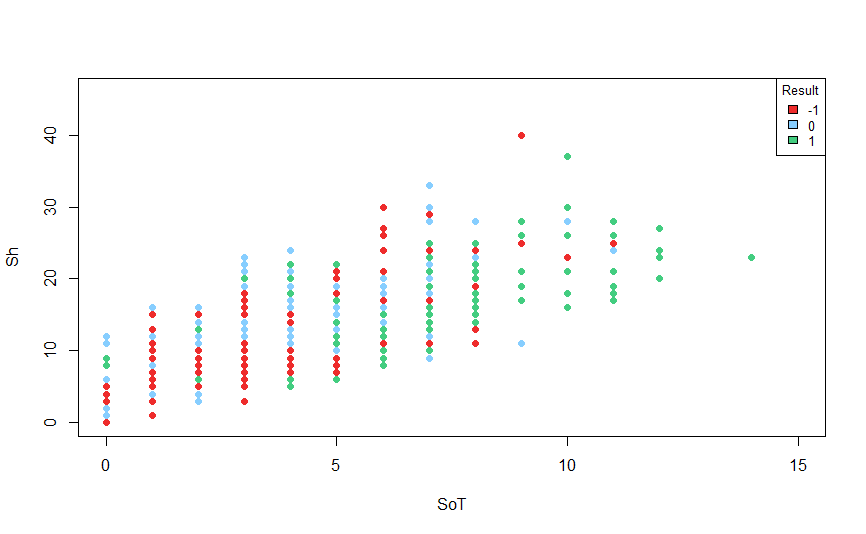
\includegraphics[scale=0.60]{sh-sot.png}
			\caption{Scatter plot tra \texttt{Sh} e \texttt{SoT}} \label{fig:ShSoT}
		\end{center}
	\end{figure} 
	\item Interazione tra \texttt{Sh} e \texttt{ToAtt3rd}. È ragionevole ipotizzare che il numero di tocchi fatti nella trequarti avversaria possano creare azioni che portano ad effettuare un tiro verso la porta avversaria; è quindi possibile che tra le due variabili vi possa esserci una relazione. L'ipotesi è avvalorata dalla Figura \ref{fig:shtreq} dove è presente una tendenza positiva quasi lineare tra le due variabili oltre a tre distribuzioni differenti dei dati in base alla loro classificazione.
	\begin{figure}[htbp]
		\begin{center}
			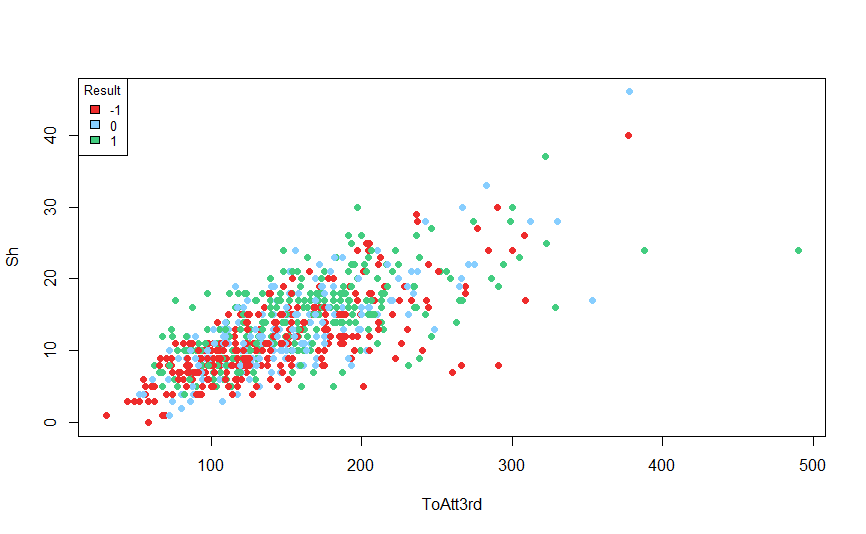
\includegraphics[scale=0.60]{sh-toatt3rd.png}
			\caption{Scatter plot tra \texttt{Sh} e \texttt{ToAtt3rd}} \label{fig:shtreq}
		\end{center}
	\end{figure}
	\item Interazione tra \texttt{Sh} e \texttt{ToAttPen}. Per la stessa ipotesi esposta nel punto precedente si è ipotizzato a tale interazione. La Figura \ref{fig:shpen} mostra che tale interazione è giustificata da una tendenza positiva nel cresce delle due variabili oltre a tre distribuzioni differenti dei dati in base alla loro classificazione. Si nota graficamente una maggior linearità rispetto alla Figura \ref{fig:shtreq}; ciò è coerente con il fatto che i tocchi vengono effettuati all'interno dell'area di rigore avversaria e quindi ad una distanza ravvicinata dalla porta, ne consegue una maggior possibilità di effettuare tiri in porta.
	\begin{figure}[htbp]
		\begin{center}
			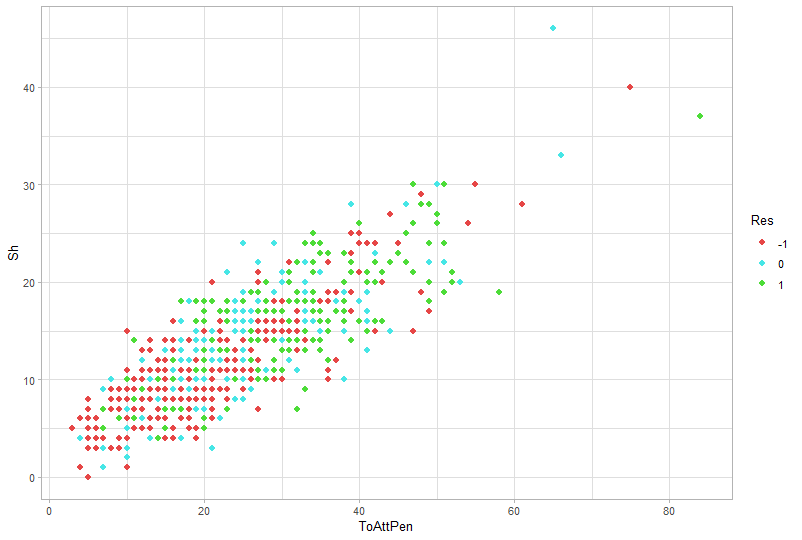
\includegraphics[scale=0.60]{sh-toattpen.png}
			\caption{Scatter plot tra \texttt{Sh} e \texttt{ToAttPen}}  \label{fig:shpen}
		\end{center}
	\end{figure}
\end{itemize}

Sono state individuate le seguenti tre interazioni con la variabile \texttt{Poss}:
\begin{itemize}
	\item Interazione tra \texttt{Poss} e \texttt{PAtt}. È ragionevole ipotizzare che il possesso della palla possa incidere su quanto una squadra tenti di effettuare passaggi, cioè da un alto possesso della palla ci si aspetta un alto numero di passaggi tentati, viceversa con un valore basso di possesso. L'ipotesi è confermata dalla Figura \ref{fig:posspatt} che mostra una relazione positiva è fortemente lineare tra le due ipotesi, oltre ad essere utili per spiegare l'andamento delle tre classi della variabile risposta.
	\begin{figure}[htbp]
		\begin{center}
			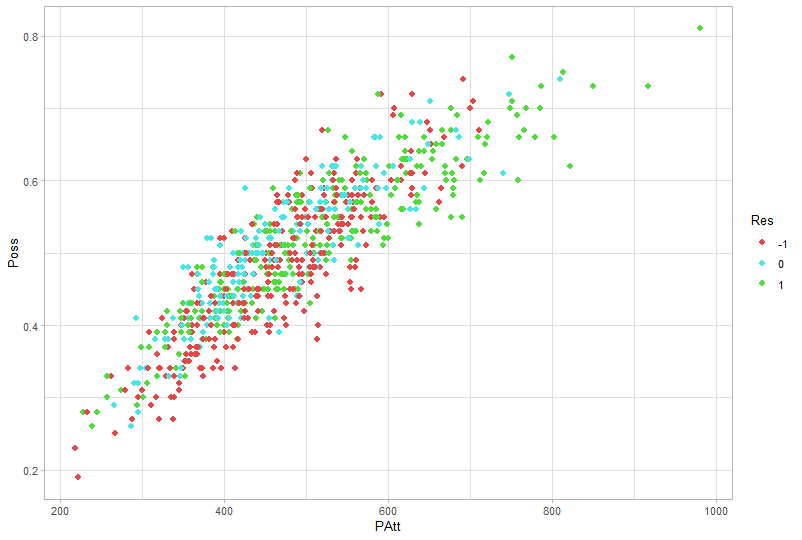
\includegraphics[scale=0.60]{poss-patt.png}
			\caption{Scatter plot tra \texttt{Poss} e \texttt{PAtt}}  \label{fig:posspatt}
		\end{center}
	\end{figure}
	\item Interazione tra \texttt{Poss} e \texttt{TotDist}. Appare naturale ipotizzare che il possesso della palla la distanza percorsa con il pallone siano in relazione tra loro. È altrettanto naturale aspettarci da un alto possesso della palla un alto numero di metri percorsi con la palla in possesso, viceversa con un valore basso di possesso. L'ipotesi è confermata dalla Figura \ref{fig:posstotdist} che mostra una relazione positiva abbastanza lineare tra le due ipotesi. Si segnala pero che dal grafico sembra che non vi sia una chiara divisione delle osservazioni in tre gruppi, tale aspetto sarà tenuto in considerazione nella modellazione.
	\begin{figure}[htbp]
		\begin{center}
			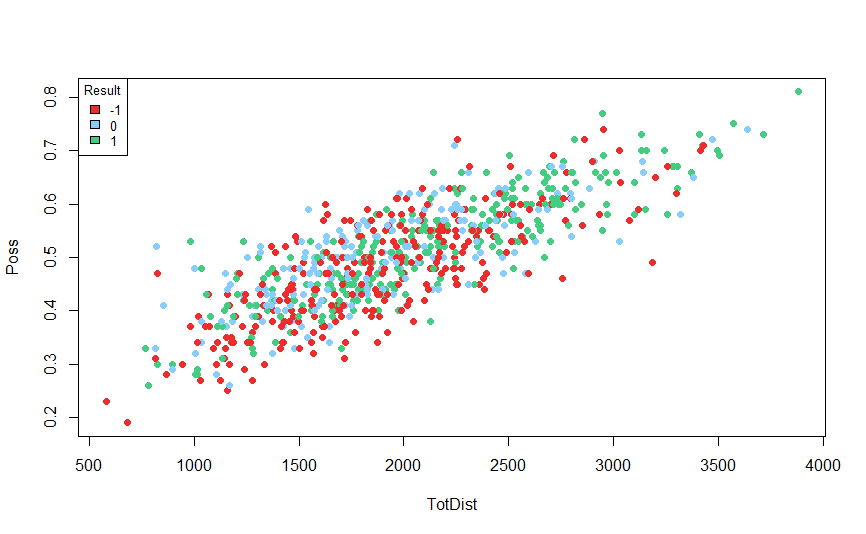
\includegraphics[scale=0.60]{poss-totdist.png}
			\caption{Scatter plot tra \texttt{Poss} e \texttt{TotDist}}  \label{fig:posstotdist}
		\end{center}
	\end{figure}
\end{itemize}
\pagebreak
Sono state individuate le seguenti tre interazioni con la variabile \texttt{TotDist}:
\begin{itemize}
	\item Interazione tra \texttt{TotDist} e \texttt{PAtt}. Dato che per poter tentare di effettuare passaggi è possibile farlo solo se ci si muove con la palla, allora è possibile ipotizzare che vi sia una relazione tra queste variabili. Dalla Figura \ref{fig:totdistpatt} si può notare che tra le due variabili vi è una forte relazione lineare e con una correlazione positiva.
	\begin{figure}[htbp]
		\begin{center}
			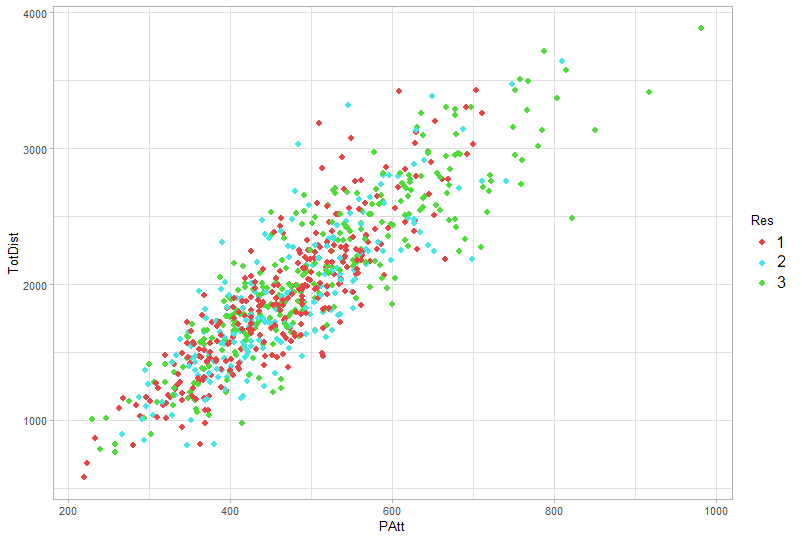
\includegraphics[scale=0.60]{TotDist-PAtt.png}
			\caption{Scatter plot tra \texttt{TotDist} e \texttt{PAtt}}  \label{fig:totdistpatt}
		\end{center}
	\end{figure}
	\item Interazione tra \texttt{TotDist} e \texttt{PCmp\%}. Dato che per poter tentare di effettuare passaggi e completarli è possibile farlo solo se ci si muove con la palla, allora è possibile ipotizzare che vi sia una relazione tra queste variabili. Dalla Figura \ref{fig:totdistpatt} si può notare che tra le due variabili vi è una relazione con correlazione positiva, con una andamento simile a una funzione esponenziale, ciò sarà tenuto conto nella modellazione per valutare se inserire oppure no una delle variabili con un grado superiore.
	\begin{figure}[htbp]
		\begin{center}
			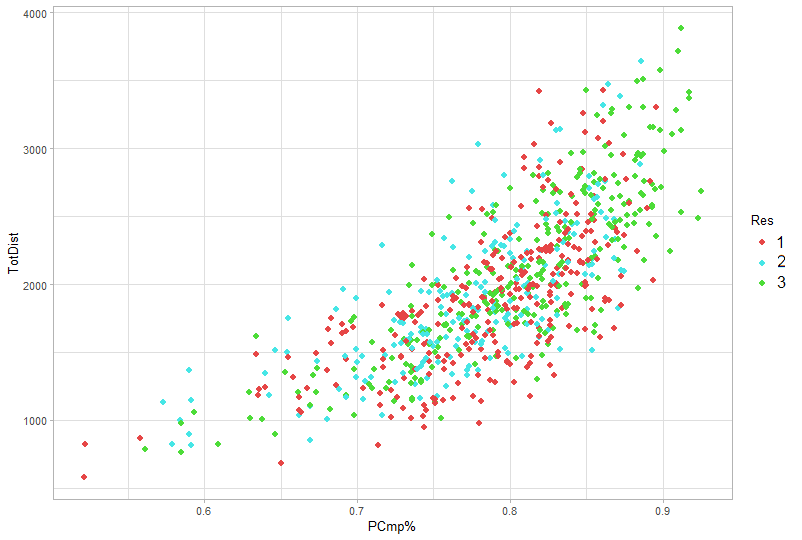
\includegraphics[scale=0.60]{TotDist-PCmp.png}
			\caption{Scatter plot tra \texttt{TotDist} e \texttt{PCmp\%}}  \label{fig:totdistpcmp}
		\end{center}
	\end{figure}
\end{itemize}

Infine sono state individuate le seguenti interazioni:
\begin{itemize}
	\item Interazione tra \texttt{ToAtt3rd} e \texttt{ToAttPen}. Dato che le due variabili si riferiscono a due zone di campo adiacenti e interessanti a fini del l'esito della partita, si ipotizza che vi sia una interazione. Nella Figura \ref{fig:toatt} si può notare un correlazione positiva molto lineare tra le due variabile che prova l'ipotesi. Si nota all'inizio che tutti i dati sono molto vicini ma che via via diventano più sparsi. Tale interazione sembra perciò utile a spiegare la variabile risposta.
	\begin{figure}[htbp]
		\begin{center}
			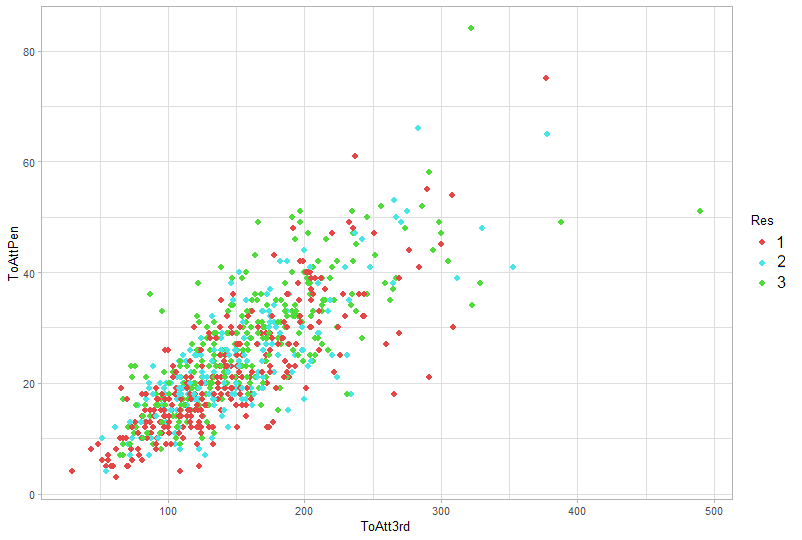
\includegraphics[scale=0.60]{ToAtt3rd-ToAttPen.png}
			\caption{Scatter plot tra \texttt{ToAtt3rd} e \texttt{ToAttPen}}  \label{fig:toatt}
		\end{center}
	\end{figure}
	\item Interazione tra \texttt{PAtt} e \texttt{PCmp\%}. Data la loro naturale correlazione si ipotizza che vi sia una interazione tra loro. Infatti tale interazione è possibile vederla nella Figura \ref{fig:pp} la quale sembra simile alla interazione \texttt{TotDist}*\texttt{PCmp\%}.
	\begin{figure}[htbp]
		\begin{center}
			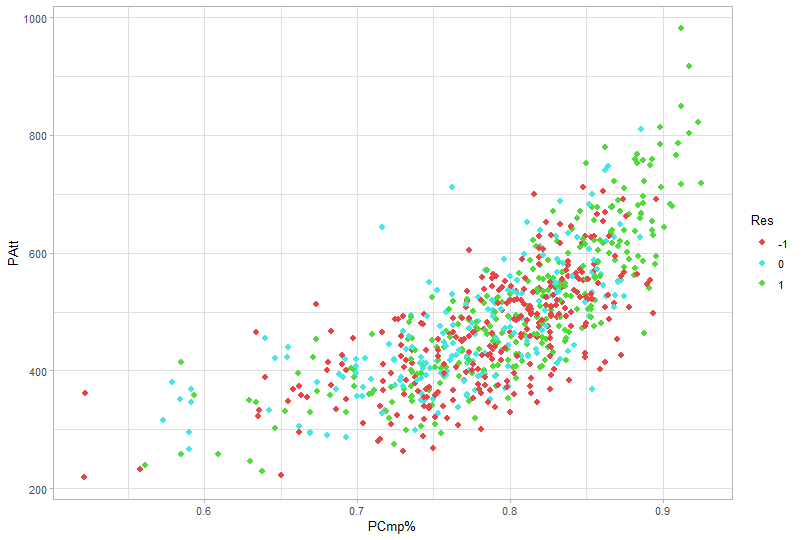
\includegraphics[scale=0.60]{PAtt-PCmp.png}
			\caption{Scatter plot tra \texttt{PAtt} e \texttt{PCmp\%}}  \label{fig:pp}
		\end{center}
	\end{figure}

\end{itemize}

\subsection{Collinearità}
Per collinearità si intende quel fenomeno per il quale se più variabili esplicative altamente correlate vengono inserite nel modello, allora la loro alta correlazione andrà a nasconde la loro associazione con la variabile risposta. La soluzione per risolvere questo problema è quella di scegliere soltanto una sola variabile della relazione da inserire nel modello.\\
Nella Figura \ref{fig:cor} viene mostrato il valore della correlazione per ogni possibile interazione tra variabile numeriche.\\
Come si può notare una maggior correlazione tra le variabile è concentra nella prima parte del triangolo. Dal grafico possiamo vedere come tutte le interazioni che sono state descritte nella sottosezione precedente abbiano un alta correlazione ma non eccessivamente alta. \\
Nella sottosezione precedente si poteva pensare di inserire interazione abbastanza naturali ad esempio: \texttt{PAtt} con \texttt{SPAtt} e con \texttt{MPAtt} e, \texttt{PCmp\%} con \texttt{MPCmp\%} e con \texttt{LPCmp\%}. Tali interazioni pero sono composte da variabili che hanno un alta correlazione tra loro, e quindi si ha il rischio di incombere in un problema di collinearità. In questa fase dell'analisi non si hanno abbastanza elementi per poter scegliere quale variabile tenere e quale no perciò tale scelta verrà rinviata alla fase di modellazione.\\
Infine si nota una buona correlazione tra \texttt{ToDefPen} e \texttt{ToDef3rd}, tale interazione non è stata inserita perché la variabile \texttt{ToDefPen} non è significativa per la variabile risposta.

\begin{figure}[htbp]
	\begin{center}
		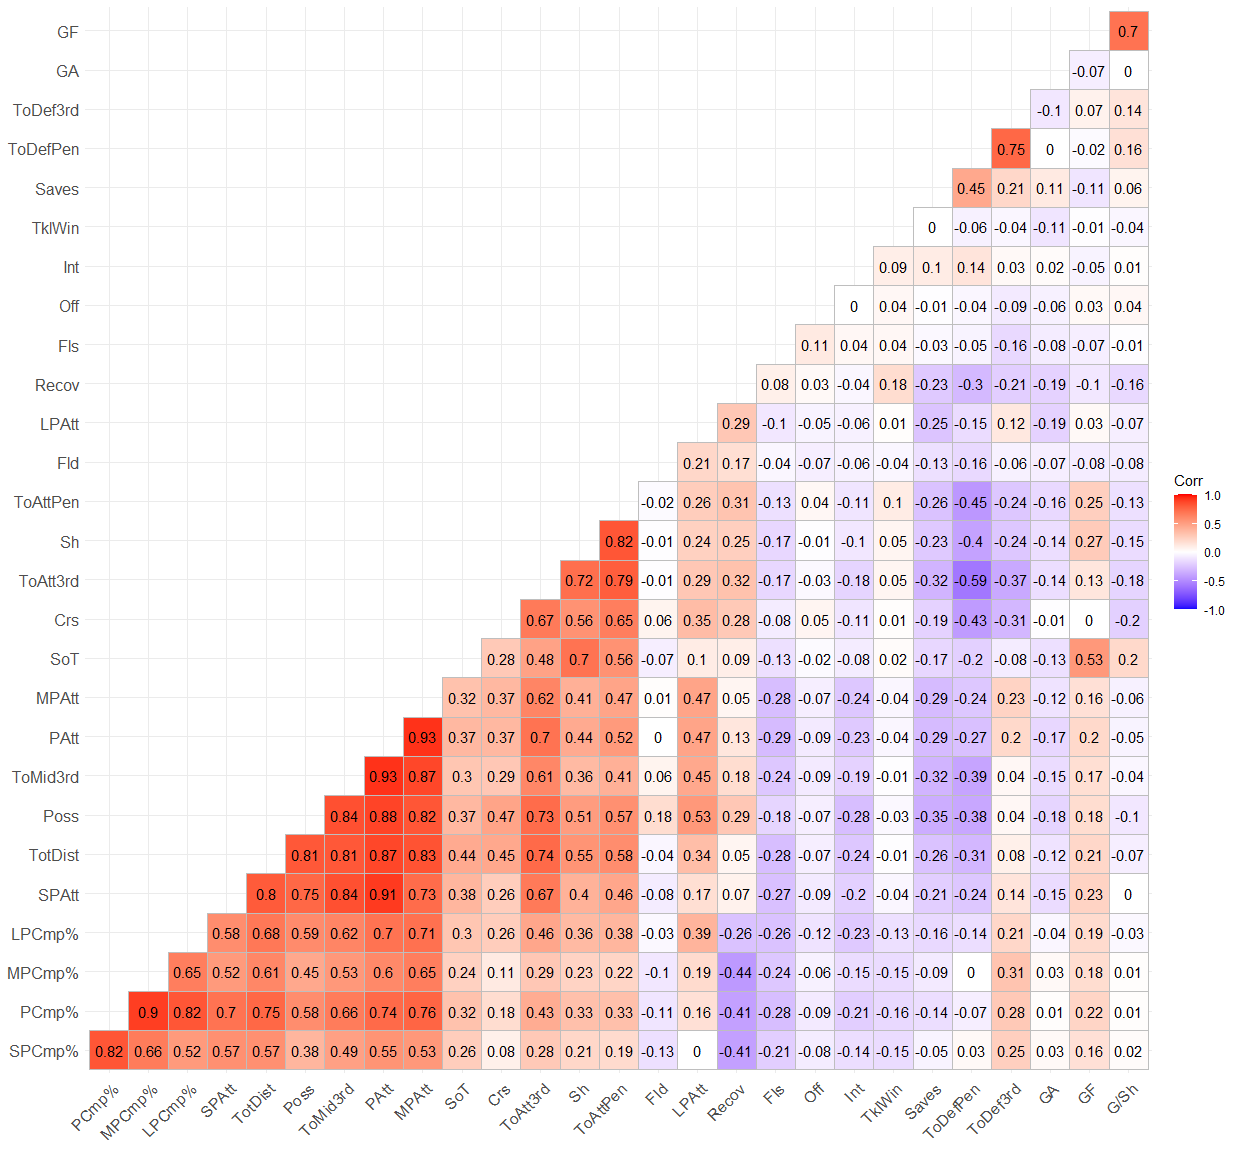
\includegraphics[scale=0.45]{Rplot.png}
		\caption{Grafico delle correlazioni di ogni coppia di variabili}  \label{fig:cor}
	\end{center}
\end{figure}

\begin{figure}[htbp]
	\begin{center}
		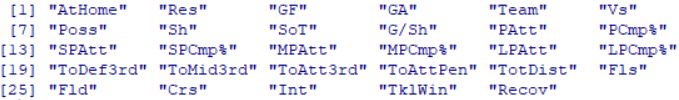
\includegraphics[scale=0.60]{cov.png}
		\caption{Grafico riassuntivo delle variabili rimaste dopo il Prepossesing}  \label{fig:cov}
	\end{center}
\end{figure}

\section{Adattamento dataset al modello}

Nelle sezioni precedenti si è descritto come si è costruito il dataset e come esso è stato strutturato. Tale struttura ha il vantaggio di essere di facile interpretazione per un essere umano ma vi sono alcune criticità che non lo permettono di essere utilizzato correttamente all'interno del modello messo a disposizione dal pacchetto \texttt{BradleyTerry2}.\\ 
Sono state apportare alcune modifiche attraverso la scrittura di codice che andasse a modificare la struttura del dataset in modo da essere correttamente utilizzabile nel modello. \\

Innanzitutto il modello richiede per il suo funzionamento che le due variabili \texttt{Team} e \texttt{Vs} devono essere o di tipo fattore oppure un \textsf{data.frame}. Un \textsf{data.frame} è una lista di vettori, che devono avere tutti la stessa lunghezza, ma possono essere di tipo diverso: variabili nominali cioè fattori, variabili cardinali cioè vettori numerici; un \textsf{data.frame} può essere visto come una matrice ma con il tipo dei valori che può essere diverso.\\ 
Le variabili \textsf{Team} e \textsf{Vs} sono state trasformate in \texttt{data.frame} in modo da poter inserire al loro interno tutte le covariate descritte nella sezione precedente, ad esempio \textsf{Poss}, \textsf{Int} ecc.., cosi che il modello capisca quali valori sono legati alla squadra indicata in \textsf{Team} e quali in \textsf{Vs} nella stessa partita.\\

Inoltre per indicare nel modello se la squadra giocava in casa o no, i valori della variabile \texttt{AtHome} non erano accettati, si è quindi convertito il valore \texttt{TRUE} in 1 mentre FALSE in 0.



\subsection{Codice per l'adattamento del dataset}
Di seguito viene mostrato il codice applicato per adeguare il dataset con le modifiche scritte precedentemente.

\begin{lstlisting}
PossVs <- c()
ShVs <- c()
ShTVs <- c()
G.ShVs <- c()
PAttVs <- c()
PCmp.Vs <- c()
SPAttVs <- c()
SPCmp.Vs <- c()
MPAttVs <- c()
MPCmp.Vs <- c()
LPAttVs <- c()
LPCmp.Vs <- c()
ToDef3rdVs <- c()
ToMid3rdVs <- c()
ToAtt3rdVs <- c()
ToAttPenVs <- c()
ToDistVs <- c()
FlsVs <- c()
FldVs <- c()
CrsVs <- c()
IntVs <- c()
TklWinVs <- c()
RecovVs <- c()
del <-c()
k <- 1
z <- 1
for(i in 1:nrow(soccern)){
  if(soccern$AtHome[i] == TRUE){
	for(j in 1:nrow(soccern)){
		if((soccern$Team[j] == soccern$Vs[i]) && (soccern$Team[i] == soccern$Vs[j]) && (soccern$AtHome[j] == FALSE)){
			PossVs[k] <- soccern$Poss[j]
			ShVs[k] <- soccern$Sh[j]
			ShTVs[k] <- soccern$SoT[j]
			G.ShVs[k] <- soccern$G.Sh[j]
			PAttVs[k] <- soccern$PAtt[j]
			PCmp.Vs[k] <- soccern$PCmp.[j]
			SPAttVs[k] <- soccern$SPAtt[j]
			SPCmp.Vs[k] <- soccern$SPCmp.[j]
			MPAttVs[k] <- soccern$MPAtt[j]
			MPCmp.Vs[k] <- soccern$MPCmp.[j]
			LPAttVs[k] <- soccern$LPAtt[j]
			LPCmp.Vs[k] <- soccern$LPCmp.[j]
			ToDef3rdVs[k] <- soccern$ToDef3rd[j]
			ToMid3rdVs[k] <- soccern$ToMid3rd[j]
			ToAtt3rdVs[k] <- soccern$ToAtt3rd[j]
			ToAttPenVs[k] <- soccern$ToAttPen[j]
			ToDistVs[k] <- soccern$TotDist[j]
			FlsVs[k] <- soccern$Fls[j]
			FldVs[k] <- soccern$Fld[j]
			CrsVs[k] <- soccern$Crs[j]
			IntVs[k] <- soccern$Int[j]
			TklWinVs[k] <- soccern$TklWin[j]
			RecovVs[k] <- soccern$Recov[j]
			k <- k + 1
		}      
	}
  }else{
	 del[z] <- i
	 z <- z + 1
  }
}
\end{lstlisting}
\bigskip

Con il codice precedente si ha l'obbiettivo di prendere le due righe di ogni partita e di unirle insieme formando un unica riga per ogni partita. Successivamente si elimineranno le righe delle partite giocate fuori casa (\textsf{AtHome} = FALSE) dalle squadre indicate in \textsf{Team} mentre le righe delle partite giocate in casa (\textsf{AtHome} = TRUE) dalle squadre indicate in \textsf{Team} conteranno il risultato della fusione.\\
Perciò si è creato un vettore vuoto per ogni covariata presente nel dataset, ad eccezione di \textsf{AtHome} che verrà gestita in un modo diverso. Il vettore \texttt{del} è il vettore che tiene traccia di quali righe saranno da eliminare. \texttt{k} è l'indice usato per scorre il dataset per trovare i dati dell'avversario; \texttt{z} l'indice usato per inserire un nuovo elemento nel vettore \texttt{del}.\\
Il primo ciclo \texttt{for} scorre tutto il dataset alla ricerca delle righe con i dati delle partite giocate in casa dalla squadra indicata in \texttt{Team}, infatti al suo interno il primo costrutto \texttt{if} controlla se la partita è in casa per \texttt{Team} se sì, parte un secondo ciclo \texttt{for} che anche esso scorre tutto il dataset per cercare la riga con la partita giocata della squadra indicata in \texttt{Vs}; giocata ovviamente fuori casa. Perciò all'interno del secondo ciclo \texttt{for} vi è un costrutto \texttt{if} che controlla se la j-esima riga si riferisce alla stessa partita indicata nella i-esima riga, se sì allora si salvano tutti i dati nei vettori e si incrementa l'indice \texttt{k}. Se il primo \texttt{if} da esito negativo allora si andrà a inserire l'indice dell'i-esima riga nel vettore \texttt{del} perché contiene informazioni di una partita giocata fuori casa dalla squadra indicata in \textsf{Team} e viene incrementato l'indice di uno \texttt{z}.\\

Di seguito vengono riportati i comandi fatti per applicare le modifiche al dataset.
\bigskip
\begin{lstlisting}
> soccern3 <- soccern2[-del,]
\end{lstlisting}
\bigskip
\bigskip
Con il precedente commando si va a creare un nuovo dataset con 380 righe, eliminando tutte quelle righe con valore \texttt{FALSE} su \textsf{AtHome}. 
\bigskip
\begin{lstlisting}
> soccern3$Team <- data.frame(team = soccern3$Team, GF = soccern3$GF, GA = soccern3$GA,  at.home = 1, Poss = soccern3$Poss, Sh = soccern3$Sh, SoT = soccern3$SoT, G.Sh = soccern3$G.Sh, PAtt = soccern3$PAtt, PCmp. = soccern3$PCmp., SPAtt = soccern3$SPAtt, SPCmp. = soccern3$SPCmp., MPAtt = soccern3$MPAtt, MPCmp. = soccern3$MPCmp., LPAtt = soccern3$LPAtt, LPCmp. = soccern3$LPCmp., ToDef3rd = soccern3$ToDef3rd, ToAtt3rd = soccern3$ToAtt3rd, ToAttPen = soccern3$ToAttPen, TotDist = soccern3$TotDist, Fls = soccern3$Fls, Fld = soccern3$Fld, Crs = soccern3$Crs, Int = soccern3$Int, TklWin = soccern3$TklWin, Recov = soccern3$Recov)
	
\end{lstlisting}

\bigskip
Con il precedente commando si va a modificare \textsf{Team} rendendolo un \texttt{data.frame}, andando a inserire i dati della riga relativi alla squadra che gioca in casa. Si inserisce come chiave \texttt{team = soccern3\$Team} e si indica che la partita è in casa per la squadra di riferimento con \texttt{at.home = 1}.
\bigskip
\bigskip
\begin{lstlisting}
> soccern3$Vs <- data.frame(team = soccern3$Vs, GF = GFVs, GA = GAVs, at.home = 0, Poss = PossVs, Sh = ShVs, SoT = ShTVs, G.Sh = G.ShVs, PAtt = PAttVs, PCmp. = PCmp.Vs, SPAtt = SPAttVs, SPCmp. = SPCmp.Vs, MPAtt = MPAttVs, MPCmp. = MPCmp.Vs, LPAtt = LPAttVs, LPCmp. = LPCmp.Vs, ToDef3rd = ToDef3rdVs, ToAtt3rd = ToAtt3rdVs, ToAttPen = ToAttPenVs, TotDist = ToDistVs, Fls = FlsVs, Fld = FldVs, Crs = CrsVs, Int = IntVs, TklWin = TklWinVs, Recov = RecovVs)
	
\end{lstlisting}
\bigskip
Con il precedente commando si va a modificare \textsf{Vs} rendendolo un \texttt{data.frame}, andando a inserire i dati della riga relativi alla squadra che gioca fuori casa. Si inserisce come chiave \texttt{team = soccern3\$Vs} e si indica che la partita è fuori casa per la squadra \texttt{Vs} con \texttt{at.home = 0}.\\ Per quanto riguarda il resto dei dati vengo riportati attraverso l'inserimento dei vettori costruiti e riempiti precedentemente.\\
             % Modello BT
%% !TEX encoding = UTF-8
% !TEX TS-program = pdflatex
% !TEX root = ../tesi.tex
%**************************************************************
\chapter{Modeling Paired Comparisons}
%\label{cap:archittettura del sistema AWMS}
%**************************************************************

\intro{Nel seguente capitolo verranno introdotti differenti modelli per la \textit{paired comparisons}, iniziando con il Bradley-Terry model versione standard fino a presentare tutte le sue estensioni usate per l'analisi trattata. }
TO DO

\section{Il Bradley-Terry Model}
Il Bradley-Terry model \autocite{bradley1952rank} asserisce che in una competizione tra due qualsiasi giocatori, detti player \textit{i} e player \textit{j} (i,j $\in$ \{1,...,n\}), la probabilità che \textit{i} sia preferito a \textit{j} è data dal rapporto tra $\alpha_{i}$ e $\alpha_{j}$, dove $\alpha_{i}$ e $\alpha_{j}$ sono parametri che rappresentano la cosiddetta abilità dei due giocatori. Il modello standard non considera covariate e in generale, non presta nessuna attenzione all'eterogeneità causata dai soggetti dei confronti.\\

Formalmente, sia Y$_{i,j}$ la variabile casuale associata al risultato della \emph{paired comparison} tra oggetti \textit{i} e \textit{j}, con \textit{j} > \textit{i} $\in$ \{1,...,n\}, dove nella forma più semplice, il modello dato è il seguente:
\begin{align} 
	P(i\succ j) = P(Y_{i,j} = 1) = \frac{exp(\alpha_{i} - \alpha_{j})}{1 + exp(\alpha_{i} - \alpha_{j})} \label{for:3.1} 
\end{align}

Il modello può essere alternativamente espresso in forma di logit lineare:

\begin{align}
		logit(i \succ j) =  log( \frac{P( i \succ j)}{P( j \succ i))} ) = log(\frac{exp(\alpha_{i})}{exp(\alpha_{j})}) = \alpha_i - \alpha_j 
	\end{align}

La risposta del modello rappresenta la probabilità che un certo oggetto \textit{i} è preferito rispetto su un altro oggetto \textit{j}, $i \succ j$. La variabile Y$_{i,j}$ essendo binaria può assumere solo due valori, Y$_{i,j}$ = 1 se l'oggetto \textit{i} è preferito sull'oggetto j e Y$_{i,j}$ = 0 viceversa. I parametri $\alpha_{n}$ come scritto precedentemente rappresentano l'attrattiva o la forza del loro corrispondente oggetto. Chiaramente questi parametri di abilità devono essere stimati dal modello attraverso la massima verosimiglianza. Infine si noti che vi è necessario un vincolo per identificare i parametri, ad esempio: il vincolo di somma $ \sum_{i=1}^{n} \alpha_{i} = 0 $ oppure il vincolo dell'oggetto di riferimento, $\alpha_{i} = 0$ per un oggetto \textit{i} $\in$ \{1, ..., n\}. Se il vincolo dell'oggetto di riferimento è usato, allora il valore dei parametri abilità degli altri oggetti \textit{j} sarà la differenza rispetto all'oggetto di riferimento \textit{i}.
\\

Si sottolinea inoltre che il modello precedentemente descritto è chiamato modello non strutturato e l'obbiettivo dell'analisi è di fare inferenza sul valore dei parametri abilità $\alpha_{n}$ per stilare una classifica finale di tutti gli oggetti.


\section{Il Bradley-Terry Model con ordered response categories}	
In molti contesti di comparazione tra oggetti, è possibile che sia richiesto di dare una scala di preferenza tra un oggetto e un altro. Supponiamo che due oggetti \textit{i} e \textit{j} siano confrontati e che la preferenza ora non sia più espressa i termini di: preferisco \textit{i} al posto di \textit{j} o viceversa ma, attraverso una scala di preferenza ad esempio, dando una forte preferenza a \textit{i} rispetto a \textit{j} o una leggera preferenza a \textit{i} rispetto a \textit{j} o non dando nessuna preferenza o preferendo leggermente \textit{j} rispetto a \textit{i} oppure preferire fortemente \textit{j} rispetto a \textit{i}. Dal modello descritto nella precedente sezione si passa da due classi di preferenza a cinque classi di preferenza.\\
Ovviamente il caso descritto è di interesse per le comparazioni calcistiche dato che non è sufficiente stimare la probabilità di vittoria o sconfitta ma deve essere obbligantemente preso in considerazione anche il pareggio come risultato. Si necessità perciò di un estensione del classico Bradley-Terry model descritto precedentemente.\\

Modelli che consentono un numero generale di categorie K, sono stati proposti da \autocite{tutz1986bradley} e da \autocite{bradley1952rank}, in particolare quest'ultimo mostrò come due modelli per l'analisi di dati ordinati possono essere adattati per le \emph{ordinal paired comparisons}.\\

Il primo modello è il \emph{cumulative link model} che sfrutta la rappresentazione della variabile casuale latente. In generale, sia H il numero di gradi della scala di preferenza e sia $Z_{i,j}$ una variabile continua casuale latente e siano $\theta_{1} $ < $\theta_{2}$ < .... < $\theta_{H-1}$ le soglie tale che Y$_{i,j} = h$ quando $\theta_{h-1} < Z_{i,j} < \theta_{h}$. Allora:
\begin{align}
	P(Y_{i,j}\leq h) =  \frac{exp(\theta_{h} + \alpha_{i} - \alpha_{j})}{1 + exp(\theta_{h} + \alpha_{i} - \alpha_{j})} \label{for:3.2.1}
\end{align}

con h $\in$ \{1,....,H\} che indica le possibili \emph{response categories}. I parametri $\theta_{h}$ rappresentano le cosiddette soglie per le singole \emph{response categories}, che determinano la preferenza per le specifiche categorie. In particolare, Y$_{i,j} = 1$ rappresenta la massima preferenza per un oggetto \textit{i} rispetto a un oggetto \textit{j}.\\
In generale vi è imposta una simmetria del modello in modo che valga: $P(Y-{i,j} = h) = P(Y_{i,j} = H - h + 1)$. È quindi necessario che le soglie siano ristrette a $\theta_{i}$ = -$\theta_{H-h}$ e se, H è dispari, $\theta_{H/2}$ = 0; per garantire che le probabilità siano simmetriche. Per garantire che le probabilità siano non negative per le singole \emph{response categories} vi è imposta la seguente limitazione: $-\infty$ = $\theta_{0} < \theta_{1} < ... < \theta_{H-1} < \theta_{H} = \infty$. Dato che la soglia per l'ultima categoria è fissata a $\theta_{H} = \infty$ allora vale che $P(Y_{i,j} \leq H)$ = 1. Si sottolinea che le soglie sono parametri che vanno stimate dai dati; inoltre la probabilità di una singola \emph{response category} può essere derivata dalla differenza tra categorie adiacenti cioè:
\begin{center}
	  $P(Y_{i,j} = k)$ = $P(Y_{i,j} \leq h)$ - $P(Y_{i,j} \leq k - 1)$
\end{center}

Il modello delle \emph{adjacent categories model}, così come il modello Bradley-Terry, ha anche una rappresentazione logit lineare ed è il seguente:
\begin{align}
	logit(Y_{i,j}\leq h) =  \theta_{h} + \alpha_i - \alpha_j 
\end{align}

Il secondo modello invece proposto da \autocite{agresti1992analysis} è il \emph{adjacent categories model}. In questo caso il collegamento è applicato alle probabilità di risposte adiacenti, piuttosto che alle probabilità cumulative riducendosi così al modello Bradley-Terry quando sono consentite solo due categorie e al modello proposto da \autocite{davidson1970extending} quando sono consentite solo tre categorie.\\
Il modello proposto da \autocite{davidson1970extending} risulta essere adatto per l'analisi sulle partite di calcio.\\
Il \emph{adjacent categories model} è più semplice da interpretare rispetto ai \emph{cumulative link models} poiché l'odds ratio si riferisce a un determinato risultato anziché a raggruppamenti di risultati. \\
Perciò dal modello proposto da \autocite{davidson1970extending}, sia $\theta$ il parametro stimato dai dati che indica quanto è auspicabile la non preferenza, nel nostro caso il pareggio, allora:

\begin{align}
	P(Y_{i,j} = 2 | Y_{i,j} \not = 0) =  \frac{exp(\alpha_{i} - \alpha_{j})}{1 + exp(\alpha_{i} - \alpha_{j})}, 
\end{align}
	
\begin{align}
	P(Y_{i,j} = 1) =  \frac{\theta \sqrt{exp(\alpha_{i}) * exp(\alpha_{j})}}{exp(\alpha_{i}) + exp(\alpha_{j}) + \theta\sqrt{exp(\alpha_{i}) * exp(\alpha_{j})}}, 
\end{align}

\begin{align}	
	P(Y_{i,j} = 0 | Y_{i,j} \not = 1) =  \frac{exp(\alpha_{j} - \alpha_{i})}{1 + exp(\alpha_{j} - \alpha_{i})}
\end{align}

Come si può vedere si è riportato la modellazione di tutti e tre i possibili risultati, con $\alpha_{n}$ che rappresenta la forza degli oggetti in comparazione da stimare dai dati. La modellazione vittoria e la sconfitta dell'oggetto \textit{i} contro l'oggetto \textit{j} rimane uguale alla modellazione \hyperref[for:3.1]{(3.1)} descritta precedentemente. Diversamente per il pareggio dove viene aggiunto il parametro $\theta$. \\

\section{Il Bradley–Terry Model con variabili esplicative}
Fin ad ora è stato presentato un modello che valutasse il grado di preferenza per un oggetto \textit{i} rispetto a un oggetto \textit{j}, senza che considerasse nessuna variabile. Chiaramente tale modello risulta essere inutile per le nostre analisi, dato che siamo interessati a capire quali variabili possono influenzare il risultato della comparazione. Si necessita perciò di un modello che tenga conto anche di variabili esplicative inserite durante l'analisi. \\
Sia x$_{i}$=($x_{i1},....x_{iK}$) il vettore di K variabili esplicative per un certo oggetto \textit{i} e $\beta$ = ($\beta_{1},....\beta_{P}$) il vettore dei pesi stimati per ogni variabile presente in x$_{i}$, allora si ha che il parametro abilità $\alpha_{i}$ di un certo oggetto \textit{i} è uguale a:

\begin{center}
	\begin{large}
	 $\alpha_{i}$ = $\beta_{1}x_{i1}$ + .... + $\beta_{P}x_{iP}$      con i=1,....,n
	\end{large}

\end{center}

Si ha quindi che il parametro abilità $\alpha_{i}$ per un certo oggetto \textit{i} è una combinazione lineare di variabili.\\
Il modello è stato presentato per la prima volta da \autocite{springall1973response}; tale modello viene chiamato modello strutturato.\\
 
Grazie a questo modello se vi sono covariate che hanno un legame con la variabile risposta, tanto da influenzarne l'esito con quest'ultima allora, sarà possibile inserirle nel modello. Nel caso calcistico tali covariate possono essere il possesso della palla o il numero di falli fatti.


\subsection{Il Bradley–Terry Model con effetto partite in casa}
Nel modello descritto nella sezione 2.2, si era scritto che, era necessario imporre la simmetria tra le categorie di risposta. Purtroppo la simmetria imposta risulta essere non adeguata in alcuni contesti, tra questi vi è anche il calcio; poiché l'ordine dei oggetti conta. Infatti nel calcio la prima squadra che viene indicata tra le due squadre, è quella che gioca in casa, dove teoricamente dovrebbe avere un vantaggio sull'avversario. Perciò, il presupposto che le categorie di risposta siano simmetriche non vale più. \\
Un possibile modello riadattato al problema esposto è il seguente:

\begin{align} 
	P(i\succ j) = P(Y_{i,j} = 1) = \frac{exp(\delta + \alpha_{i} - \alpha_{j})}{1 + exp(\delta + \alpha_{i} - \alpha_{j})} \label{for:3.8} 
\end{align}

Il qual'è il modello \hyperref[for:3.1]{(3.1)} riadatto e da cui possiamo derivare il modello \hyperref[for:3.2.1]{(3.3)} riadatto che è il seguente:

\begin{align}
	P(Y_{i,j}\leq h) =  \frac{exp(\delta + \theta_{h} + \alpha_{i} - \alpha_{j})}{1 + exp(\delta + \theta_{h} + \alpha_{i} - \alpha_{j})} \label{for:3.9}
\end{align}

Come si può vedere il vantaggio di giocare in casa, in generale l'effetto d'ordine; viene trattato come una variabile esplicativa. Infatti se $\delta$ > 0 allora viene attribuito un vantaggio all'oggetto \textit{i}, nel contesto calcistico significa che gioca in casa; aumentando la probabilità che vinca il confronto o nel caso di \emph{ordered response categories}, di avere un risultato superiore rispetto all'oggetto \textit{j}. Chiaramente il peso di $\delta$ deve essere stimato dai dati.\\

Il modello \hyperref[for:3.8]{(3.8)} cosi come il modello \hyperref[for:3.9]{(3.9)} , hanno anche una rappresentazione logit lineare e sono le seguenti:\\

Per \hyperref[for:3.8]{(3.8)}

\begin{align}
	logit(i \succ j) =  \delta + \alpha_i - \alpha_j 
\end{align}

Per \hyperref[for:3.9]{(3.9)}

\begin{align}
	logit(Y_{i,j}\leq h) =  \delta + \theta_{h} + \alpha_i - \alpha_j 
\end{align}
	             % 
%% !TEX encoding = UTF-8
% !TEX TS-program = pdflatex
% !TEX root = ../tesi.tex

%**************************************************************
\chapter{Risultati dei modelli Bradley-Terry}
\label{cap:risultatiDM}
%**************************************************************

\intro{In questo capitolo vengono presente le stime e i risultati ottenuti dai modelli Bradley-Terry (BTM) presentati nel Capitolo \ref{cap:BT}. Inoltre, sarà riportata l'applicazione del metodo  \emph{LASSO} con relativi risultati. Infine si riporteranno le predizioni sugli esiti delle partite prodotte dai modelli per essere poi confrontate con le predizioni dei \emph{bookmakes}}\\
 %Seguirà poi un analisi conclusiva sulle variabile esplicative alla luce dei risultati ottenuti.
\section{Premesse}
I risultati che verranno esposti non tengono in considerazione le variabili esplicative del numero di gol fatti \texttt{GF} e dei gol subiti \texttt{GA}. Questo perché provocano la non convergenza del modello. Inoltre data l'elevata complessità che raggiunge il modello esteso Bradley-Terry, non sono state inserite le interazioni illustrate nel Capitolo \ref{cap:Analisi}.

\section{BTM con effetto dell'ordine}
Le analisi dello studio iniziano con l'applicazione del modello \hyperref[for:3.9]{(4.9)}. Tale modello è abbastanza semplice, infatti la stima dell'abilità delle squadre tiene conto solo degli esiti osservarti delle varie partite e del vantaggio di giocare in casa. Ovviamente da tali stime si basa la distribuzione di probabilità degli esiti delle partite.\\
La stima dei parametri soglia $\theta_1$ e $\theta_2$ sono rispettivamente di -0.669 e 0.669 mentre il parametro $\delta$ globale per tutte le squadre è di 0.099 con uno \emph{standard error} (SE) di 0.126. Si nota che il vantaggio di giocare in casa effettivamente è un vantaggio anche secondo il modello, infatti la stima del parametro è positiva, quindi generalmente ha un effetto positivo per la squadra in casa. Nella Tabella \ref{tab:BTH} vengono riportati i risultati ottenuti in ordine dell'abilità stimata.\\
	\begin{table}[!htb]%
	
	\renewcommand{\arraystretch}{1.7}
	\centering
	\begin{tabular}{c c c c c c}
		\hline	
		
		\textbf{Squadra} & \textbf{Abilità} & \textbf{SE} & \textbf{QSE} & \textbf{QV} & \textbf{Rank}   \\	
		\hline			
		Milan & 1.492 & 0.557 & 0.359 & 0.129 & 1\\
		Inter & 1.4 & 0.537 & 0.400 & 0.160 & 2\\
		Napoli & 1.17 & 0.530 & 0.389 & 0.152 & 3 \\
		Juventus & 0.825 & 0.520& 0.373& 0.139& 4\\
		Lazio & 0.459 & 0.516 & 0.368 & 0.135 & 5\\
		Roma & 0.413 & 0.516& 0.368& 0.135& 6\\
		Fiorentina & 0.339 & 0.511& 0.357& 0.127& 7\\
		Atalanta & 0.312 & 0.000 & 0.368& 0.135& 8 \\
		Hellas Verona & 0.049 & 0.513& 0.356& 0.127& 9\\
		Torino & -0.012 & 0.512 & 0.355& 0.126& 10 \\
		*Udinese & -0.072 & 0.512& 0.355 & 0.126& 12\\
		*Sassuolo & -0.145 & 0.511& 0.355 & 0.126& 11\\
		Bologna & -0.233 & 0.515& 0.359& 0.128& 13\\
		Empoli & -0.549 & 0.518& 0.362& 0.131& 14\\
		Sampdoria & -0.775 & 0.527& 0.372& 0.138& 15\\
		Spezia & -0.831 & 0.527& 0.372& 0.138& 16\\
		*Genoa & -0.879 & 0.532& 0.378& 0.143& 19 \\
		Cagliari & -0.897 & 0.532& 0.378& 0.143& 18\\
		*Salernitana & -0.91 & 0.527& 0.372& 0.138& 17\\
		Venezia & -1.156 & 0.538& 0.387& 0.149& 20\\
		\hline
		& & & & &\\
		
	\end{tabular} \hbox{}
	
	\caption{Per ogni squadra viene riportata l'abilità stimata, lo \emph{Standard 
		Error} (SE), il \emph{Quasi Standard Error} (QSE) e il \emph{Quasi Variance} (QV).} \label{tab:BTH}
\end{table}
Nonostante, la semplicità del modello, viene offerta una stima delle abilità delle squadre che rispecchia molto il piazzamento mostrato nella Tabella \ref{tab:ranking}. Infatti, solo quattro squadre hanno un piazzamento diverso da quello reale. L'Udinese e il Sassuolo hanno il piazzamento invertito con una stima dell'abilità che è molto simile. Ciò è un bene dato che nella stagione in esame il loro distacco è stato solo di tre punti. Anche Genoa e Salernitana hanno un piazzamento differente da quello reale. Per quanto riguarda il Genoa tale risultato può essere spiegato dal fatto che all'inizio del campionato ha avuto un buon andamento (vedi \textit{\cite{storyGenoa}}) e dall'ottenimento di punti contro Juventus, Inter, Roma e Atalanta, cioè squadre considerate tra le più forti del campionato. Per quanto la stima al ribasso della Salernitana è determinata dal suo pessimo andamento per la maggior parte del campionato fatta eccezione per l'ultima parte, dove sono stati guadagnati la maggior parte dei punti, tanto da permettere alla squadra di guadagnare all'ultima giornata la salvezza (vedi \textit{\cite{storySal}}). \\
Come si può notare oltre allo \emph{Standard Error} (SE) sono state riportate altre due misurazioni, il \emph{Quasi Standard Error} (QSE) \autocite{firth2004quasi} e il \emph{Quasi Variance} (QV)\autocite{firth2004quasi}. Il \emph{Quasi Variance} (QV)\autocite{firth2004quasi} è un metodo che fornisce un'approssimazione della varianza, ed è utilizzato per confrontare livelli differenti di un fattore. Il tipo fattore è stato illustrato nel Capitolo \ref{cap:Analisi}. Il QV è stato introdotta da \textcite{firth2004quasi} per risolvere il problema della categoria di riferimento. Tale problema si riferisce al fatto che risulta essere semplice confrontare un livello qualsiasi del fattore con il suo livello di riferimento ma confrontare tra loro due livelli entrambi non di riferimento non è possibile. Grazie a il QV cioè è possibile, infatti permette di confrontare tra di loro diversi livelli che non sono di riferimento con il vantaggio di non dover riportare tutta la matrice delle varianze e delle covarianze per effettuare i confronti. Nel nostro caso abbiamo la variabile \texttt{team} di tipo fattore con la squadra Atalanta come livello di riferimento. Grazie al QV ci viene fornita il QSE, una stima dello SE che verrà utilizzata per confrontare le abilità stimate dei diversi livelli, ovvero le squadre, per poter dedurre se la differenza di abilità tra due squadre è significativa dal punto di vista statistico. Con il QSE le squadre vengono trattate come variabili indipendenti. Esempio di applicazioni del QSE e del QV su BTM è possibile trovarli in \textcite{firth2004quasi} e in \textcite{turner2012bradley}.\\
Perciò, confrontiamo le stime dei valori delle abilità delle squadre classificatesi nelle prime due posizione, rispettivamente Milan e Inter. Il QSE per il Milan è di 0.359 mentre per l'Inter è di 0.400. La differenza tra le loro abilità è di |1.492 - 1.4| = 0.092. Applicando il calcolo pitagorico è possibile calcolare lo QSE, cioè un SE approssimato, relativo alla differenza tra abilità, e quindi ($0.359^2 + 0.400^2)^\frac{1}{2}=0,537 > 0.092$. Perciò la differenza in termini di abilità tra le due squadre non è significativa da un punto di vista statistico. Infatti le due squadre hanno un differenza di soli due punti.
%**************************************************************

\section{BTM con covariate specifiche dell'oggetto}
In questa sezione si andrà ad aggiungere al modello Bradley-Terry le variabili esplicative, presentandone i risultati. Il modello applicato è il seguente
\begin{align}
	P(Y_{p(i,j)}\leq k) =  \frac{exp(\delta + \theta_{k} + \beta_{i0} - \beta_{j0} + x^T_{pi}\tau - x^T_{pj}\tau)}{1 + exp(\delta + \theta_{k} + \beta_{i0} - \beta_{j0} + x^T_{pi}\tau - x^T_{pj}\tau)}, \label{for:5.1}
\end{align}
dove l'effetto dell'ordine $\delta$, cioè il vantaggio di giocare la partita in casa, ha ancora un effetto globale per tutte le squadre, mentre $x^T_{pi}$ è il vettore con tutti i valori delle ventisei covariate per l'i-esima squadra e per la p-esima partita. Il parametro $\tau$ è il peso medio stimato di ogni covariata. Le covariate perciò sono specifiche del soggetto e dell'oggetto ma con un effetto specifico dell'oggetto.\\
La stima dei parametri soglia $\theta_1$ e $\theta_2$ sono rispettivamente di -1.113 e 1.113 mentre il parametro $\delta$ globale per tutte le squadre è salito a 0.27 con uno SE di 0.142. Nella Tabella \ref{tab:BTC} e nella Tabella \ref{tab:BTC2} vengono riportate le stime delle abilità delle squadre con i relativi SE, QSE e QV, e le stime di ogni covariata sul modello con relativo SE.\\
\begin{table}[!htb]%
	
	\renewcommand{\arraystretch}{1.7}
	\centering
	\begin{tabular}{c c c c c c}
		\hline	
		
		\textbf{Squadra} & \textbf{Abilità} & \textbf{SE} & \textbf{QSE} & \textbf{QV} & \textbf{Rank}   \\	
		\hline			
		Milan & 1.406 & 0.644 & 0.455 & 0.239 & 1\\
		Inter & 1.097 & 0.685 & 0.433 & 0.286 & 2\\
		Napoli & 1.067 & 0.595 & 0.423 & 0.236 & 3 \\		
		Juventus & 0.892 & 0.623 & 0.417& 0.226& 4\\
		Lazio & 0.399 & 0.645 & 0.467 & 0.276 & 5\\
		Roma & 0.377 & 0.634 & 0.469 & 0.279 & 6\\
		*Atalanta & 0.317 & 0.000 & 0.423& 0.238& 8 \\
		*Fiorentina & 0.236 & 0.596 & 0.383 & 0.235& 7\\
		*Torino & 0.092 & 0.591 & 0.427 & 0.165 & 10 \\
		*Hellas Verona & 0.013 & 0.561 & 0.427& 0.164& 9\\
		Sassuolo & -0.023 & 0.587 & 0.435 & 0.253& 11\\
		*Bologna & -0.045 & 0.657& 0.459& 0.128& 13\\
		*Empoli & -0.094 & 0.618& 0.432& 0.211 & 14\\
		*Udinese & -0.178 & 0.642& 0.478 & 0.281& 12\\
		Sampdoria & -0.426 & 0.600 & 0.453& 0.288& 15\\
		*Salernitana & -0.854 & 0.544& 0.429& 0.219& 17\\
		*Spezia & -0.922 & 0.587& 0.452 & 0.249 & 16\\
		Cagliari & -1.01 & 0.612 & 0.498& 0.269 & 18\\
		Genoa & -1.026 & 0.632 & 0.456 & 0.214& 19 \\
		Venezia & -1.318 & 0.592 & 0.434 & 0.231 & 20\\
	
		\hline
		& & & & & \\
		
	\end{tabular} \hbox{}
\caption{Stime delle abilità con relativi \emph{Standard 
		Error} (SE), \emph{Quasi Standard Error} (QSE) e \emph{Quasi Variance} (QV).} \label{tab:BTC}  
\end{table}

\begin{table}[]%
	
	\renewcommand{\arraystretch}{1.7}
	\centering
	\begin{tabular}{c c c }
		\hline	
		
		\textbf{Covariata} & \textbf{Stima} & \textbf{SE} \\	
		\hline
		ToMid3rd & 1.57 & 0.025\\
		G/Sh & 1.135 & 0.317 \\
		Sh & 0.787 & 0.085 \\  
		SoT &  0.536 & 0.324 \\  
		PCmp\% & 0.534 & 0.300 \\
		ToDefPen & 0.375 & 0.027 \\      
		ToDef3rd & 0.347 & 0.026 \\
		ToAtt3rd & 0.283 & 0.025 \\     	     	 
		Saves & 0.280 & 0.312 \\ 
		Fls & 0.138 & 0.204  \\     
		Fld & 0.100 & 0.204  \\
		TklWin &  0.082 & 0.049  \\    
		LPAtt & 0.078 & 0.049  \\ 		
		Poss & 0.032 & 0.169 \\ 
		ToAttPen & 0.027 & 0.044 \\  
		TotDist & -0.039 & 0.001 \\  	
		Off & -0.054 & 0.144  \\
		PAtt & -0.080 & 0.053 \\ 
		Int & -0.082 & 0.057 \\  
		SPCmp\% & -0.100 & 0.136 \\ 
		Crs & -0.199 & 0.062\\  
		LPCmp\% & -0.309 & 0.380 \\ 
		Recov &  -0.512 & 0.030 \\        
		SPAtt & -0.650 & 0.053 \\     
		MPCmp\% & -0.748 & 0.126 \\
		MPAtt & -1.011 & 0.050 \\     		     		   		    
		\hline
		& &  \\
		
	\end{tabular} \hbox{}
\caption{Stime delle covariate con relativo \emph{Standard 
		Error} (SE).} \label{tab:BTC2} 
     
\end{table}

Nella stima dei parametri delle variabili esplicative, ci sono alcune di essi che hanno un forte legame con l'esito della partita, mentre altre quasi nullo. Per le covariate con un forte legame si può distinguere tra chi ha un peso positivo e che quindi incentiva all'ottenimento della vittoria, e chi invece l'opposto, cioè l'ottenimento della sconfitta a causa di effetto negativo.\\
Come ci si aspetta le variabili esplicative legate ai tiri quindi, tiri \texttt{Sh}, tiri in porta \texttt{SoT} e il rapporto tiri/gol \texttt{G/Sh} hanno un peso stimato molto alto e positivo. Sono perciò fortemente decisive per aumentare la probabilità di vittoria. Da notare che sia \texttt{G/Sh} e sia \texttt{Sh} hanno un alto SE, tra i più alti tra i SE delle stime, c'è quindi un elevata variabilità. Sarà interessante perciò analizzare nel prossimo modello, che peso hanno queste covariate per ogni singola squadra data la loro alta variabilità.\\
Sorprendentemente la variabile esplicativa che ha il peso più determinate nell'aumentare le probabilità di vittoria è il numero di tocchi con la palla fatti a centrocampo \texttt{ToMid3rd}. Invece, le altre covariate legate ai tocchi nelle altre zone dal campo quindi \texttt{ToDefPen}, \texttt{ToDef3rd}, \texttt{ToAtt3rd} e \texttt{ToAttPen} hanno comunque un peso positivo ma molto minore rispetto a \texttt{ToMid3rd}. Sembra perciò avere il controllo del centrocampo sia fondamentale per costruire azioni da gol ma anche per mantenere un risultato positivo dalla partita, anzi mantenere il pallone in zone difensive con meno transizioni in zone d'attacco sembra che dia maggior probabilità di vittoria. Infatti, si può notare che un elevato numero di tocchi in area di rigore avversaria \texttt{ToAttPen} aumenti di molto poco la probabilità di vittoria. Infatti, solitamente il campionato italiano è spesso considerato un campionato difensivista e tattico (vedi \textit{\cite{speculazione}}), dove si spinge l'avversario a sbilanciarsi per poi attaccarlo in contropiede.\\
Un aspetto difensivo chiave sembra essere le parate fatte \texttt{Saves}. Inoltre, anche il numero di contrasti vinti \texttt{TklWin} pare abbia un effetto positivo sulla vittoria. Sorprendentemente però per quanto riguarda le altre variabili esplicative difensive rispettivamente, numero di intercetti \texttt{Int} e numero di recuperi \texttt{Recov} hanno un effetto negativo sulla probabilità di vittoria. \\
Al contrario di quanto si pensi il possesso della palla non sembra essere un elemento chiave per la vittoria. Infatti il sua stima fa aumentare di molto poco la probabilità di vittoria. Analogamente anche la distanza percorsa con la palla \texttt{TotDist} non sembra essere un elemento chiave per la vittoria anzi va a diminuire la probabilità di vittoria. Perciò sembra che stia emergendo dall'analisi una tendenza ad avere il controllo del gioco nei momenti giusti e nelle zone giuste del campo per aver maggior probabilità di vittoria.\\
Per quanto riguarda l'aggressività della squadra, sembra che commettere falli  \texttt{Fld} aumenti le probabilità di vittoria, d'altra parte subire falli \texttt{Fls} è più conveniente.\\ 
Si nota che subire un fuorigioco \texttt{Off} ha un impatto negativo sulle probabilità di vittoria.\\
Per quanto riguarda le covariate legate ai passaggi notiamo che solo la percentuale dei passaggi completati \texttt{PCmp\%} e il numero di lanci lunghi tentati \texttt{LPAtt} aumentano le probabilità di vittoria, le restanti covariate invece hanno ne diminuiscono la probabilità. Sembra perciò che un abuso di passaggi filtrati \texttt{MPAtt} o di cross \texttt{Crs} sia controproducente per la vittoria, al contrario avere una buona precisione in generale sui passaggi \texttt{PCmp\%} e effettuare cambi di gioco da maggiori probabilità di vittoria \texttt{LPAtt}. \\

Come fatto nella sezione precedente è possibile anche qui confrontare tra loro le squadre utilizzando i loro QSE relativi alla loro abilità stimata.
Confrontando ancora le prime due squadre, calcolando la loro differenza di abilità, |1.406 - 1.097| = 0.309 e il relativo QSE ($0.455^2 + 0.433^2)^\frac{1}{2}=0,628 > 0.309$, si ottiene che, la differenza di abilità tra le due squadre è ancora non significativa anche con l’effetto delle covariate.

\section{BTM e LASSO}
Nella sezione precedente si sono presentati i risultati ottenuti di un modello Bradley-Terry con l'inserimento di covariate con effetto specifico dell'oggetto. È però di interesse per le nostre analisi capire come ogni singola covariata sia determinante per la vittoria asseconda della squadra in esame. Per esempio, è possibile che il possesso della palla possa essere determinate per una squadra mentre per un'altra no. A tale scopo si applicherà il modello (\ref{for:4.9}) utilizzando covariate specifiche del soggetto e dell'oggetto. Ovviamente con l'inserimento di questo tipo di covariate il modello sarà estremante complesso, infatti avrà 520 covariate. Di conseguenza sarà applicata una selezione delle covariate operata attraverso il metodo \emph{LASSO} illustrato nel Capitolo \ref{cap:BT}. Sempre attraverso il \emph{LASSO} sarà di interesse individuare clusters di squadre che per una certa covariata hanno un effetto simile. Allo stesso tempo si cercherà di individuare quali squadre invece si discostano maggiormente da questi clusters.\\
Purtroppo non è stato possibile riportare gli SE delle stime a causa dell'elevata complessità del procedimento di calcolo. Infatti per calcolare gli SE delle stime è possibile solo farlo attraverso la procedura di tipo \emph{bootstrap} \autocite{henderson2005bootstrap}. Purtroppo però è molto onerosa in termini di computazione, soprattutto con un numero elevato di covariate.\\
Nella Tabella \ref{tab:BTCL}, Tabella \ref{tab:BTCL2} e nella Tabella \ref{tab:BTCL3} vengono riportate le stime dei parametri delle abilità e delle covariate per ogni singola squadra. Si noti che, non tutte le covariate hanno un’unica stima per tutte le squadre, ma in alcuni casi, ci sono più stime per alcune covariate. Perciò per ogni stima del parametro di una covariata verrà indicata quale squadra ha tale valore stimato. Nell'analisi dei risultati spesso si farà un confronto con i risultati ottenuti con il modello della sezione precedente.\\

\begin{table}[!htb]%
	
	\renewcommand{\arraystretch}{1.7}
	\centering
	\begin{tabular}{c c c }
		\hline	
		
		\textbf{Squadra} & \textbf{Abilità} & \textbf{Rank}   \\	
		\hline			
		Milan & 1.673 & 1\\
		Inter & 1.443 &  2\\
		Napoli & 1.436 & 3 \\		
		Juventus & 1.003 & 4\\
		Lazio & 0.641 & 5\\
		*Atalanta & 0.594 & 8 \\
		*Roma & 0.555 &  6\\
		*Fiorentina & 0.227 &  7\\
		Hellas Verona & 0.126 & 9 \\
		Torino & -0.042 & 10 \\	
		Sassuolo & -0.171 & 11\\
		Udinese & -0.262 & 12\\
		Bologna & -0.292 &  13\\
		Empoli & -0.386 & 14\\
		*Spezia & -0.869 &  16\\
		*Salernitana & -0.876 & 17\\
		*Sampdoria & -1.095 &  15\\
		Cagliari & -1.136 &  18\\
		Genoa & -1.231 & 19 \\
		Venezia & -1.338 &  20\\
		
		\hline
		& &  \\
		
	\end{tabular} \hbox{}
	\caption{Stime delle abilità per ogni squadra.} \label{tab:BTCL}  
\end{table}

\begin{table}[]%
	
	\renewcommand{\arraystretch}{1.7}
	\centering
	\begin{tabular}{ccp{10cm}}
		\hline	
		
		\textbf{Covariata} & \textbf{Stima} & \textbf{Squadra} \\	
		\hline
		Home & 0.310 & Tutti\\
		Poss & 0.239 & Lazio \\
		Poss & 0.171 & Torino\\
		Poss & 0.000 & Tutti tranne Lazio e Torino\\
		Sh & 0.520 & Tutti \\
		SoT & 0.596 & Atalanta, Cagliari, Empoli, Genoa, Verona, Juventus, Lazio, Milan, Napoli, Salernitana, Sampdoria, Sassuolo, Spezia, Torino, Venezia\\
		SoT & 0.495 & Inter, Roma \\
		SoT & 0.361 & Bologna \\
		SoT & 0.263 & Fiorentina\\
		SoT & 0.007 & Udinese \\
		G/Sh & 1.107 & Tutti \\
		Saves & 0.260 & Tutti \\
		PAtt & 0.000 & Tutti \\
		PCmp\% & 0.000 & Tutti \\
		SPAtt & 0.124 & Napoli \\
		SPAtt & 0.000 & Tutti tranne Napoli \\
		SPCmp\% & 0.067 & Tutti tranne Genoa \\ 
		SPCmp\% & -0.235 & Genoa \\	
		MPAtt & -0.058 & Tutti \\ 
		MPCmp\% & -0.246 & Tutti tranne Bologna e Genoa \\
		MPCmp\% & -0.255 & Bologna e Genoa \\
		LPAtt & 0.077 & Tutti \\
		LPCmp\% & 0.199 & Hellas Verona \\
		LPCmp\% & 0.000 & Tutti tranne Bologna e Verona \\
		LPCmp\% & -0.303 & Bologna \\	     		   		    
		\hline
		& &  \\
		
	\end{tabular} \hbox{}
	\caption{Stime delle covariate.} \label{tab:BTCL2} 
	
\end{table}
\begin{table}[]%
	
\renewcommand{\arraystretch}{1.7}
\centering
\begin{tabular}{ccp{10cm}}
	\hline			
	\textbf{Covariata} & \textbf{Stima} & \textbf{Squadra} \\	
	\hline
	ToDefPen & 0.135 & Tutti \\      
	ToDef3rd & 0.000 & Tutti \\
	ToMid3rd & 0.147 &Tutti\\
	ToAtt3rd & -0.154 & Tutti \\  
	ToAttPen & 0.000 & Tutti tranne Atalanta \\    
	ToAttPen & -0.311 & Atalanta \\ 	     	 
	TotDist & 0.000 & Tutti \\	
	Fls & 0.219 & Bologna  \\
	Fls & 0.012 & Tutti tranne Bologna, Napoli, Genoa e Salernitana  \\ 		
	Fls & -0.001 & Napoli  \\
	Fls & -0.030 & Genoa, Salernitana  \\
	Fld & 0.100 & Spezia \\
	Fld & 0.015 & Tutti tranne Spezia e Udinese  \\
	Fld & -0.005 & Udinese \\
	Off & 0.055 & Hellas Verona\\
	Off & 0.002 & Tutti tranne Verona, Inter, Juventus, Milan e Napoli\\
	Off & -0.097 & Inter, Juventus, Milan e Napoli  \\
	Crs & 0.000 & Torino\\
	Crs & -0.180 & Tutti tranne Milan, Roma, Torino, Atalanta e Napoli\\
	Crs & -0.391 & Milan e Roma\\
	Crs & -0.671 & Atalanta e Napoli\\
	Int & 0.012 & Tutti\\
	TklWin &  0.225 & Empoli  \\
	TklWin &  0.086 & Tutti tranne Empoli  \\ 
	Recov &  -0.132& Tutti tranne Udinese \\ 
	Recov &  -0.189& Udinese \\ 
\hline
& &  \\

\end{tabular} \hbox{}
\caption{Stime delle covariate.} \label{tab:BTCL3} 
\end{table}

Nella Tabella \ref{tab:BTCL} si può notare che le abilità stimate sono quasi sempre  in linea con il piazzamento reale, risultando migliore rispetto al modello precedente. Purtroppo l'Atalanta viene sovrastimata nonostante al termine della stagione si sia classificata dietro a Roma e Fiorentina. Tale fenomeno può essere spiegato dal fatto che l'Atalanta per larga parte della stagione militasse tra il terzo e il quarto posto, ma nell'ultima parte della stagione l'Atalanta è crollata di prestazione (vedi \textit{\cite{storyAta}}). Si nota che la Sampdoria viene sottostimata, probabilmente perché non ha fatto una buona stagione in generale e verso fine campionato ha avuto un crollo di prestazioni (vedi \textit{\cite{storySamp}}).\\

Nella Tabella \ref{tab:BTCL2} e nella Tabella \ref{tab:BTCL3} alcune variabili esplicative sono state porta a zero, quindi eliminate, mentre altre hanno diversi valori a seconda della squadra in considerazione. \\
Tra le covariate eliminate c'è il numero di passaggi tentati \texttt{PAtt} che nella Tabella \ref{tab:BTC2} del modello precedente aveva un valore stimato quasi nullo oltre a un SE basso. Sorprendentemente anche la percentuale di passaggi tentati \texttt{PCmp\%} viene eliminata dal modello nonostante per il modello precedente avesse un valore alto stimato del parametro. Anche il numero di tocchi nella trequarti di difesa \texttt{ToDef3rd} viene tolta dal modello nonostante un valore stimato alto nella Tabella \ref{tab:BTC2}, ma aveva un bassissimo SE. Infine l'ultima variabile esplicativa eliminata interamente del modello è la distanza percorsa con la palla \texttt{TotDist} rimanendo in linea con quanto visto nella \ref{tab:BTC2} dove \texttt{TotDist} aveva sia una stima del parametro e sia un SE bassissimi.\\
Anche qui viene confermato che giocare la partita \texttt{Home} ha un effetto positivo stimato in 0.310.\\
Per quanto riguarda invece il possesso della palla \texttt{Poss}, come ci si attende dallo scorso modello, viene stimato con un peso nullo per la maggior parte delle squadre ad eccezione di Lazio e Torino dove ha un effetto positivo. Il risultato della stima legata alla Lazio è un risultato in realtà non è sorprendente, infatti il \textit{\cite{sarrismotr}} neologismo per indicare il gioco applicato dall'allenatore Maurizio Sarri, allenatore della Lazio nella stagione 2021/2022, ha tra le sue caratteristiche il mantenimento del possesso della palla, oltre a una propensione offensiva (vedi \textit{\cite{sarrismo}}). Analogamente anche il gioco del Torino si fonda sul possesso palla ma con minor propensione offensiva (vedi \textit{\cite{torino}}).\\
Come era atteso il numero di tiri \texttt{Sh}, in porta \texttt{SoT}, il rapporto gol tiri \texttt{G/Sh} e il numero di parate \texttt{Saves} hanno un grande peso nell'aumentare la probabilità di vittoria. Si nota che per \texttt{SoT} ci sono ben cinque stime, ciò poteva essere atteso dato che nella Tabella \ref{tab:BTC2} era stato stimato un SE pari a 0.324 che giustifica la variazione di stima da squadra a squadra. \\
Per quanto riguarda le variabili legate ai passaggi non ancora illustrate, abbiamo che,
il numero di passaggi corti tentati \texttt{SPAtt} ha un effetto sulla probabilità di vittoria nullo per tutte le squadre ad eccezione del Napoli dove ha invece una stima del parametro positiva. La percentuale di passaggi corti completati \texttt{SPCmp\%} invece hanno una stima del parametro molto bassa per tutte le squadre ad eccezione del Genoa dove ha un peso stimato che diminuisce la probabilità di vittoria. Il numero di passaggi medi tentati \texttt{MPAtt} diminuisce le probabilità di vittoria per tutte le squadre. Analogamente anche per la percentuale di passaggi medi riusciti \texttt{MPCmp\%} ha il parametro stimato fortemente negativo. Si nota che il numero di passaggi lunghi tentati \texttt{LPAtt} ha la stessa stima calcolata con il modello precedente per tutte le squadre. È interessante notare come la percentuale di passaggi lunghi riusciti \texttt{LPCmp\%} per la maggior parte delle squadre non ha alcun effetto sull'esito della partita, mentre per l'Hellas Verona ne aumenta le probabilità di vittoria, al contrario al Bologna ne diminuisce le probabilità di vittoria. Infine per quanto riguarda il numero di cross \texttt{Crs} per tutte le squadre eccetto il Torino dove ha un stima nulla, diminuisce la probabilità di vittoria, soprattutto per l'Atalanta e il Napoli.\\
Per quanto riguarda le variabili legate al possesso, sia il numero di tocchi in area di rigore \texttt{ToDefPen} e a centrocampo \texttt{ToMid3rd} aumentano la probabilità di vittoria, viceversa il numero di tocchi fatti nella trequarti avversaria \texttt{ToAtt3rd} e nell'area di rigore avversaria \texttt{ToAttPen} diminuiscono la probabilità di vittoria.\\
Per quanto riguarda i falli, subirli \texttt{Fls} ha un effetto positivo per la maggior parte delle squadre soprattutto per il Bologna. Ci sono alcune eccezioni tra queste il Napoli ma soprattutto Genoa e Salernitana dove hanno una diminuzione delle probabilità di vittoria. Per quanto riguarda l'effettuare falli \texttt{Fld} aumenta leggermente la probabilità di vittoria per la maggior parte delle squadra, sopratutto per lo Spezia. Anche qui c'è un eccezione infatti per l'Udinese c'è una stima negativa del peso.\\
Il numero di fuorigioco \texttt{Off} in generale ha un effetto quasi nullo sull'esito della partita. Curiosamente per le quattro squadre con la maggior abilità stimata \texttt{Off} ha un impatto negativo sull'esito della partita. Tale risultato può essere spiegato dal fatto che le squadre più forti creano più azioni d'attacco, mentre le squadre meno forti per difendersi fanno cadere nella trappola del fuorigioco le squadre avversarie beneficiandone creando un danno per le squadre più forti.\\
Per quanto riguarda i parametri stimati delle variabili esplicative difensive, il numero di intercetti \texttt{Int} per tutte le squadre aumenta leggermente la probabilità di vittoria. Analogamente anche il numero di contrasti vinti \texttt{TklWin} aumenta la probabilità di vittoria soprattutto per l'Empoli. Viceversa il numero di recuperi fa ottenere una diminuzione della probabilità di vittoria a tutte le squadre.\\
Anche qui è cambiato la stima delle soglie $\theta_1$ e $\theta_2$ che valgono rispettivamente -1.075 e 1.075.\\
In alcuni casi c'è un alta variabilità delle stime tanto da essere negative per alcune squadre mentre per altre nulle o positive. Inoltre, in altri casi invece, si vengono a formare dei clusters per alcune covariate,  Questo fenomeno lo si può osservare chiaramente dalla Figura \ref{fig:possL} alla Figura \ref{fig:recovL}. Nei grafici vengono mostrati come cambiano le stime dei parametri associati ad ogni covariata e per ogni squadra, al variare del parametro di tuning espresso in scala logaritmica. Ovviamente con un valore alto di penalizzazione si vede all'inizio che tutte le stime sono spinte a zero, ma con il diminuire della penalizzazione si iniziano ad ottenere stime diverse per la stessa covariata. Nei grafici viene mostrata una linea rossa tratteggiata che indica il parametro di tuning ottimo che è stato scelto per ottenere i risultati illustrati precedentemente. Si ricorda che, il parametro di tuning ottimo è stato scelto attraverso la procedura spiegata nel Capitolo \ref{cap:BT}. In questo caso il parametro di tuning $\lambda$ scelto è di 2.307.\\

\begin{figure}[htbp]
	\begin{center}
		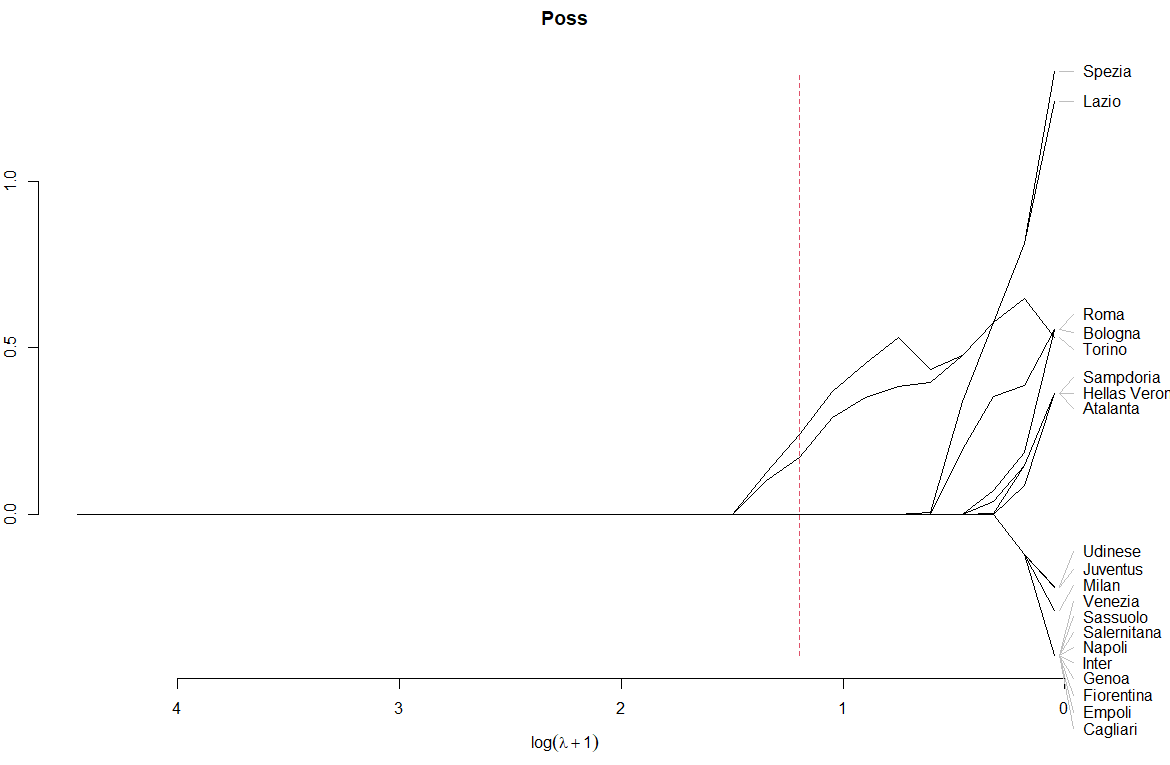
\includegraphics[height=8cm, width=15cm]{possL.png}
		\caption{Grafico che riporta l'andamento della stima del possesso della palla per ogni squadra al variare del parametro di tuning $\lambda$} \label{fig:possL}
	\end{center}
\end{figure}

In Figura \ref{fig:possL} viene mostrato l'andamento relativo alla stima della covariata del possesso della palla, in cui si notano la Lazio e il Torino che si discostano nettamente dall'andamento nullo tenuto dalla maggior parte delle squadre.

\begin{figure}[htbp]
	\begin{center}
		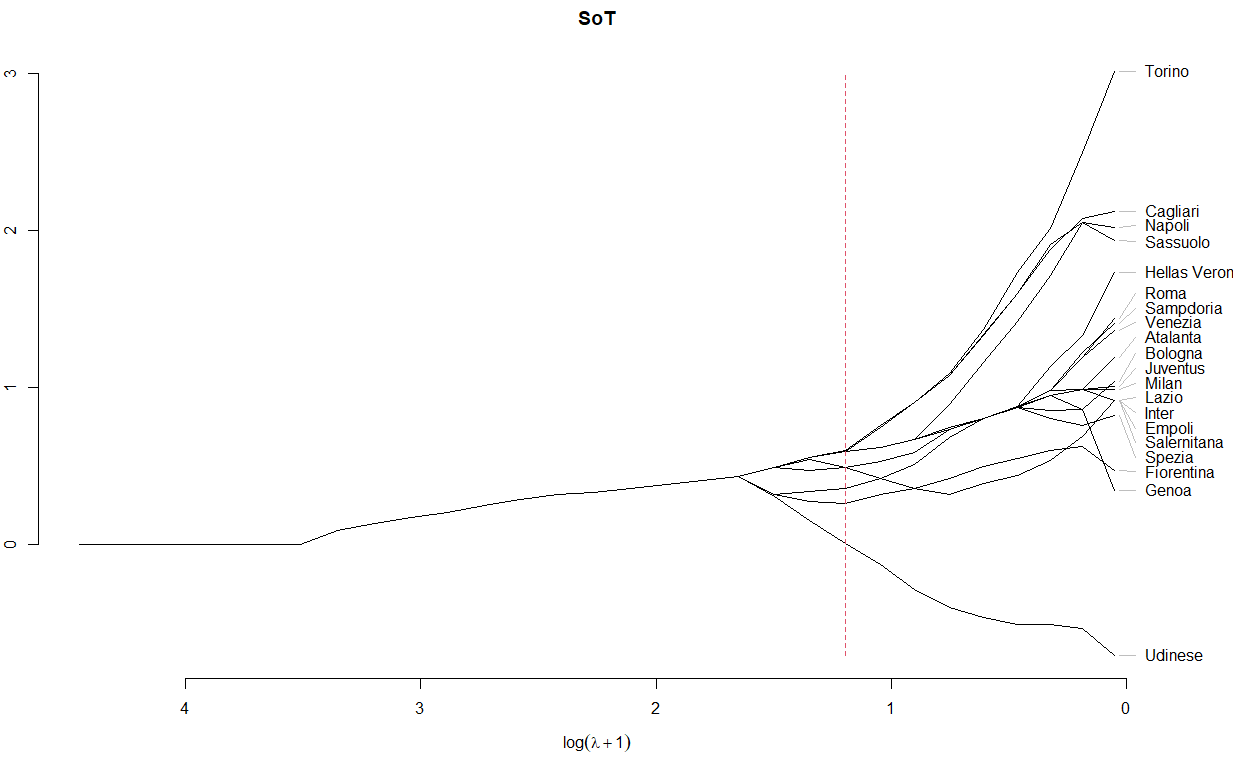
\includegraphics[height=8cm, width=15cm]{sotL.png}
		\caption{Grafico che riporta l'andamento della stima del numero di tiri in porta per ogni squadra al variare del parametro di tuning $\lambda$} \label{fig:sotL}
	\end{center}
\end{figure}

In Figura \ref{fig:sotL} viene mostrato l'andamento relativo alla stima della covariata del numero di tiri in porta. Si notano cinque clusters con stima positiva. Abbiamo il cluster con la stima più alta che contiene la maggioranza delle squadre, seguito dal secondo cluster per stima contenente Inter e Roma. Il terzo cluster per stima contiene solo il Bologna, anche il quarto cluster per stima contiene solo una squadra cioè la Fiorentina. Infine il quinto cluster per stima contiene l'Udinese che ha un valore quasi nullo ma comunque positivo.

\begin{figure}[htbp]
	\begin{center}
		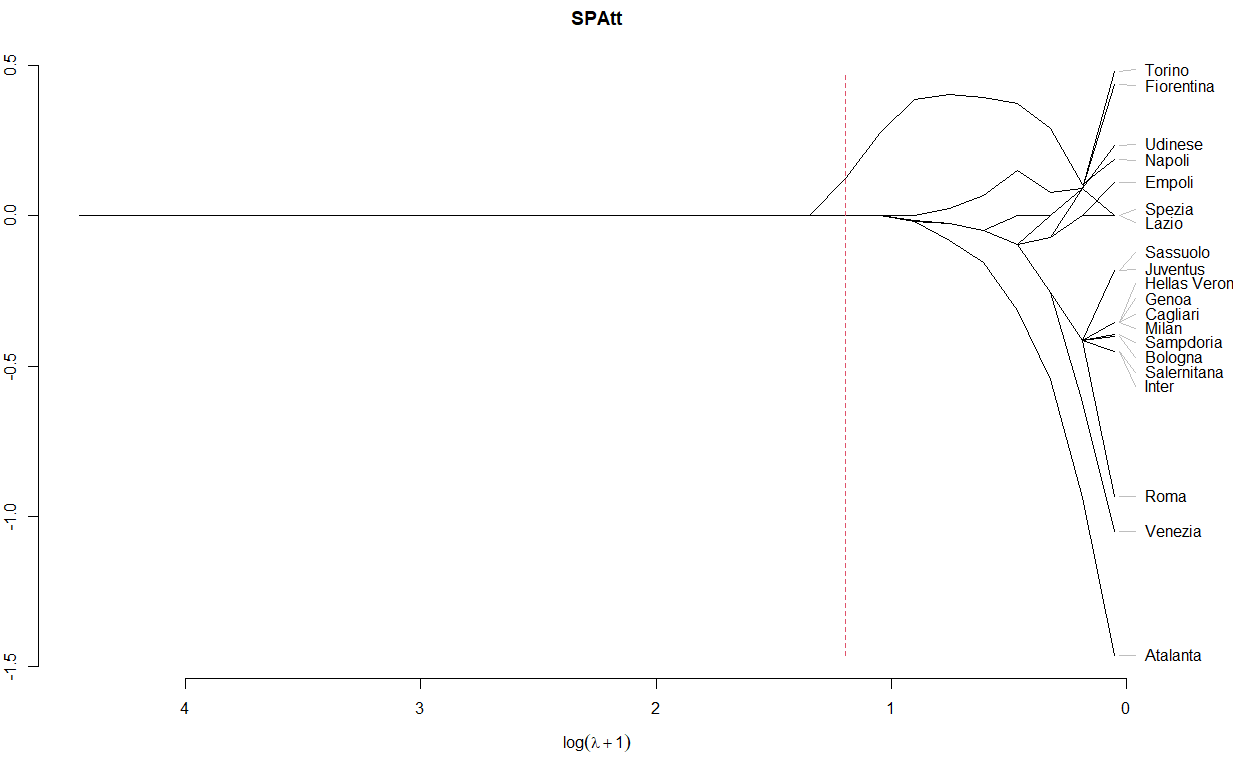
\includegraphics[height=8cm, width=15cm]{spattL.png}
		\caption{Grafico che riporta l'andamento della stima del numero di passaggi corti tentati per ogni squadra al variare del parametro di tuning $\lambda$} \label{fig:spattL}
	\end{center}
\end{figure}

In Figura \ref{fig:spattL} viene mostrato l'andamento relativo alla stima della covariata del numero di passaggi corti tentati. Si nota che il Napoli ha un andamento positivo che si discosta nettamente dall'andamento nullo tenuto dalla maggior parte delle squadre.

\begin{figure}[htbp]
	\begin{center}
		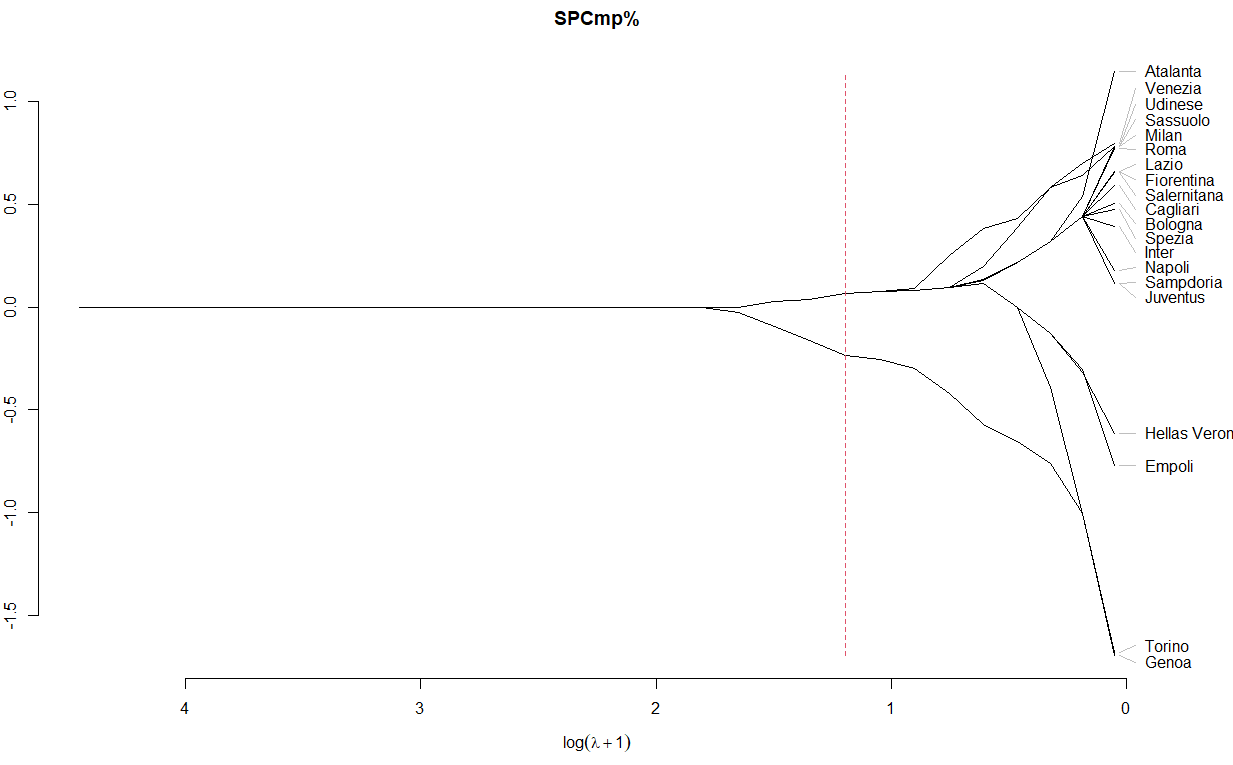
\includegraphics[height=8cm, width=15cm]{spcmpL.png}
		\caption{Grafico che riporta l'andamento della stima della percentuale di passaggi corti riusciti per ogni squadra al variare del parametro di tuning $\lambda$} \label{fig:spcmpL}
	\end{center}
\end{figure}

In Figura \ref{fig:spcmpL} viene mostrato l'andamento relativo alla stima della covariata della percentuale di passaggi corti riusciti. Si nota che il Genoa ha un andamento negativo che si discosta nettamente dall'andamento leggermente positivo tenuto dalla maggior parte delle squadre.

\begin{figure}[htbp]
	\begin{center}
		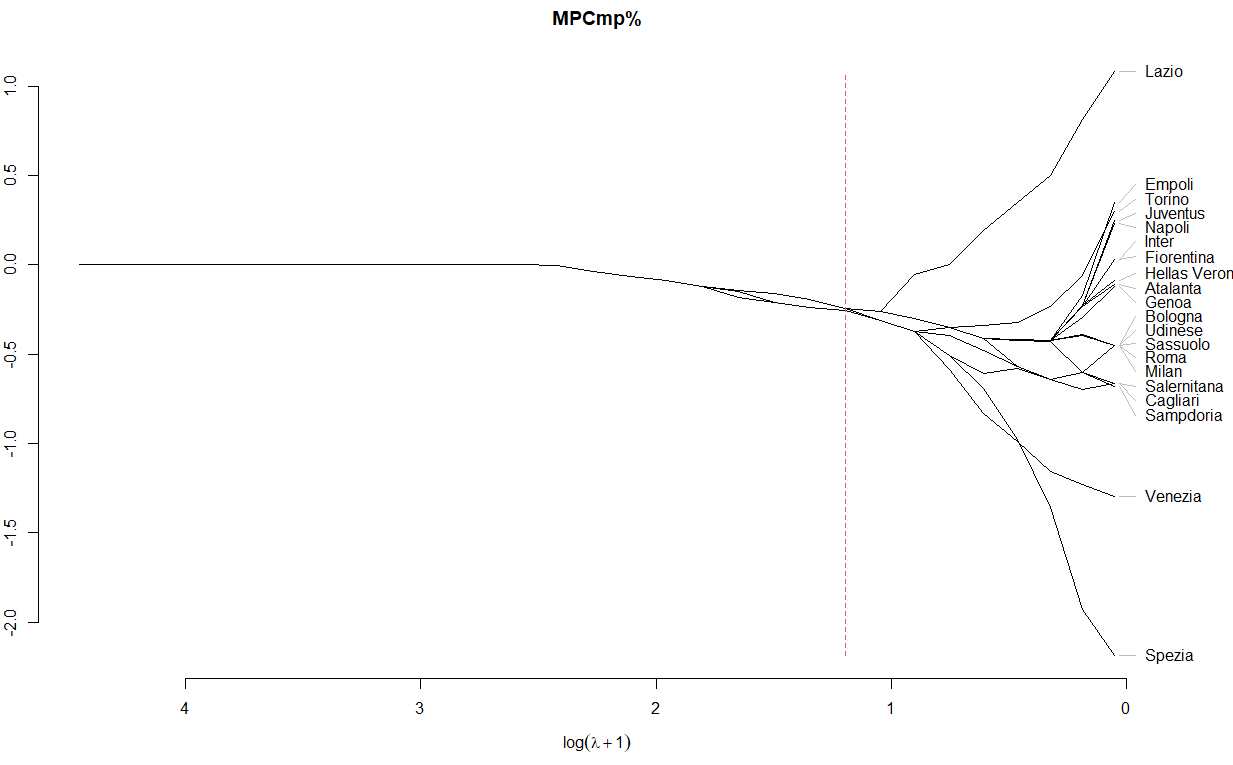
\includegraphics[height=8cm, width=15cm]{mpcmpL.png}
		\caption{Grafico che riporta l'andamento della stima della percentuale di passaggi medi riusciti per ogni squadra al variare del parametro di tuning $\lambda$} \label{fig:mpcmpL}
	\end{center}
\end{figure}

In Figura \ref{fig:mpcmpL} viene mostrato l'andamento relativo alla stima della covariata della percentuale di passaggi medi riusciti. Si nota che il Genoa e il Bologna hanno un andamento leggermente più negativo rispetto all'andamento comunque negativo tenuto dalla maggior parte delle squadre.

\begin{figure}[htbp]
	\begin{center}
		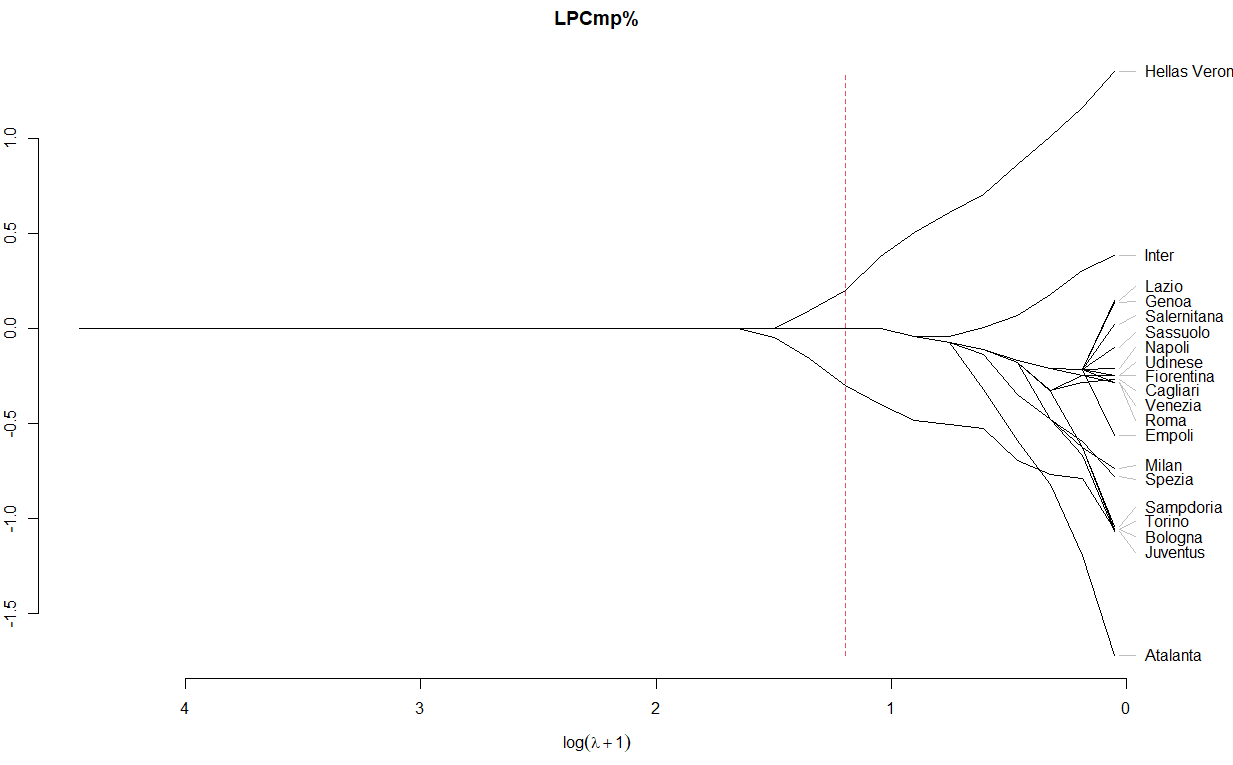
\includegraphics[height=8cm, width=15cm]{lpcmpL.png}
		\caption{Grafico che riporta l'andamento della stima della percentuale di passaggi lunghi riusciti per ogni squadra al variare del parametro di tuning $\lambda$} \label{fig:lpcmpL}
	\end{center}
\end{figure}

In Figura \ref{fig:lpcmpL} viene mostrato l'andamento relativo alla stima della covariata della percentuale di passaggi lunghi riusciti. Ci sono tre clusters. C'è il cluster contenete l'Hellas Verona che ha un percorso positivo, il cluster più grande che contiene quasi tutte le squadre ha un andamento nullo e Infine, il terzo cluster contenete il Bologna ha un andamento negativo.

\begin{figure}[htbp]
	\begin{center}
		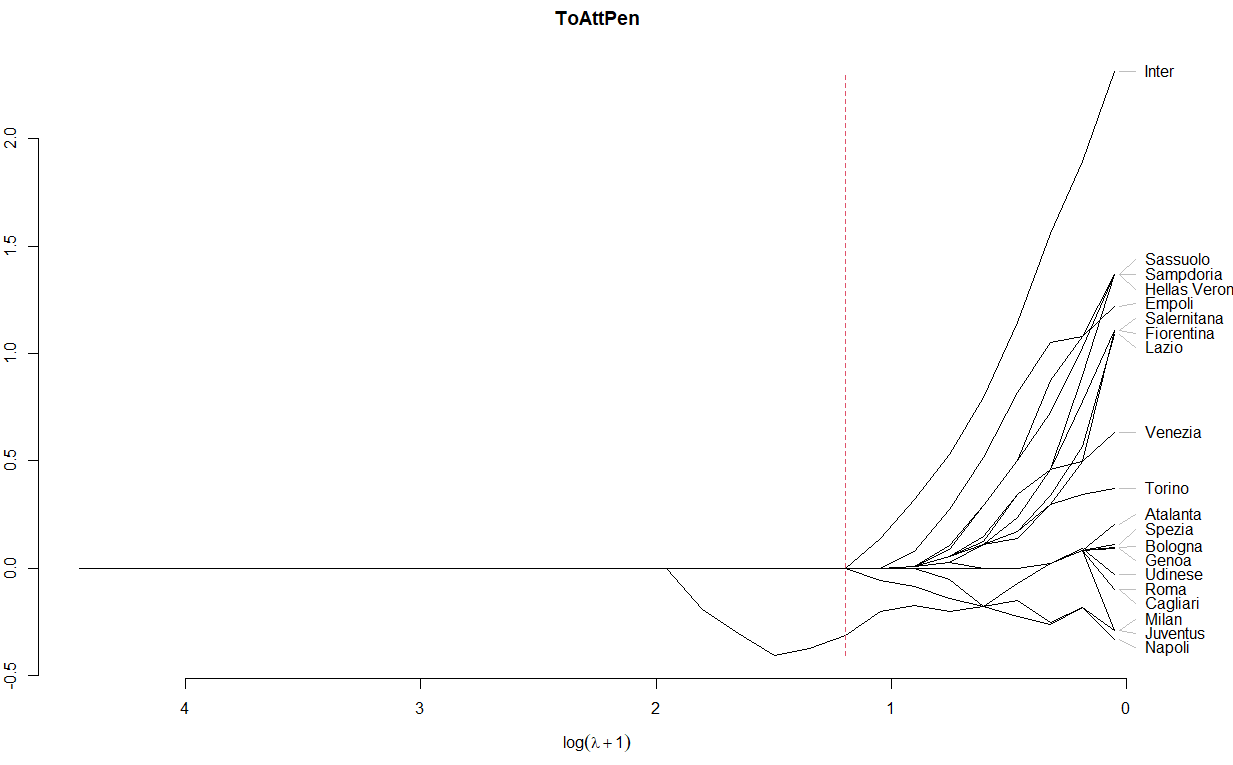
\includegraphics[height=8cm, width=15cm]{toattpenL.png}
		\caption{Grafico che riporta l'andamento della stima del numero di tocchi fatti nell'area di rigore avversaria per ogni squadra al variare del parametro di tuning $\lambda$} \label{fig:toattpenL}
	\end{center}
\end{figure}

In Figura \ref{fig:toattpenL} viene mostrato l'andamento relativo alla stima della covariata del numero di tocchi fatti nell'area di rigore avversari. Si nota che l'Atalanta ha un andamento negativo che si discosta nettamente dall'andamento nullo tenuto dalla maggior parte delle squadre.

\begin{figure}[htbp]
	\begin{center}
		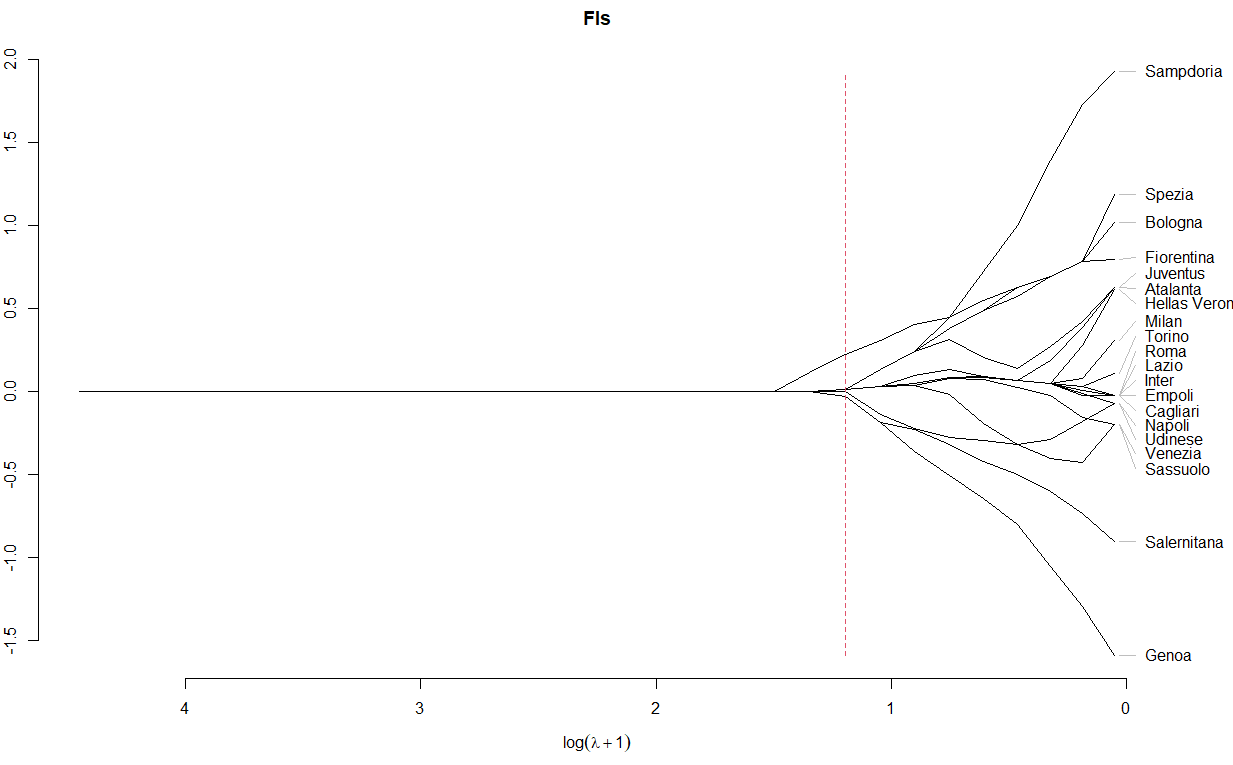
\includegraphics[height=8cm, width=15cm]{flsL.png}
		\caption{Grafico che riporta l'andamento della stima del numero di falli subiti per ogni squadra al variare del parametro di tuning $\lambda$} \label{fig:flsL}
	\end{center}
\end{figure}

In Figura \ref{fig:flsL} viene mostrato l'andamento relativo alla stima della covariata del numero di falli subiti, in cui si notano quattro clusters. C'è il cluster contenete il Bologna che ha un percorso positivo, il cluster più grande che contiene quasi tutte le squadre che ha un andamento leggermente positivo. Invece il cluster che contiene il Napoli ha un andamento leggermente negativo, mentre ancora più negativo è il cluster contente il Genoa e la Salernitana.

\begin{figure}[htbp]
	\begin{center}
		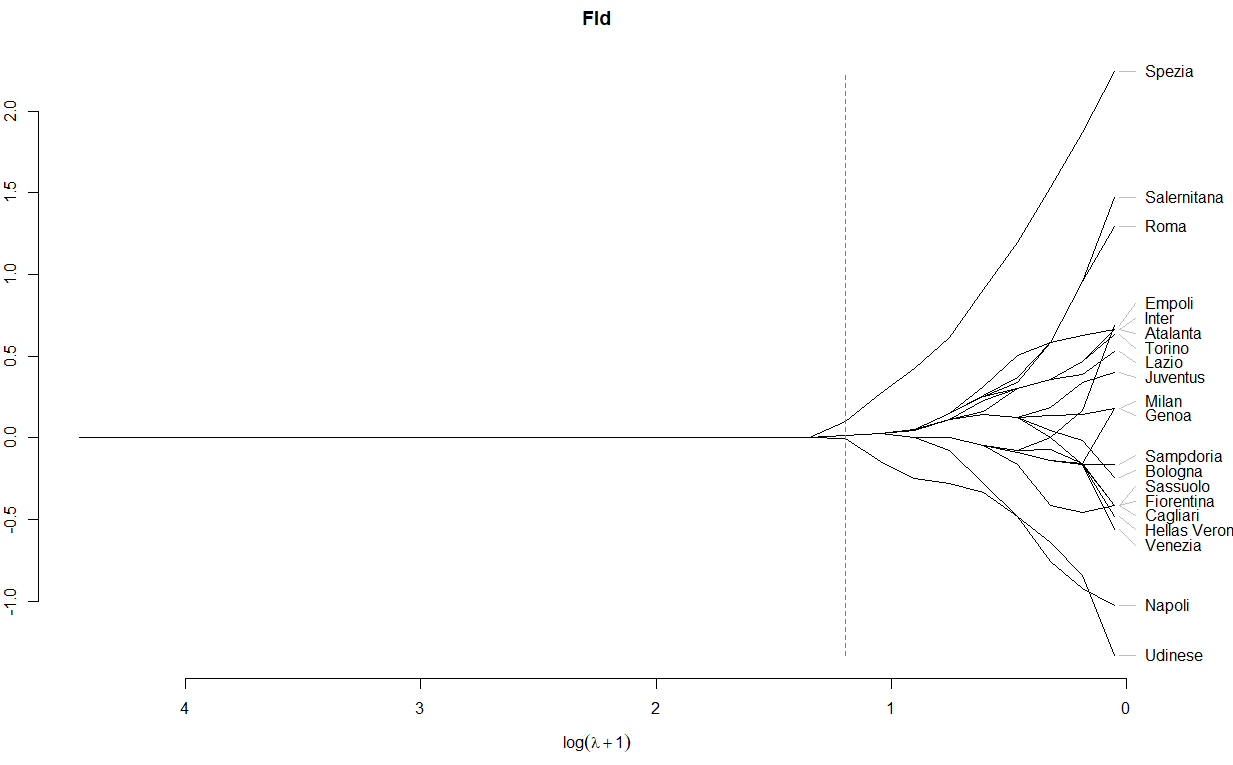
\includegraphics[height=8cm, width=15cm]{fldL.png}
		\caption{Grafico che riporta l'andamento della stima del numero di falli fatti per ogni squadra al variare del parametro di tuning $\lambda$} \label{fig:fldL}
	\end{center}
\end{figure}

In Figura \ref{fig:fldL} viene mostrato l'andamento relativo alla stima della covariata del numero di falli fatti, in cui si notano tre clusters. C'è il cluster contenete lo Spezia che ha un percorso positivo, il cluster più grande che contiene quasi tutte le squadre che ha un andamento leggermente positivo. Invece il cluster che contiene l'Udinese ha un andamento leggermente negativo.

\begin{figure}[htbp]
	\begin{center}
		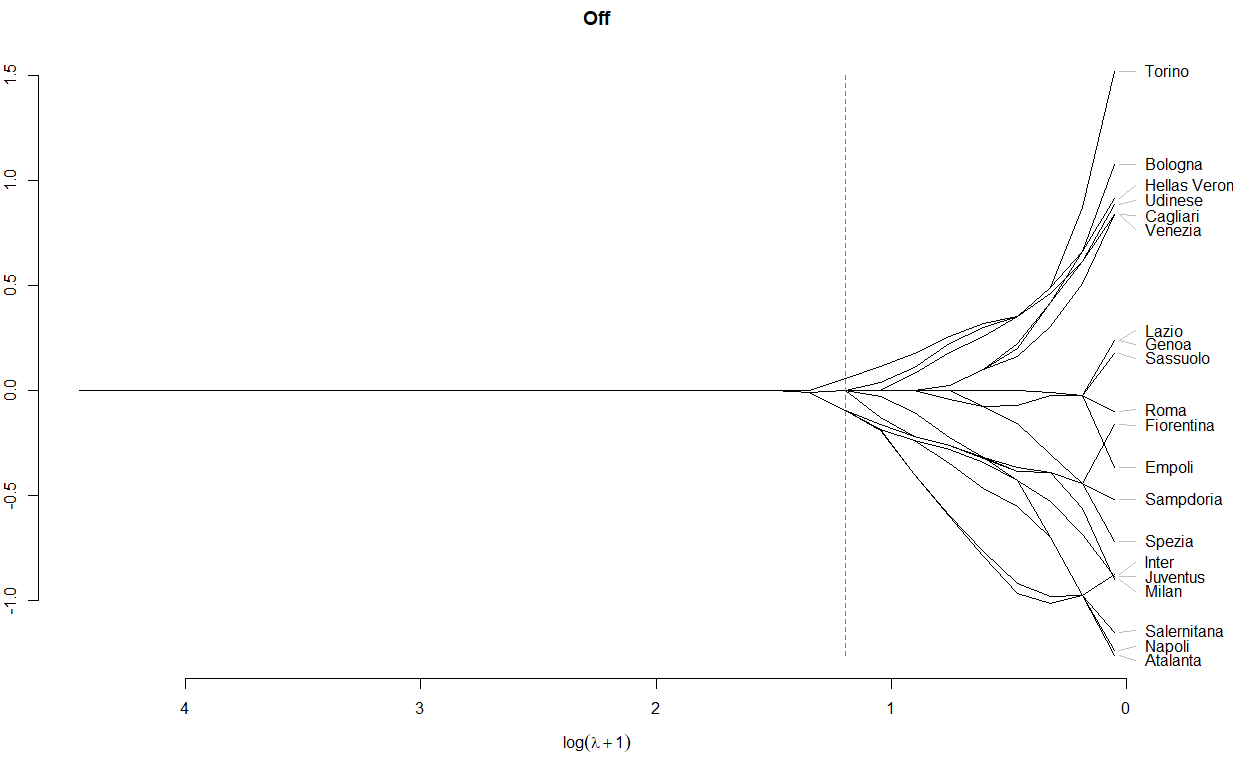
\includegraphics[height=8cm, width=15cm]{offL.png}
		\caption{Grafico che riporta l'andamento della stima del numero di fuorigioco fatti per ogni squadra al variare del parametro di tuning $\lambda$} \label{fig:offL}
	\end{center}
\end{figure}

In Figura \ref{fig:offL} viene mostrato l'andamento relativo alla stima della covariata del numero di fuorigioco fatti. Ci sono tre clusters. C'è il cluster contenete l'Hellas Verona che ha un percorso positivo, il cluster più grande che contiene quasi tutte le squadre che ha un andamento leggermente positivo. Infine c'è il cluster che contiene il Milan, l'Inter, il Napoli e la Juventus che ha un andamento negativo.

\begin{figure}[htbp]
	\begin{center}
		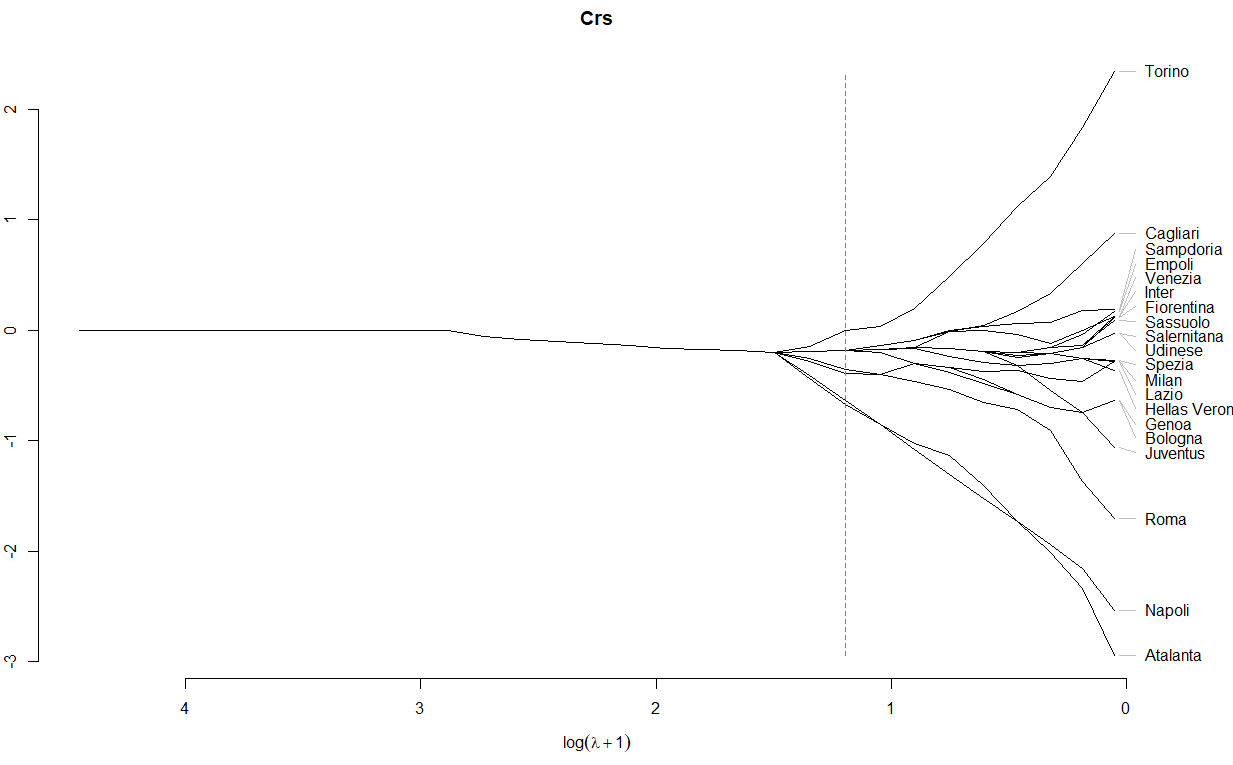
\includegraphics[height=8cm, width=15cm]{crsL.png}
		\caption{Grafico che riporta l'andamento della stima del numero di cross fatti per ogni squadra al variare del parametro di tuning $\lambda$} \label{fig:crsL}
	\end{center}
\end{figure}

In Figura \ref{fig:crsL} viene mostrato l'andamento relativo alla stima della covariata del numero di cross fatti. Ci sono quattro clusters. C'è il cluster contenete il Torino che ha un andamento nullo, il cluster più grande che contiene quasi tutte le squadre che ha un percorso negativo. Ancora più negativi sono i percorsi del cluster contenente il Milan e la Roma, secondo solo al cluster contenente l'Atalanta e il Napoli che si discosta nettamente da tutti gli altri clusters.

\begin{figure}[htbp]
	\begin{center}
		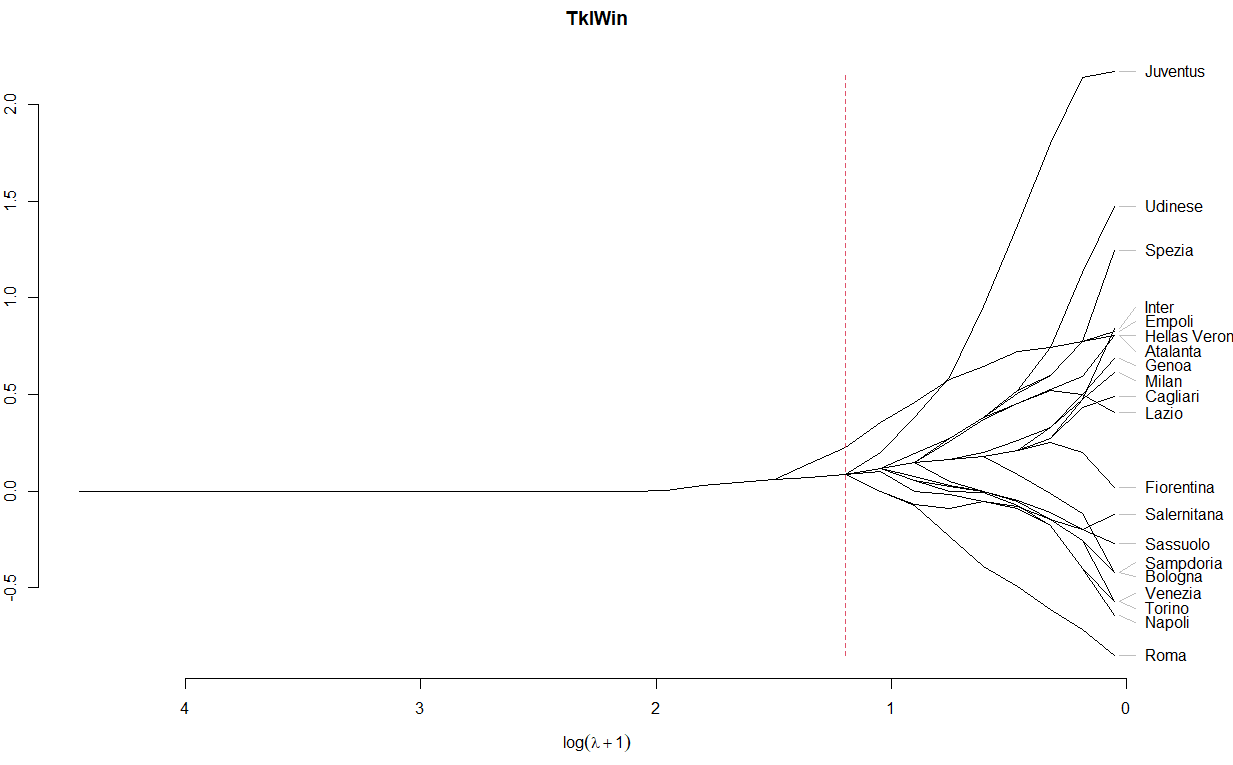
\includegraphics[height=8cm, width=15cm]{tklwinL.png}
		\caption{Grafico che riporta l'andamento della stima del numero di contrasti vinti per ogni squadra al variare del parametro di tuning $\lambda$} \label{fig:tklwinL}
	\end{center}
\end{figure}

\begin{figure}[htbp]
	\begin{center}
		\includegraphics[height=8cm, width=15cm]{recovL.png}
		\caption{Grafico che riporta l'andamento della stima del numero di recuperi per ogni squadra al variare del parametro di tuning $\lambda$} \label{fig:recovL}
	\end{center}
\end{figure}
In Figura \ref{fig:tklwinL} viene mostrato l'andamento relativo alla stima della covariata del numero di contrasti vinti, in cui si nota che l'Empoli ha un percorso positivo che si discosta nettamente dall'andamento comunque positivo ma in minor misura, tenuto dalla maggior parte delle squadre.\\
In Figura \ref{fig:recovL} viene mostrato l'andamento relativo alla stima della covariata del numero di recuperi. Si nota che l'Udinese ha un percorso leggermente più negativo rispetto all'andamento negativo tenuto dalla maggior parte delle squadre.\\

Per riassumere quanto visto fin ora, la Figura \ref{fig:l2BTCL} mostra i percorsi delle norme L2 che rappresentano l'importanza complessiva dei singoli effetti delle covariate.

\begin{figure}[htbp]
	\begin{center}
		\includegraphics[height=8cm, width=15cm]{L2.png}
		\caption{Grafico che riporta l'importanza delle covariate rispetto alle norme L2 al variare del parametro di tuning $\lambda$} \label{fig:l2BTCL}
	\end{center}
\end{figure}
Dal grafico si nota che il rapporto tiri-gol \texttt{G/Sh} è la variabile che incide maggiormente nella determinazione dell'esito di una partita. Analogamente anche il numero di tiri in porta \texttt{SoT} e il numero di parate \texttt{Saves} sono determinanti dell'esito di una partita, ma con un minor peso rispetto a \texttt{G/Sh}. Anche il numero di cross \texttt{Crs} determina in modo significativo l'esito della partita, ma al contrario di \texttt{G/Sh} sappiamo che contribuisce a diminuire le probabilità di vittoria. Si nota anche qui che il possesso della palla ha un ruolo molto marginale nel determinare il risultato di una partita. Viene confermata la tendenza che mantenere il pallone in zone difensive con meno transizioni in zone d'attacco sembra che dia maggior probabilità di vittoria. Si riconferma il numero di lanci lunghi tentati \texttt{LPAtt} importante per l'esito della partita e che favorisce la vittoria. Al contrario le altre variabili esplicative legate ai passaggi che sono poco determinanti e diminuiscono la probabilità di vittoria. Dal grafico si nota che sia il numero di contrasti vinti \texttt{TklWin} e il numero di fuorigioco \texttt{Off} sono determinanti, diversamente il numero di recuperi \texttt{Recov}, la distanza percorsa con la palla \texttt{TotDist} e il numero di intercetti \texttt{Int} sono poco significativi. Infine notiamo che il numero di falli fatti \texttt{fld} è più determinante di quelli subiti \texttt{fls}.\\
Perciò, la maggior parte delle stime ottenute sembrano essere in linea con i risultati osservati nel precedente modello con covariate specifiche dell'oggetto senza l'applicazione del metodo \emph{LASSO}.

\section{BTM senza l'intercetta e con LASSO}
Come era stato accennato nel Capitolo \ref{cap:BT} l'intercetta spiega la maggior parte dell'abilità relativa alla squadra. Per cui le covariate possono essere viste come estensioni contenenti effetti aggiuntivi dell'abilità della squadra che non sono spiegati dall'intercetta. In tal senso, gli effetti della covariata possono aiutare a spiegare i risultati imprevisti di un partita che non possono essere completamente spiegati esclusivamente dall'intercetta. Nelle tre precedenti applicazione del modello Bradley-Terry si è sempre inserita un intercetta per ogni squadra, anche nel modello \hyperref[for:3.9]{(4.9)}. Perciò, di seguito verranno mostrati i risultati relativi a un modello Bradley-Terry della stessa forma del modello \hyperref[for:4.9]{(4.12)} ma senza le intercette, con lo scopo di capire qual'è l'effetto totale che ha ogni variabile esplicativa sull'abilità della squadra senza l'interferenza dell'intercetta che copre l'effetto della covariata. Ovviamente dato il numero elevato di covariate è stata applicata una selezione attraverso il metodo \emph{LASSO}. Il modello applicato è il seguente
\begin{align}
	P(Y_{p(i,j)}\leq k) =  \frac{exp(\delta_i + \theta_{k} + x^T_{pi}\eta_i - x^T_{pj}\eta_j)}{1 + exp(\delta_i + \theta_{k} + x^T_{pi}\eta_i - x^T_{pj}\eta_j)},\label{for:5.2}
\end{align}

Nella Tabella \ref{tab:BTCLI2} e nella Tabella \ref{tab:BTCLI3} vengono riportati i risultati nella stessa modalità utilizza nella precedente sezione.
\begin{table}[]%
	
	\renewcommand{\arraystretch}{1.7}
	\centering
	\begin{tabular}{ccp{10cm}}
		\hline	
		
		\textbf{Covariata} & \textbf{Stima} & \textbf{Squadra} \\	
		\hline
		Home & 0.270 & Tutti\\
		Poss & 0.299 & Lazio \\
		Poss & 0.047 & Tutti tranne Lazio\\
		Sh & 0.317 & Tutti \\
		SoT & 0.495 & Atalanta, Cagliari, Empoli, Genoa, Verona, Juventus, Lazio, Milan, Napoli, Roma, Salernitana, Sampdoria, Sassuolo, Spezia, Torino e Venezia\\
		SoT & 0.438 & Inter\\
		SoT & 0.399 & Bologna, Fiorentina e Udinese \\
		G/Sh & 0.867 & Tutti \\
		Saves & 0.242 & Tutti \\
		PAtt & 0.000 & Tutti \\
		PCmp\% & 0.000 & Tutti \\
		SPAtt & 0.000 & Tutti \\
		SPCmp\% & 0.000 & Tutti tranne Genoa \\ 
		SPCmp\% & -0.076 & Genoa \\	
		MPAtt & 0.000 & Tutti \\ 
		MPCmp\% & -0.230 & Udinese \\
		MPCmp\% & -0.236 & Tutti tranne Udinese \\		
		LPAtt & 0.178 & Tutti \\
		LPCmp\% & 0.016 & Hellas Verona \\
		LPCmp\% & 0.000 & Tutti tranne Verona \\
		ToDefPen & 0.080 & Tutti \\      
		ToDef3rd & 0.024 & Tutti \\
		
		
		\hline
		& &  \\
		
	\end{tabular} \hbox{}
	\caption{Stime delle covariate.} \label{tab:BTCLI2} 
	
\end{table}

\begin{table}[]%
	
	\renewcommand{\arraystretch}{1.7}
	\centering
	\begin{tabular}{ccp{10cm}}
		\hline	
		
		\textbf{Covariata} & \textbf{Stima} & \textbf{Squadra} \\	
		\hline
		ToMid3rd & 0.002 & Tutti tranne Inter e Sampdoria\\
		ToMid3rd & 0.000 & Inter e Sampdoria\\
		ToAtt3rd & -0.013 & Tutti \\  
		ToAttPen & 0.035 & Tutti tranne Atalanta \\    
		ToAttPen & -0.083 & Atalanta \\ 	     	 
		TotDist & 0.000 & Tutti \\	
		Fls & 0.256 & Bologna  \\
		Fls & 0.088 & Tutti tranne Bologna \\ 		
		Fld & 0.066 & Tutti tranne Udinese \\
		Fld & 0.023 & Udinese \\
		Off & 0.055 & Hellas Verona\\
		Off & 0.000 & Tutti tranne Juventus\\
		Off & -0.085 & Juventus  \\
		Crs & -0.190 & Tutti tranne Atalanta\\
		Crs & -0.464 & Atalanta \\
		Int & 0.000 & Tutti\\
		TklWin &  0.117 & Empoli  \\
		TklWin &  0.000 & Tutti tranne Empoli  \\ 
		Recov &  0.000 & Tutti \\ 
		\hline
		& &  \\
		
	\end{tabular} \hbox{}
	\caption{Stime delle covariate.} \label{tab:BTCLI3} 
	
\end{table}
Anche in questa applicazione sono state eliminate alcune covariate. Come già visto nel modello precedente, vengono confermate l'eliminazione del numero di passaggi tentati \texttt{PAtt}, della percentuale dei passaggi completati \texttt{PCmp\%} e della distanza percorsa con la palla \texttt{TotDist}. Viene tolta dal modello la variabile esplicativa del numero di passaggi corti tentati \texttt{SPAtt} che nel modello precedente andava a aumentare le probabilità di vittoria solo per il Napoli. Viene eliminata la covariata del numero di passaggi medi tentati \texttt{MPAtt} e quella del numero di intercettazioni \texttt{Int}. Infine abbiamo l'eliminazione della variabile esplicativa che indica il numero di recuperi che nel precedente modello era valutata come una covariata che incideva negativamente sulla probabilità di vittoria.\\

In questa nuovo tipo di modello la stima del parametro del possesso palla \texttt{Poss} ha subito un piccola variazione. Infatti ora la stima non è più nulla per la maggior parte delle squadre ma e leggermente positiva. Ciononostante la significatività si riconferma ancora bassa. Si riconferma però significativa solo per il gioco della Lazio ma non più per il Torino come nello scorso modello. Tale risultato è visibili nella Figura \ref{fig:possLI}.\\
\begin{figure}[]
	\begin{center}
		\includegraphics[height=8cm, width=15cm]{possLI.png}
		\caption{Grafico che riporta l'andamento della stima del possesso della palla per ogni squadra al variare del parametro di tuning $\lambda$} \label{fig:possLI}
	\end{center}
\end{figure}
Il numero di tiri \texttt{Sh}, il rapporto tiri-gol \texttt{G/Sh} e il numero di parate \texttt{Saves} sono ancora determinati per aumentare la probabilità di vittoria. Analogamente anche il numero di tiri in porta \texttt{SoT} mantiene sia una stima positiva del parametro, e sia la sua variabilità seppur più ristretta rispetto al modello precedente. Infatti nella Figura \ref{fig:sotLI} è possibile individuare tre clusters. Il più grande con la maggiore stima contiene la maggior parte delle squadre. Il secondo contiene solo l'Inter e infine il terzo contiene le squadre: Bologna, Fiorentina e Udinese. Il risultato è visibile nella Figura \ref{fig:sotLI} \\
\begin{figure}[htbp]
	\begin{center}
		\includegraphics[height=8cm, width=15cm]{sotLI.png}
		\caption{Grafico che riporta l'andamento della stima del numero di tiri in porta per ogni squadra al variare del parametro di tuning $\lambda$} \label{fig:sotLI}
	\end{center}
\end{figure}
Nella percentuale di passaggi corti riusciti \texttt{SPCmp\%} ora viene a crearsi un cluster con un percorso nullo contenente quasi tutte le squadre eccetto il Genoa che è contenuto in un cluster con un percorso negativo. Tali risultati sono visibili nella Figura \ref{fig:spcmpLI}.\\
\begin{figure}[htbp]
	\begin{center}
		\includegraphics[height=8cm, width=15cm]{spcmpLI.png}
		\caption{Grafico che riporta l'andamento della stima della percentuale di passaggi corti riusciti per ogni squadra al variare del parametro di tuning $\lambda$} \label{fig:spcmpLI}
	\end{center}
\end{figure}
Per la variabile esplicativa della percentuale di passaggi medi riusciti \texttt{MPCmp\%} ora viene a crearsi un cluster con un percorso fortemente negativo contenente quasi tutte le squadre eccetto l'Udinese dove si distingue per avere un percorso leggermente meno negativo. Tali risultati sono visibili nella Figura \ref{fig:mpcmpLI}.\\
\begin{figure}[]
	\begin{center}
		\includegraphics[height=8cm, width=15cm]{mpcmpLI.png}
		\caption{Grafico che riporta l'andamento della stima della percentuale di passaggi medi riusciti per ogni squadra al variare del parametro di tuning $\lambda$} \label{fig:mpcmpLI}
	\end{center}
\end{figure}
Il numero di passaggi lunghi tentati è ancora una covariata con una stima del parametro che aumenta la probabilità di vittoria. Si nota che la stima della covariata della percentuale di passaggi lunghi riusciti \texttt{LPCmp\%} ha un cluster con un percorso nullo contenente quasi tutte le squadre eccetto l'Hellas Verona che si distingue con un percorso positivo. Tali risultati sono visibili nella Figura \ref{fig:lpcmpLI}.\\
\begin{figure}[htbp]
	\begin{center}
		\includegraphics[height=8cm, width=15cm]{lpcmpLI.png}
		\caption{Grafico che riporta l'andamento della stima della percentuale di passaggi lunghi riusciti per ogni squadra al variare del parametro di tuning $\lambda$} \label{fig:lpcmpLI}
	\end{center}
\end{figure}
Sia il numero di tocchi fatti in area di rigore \texttt{ToDefPen} e sia il numero di tocchi fatti nella trequarti di difesa \texttt{ToDef3rd} aumentano la probabilità di vittoria. Nella stima del parametro della covariata che indica il numero di tocchi fatti a centrocampo \texttt{ToMid3rd}, viene a crearsi un cluster con un percorso quasi nullo contenente quasi tutte le squadre eccetto l'Inter e la Sampdoria, le quali formano un cluster con un percorso nullo.\\
Il numero di tocchi fatti nella trequarti offensiva \texttt{ToAtt3rd} è ancora stimato con un peso che diminuisce la probabilità di vittoria.\\
Per la stima della variabile esplicativa che indica il numero di tocchi fatti nell'area di rigore avversaria \texttt{ToAttPen}, c'è un cluster con un percorso negativo contenente quasi tutte le squadre eccetto l'Atalanta che si distingue con un percorso positivo. Tali risultati sono visibili nella Figura \ref{fig:toattpenLI}.\\
\begin{figure}[htbp]
	\begin{center}
		\includegraphics[height=8cm, width=15cm]{toattpenLI.png}
		\caption{Grafico che riporta l'andamento della stima del numero di tocchi fatti nell'area di rigore avversaria per ogni squadra al variare del parametro di tuning $\lambda$} \label{fig:toattpenLI}
	\end{center}
\end{figure}
Per quanto riguarda l'aggressività della squadra il numero di falli fatti \texttt{Fld} aumenta la probabilità di vittoria per tutte le squadre. Come mostrato della Figura \ref{fig:fldLI} però, la stima per l'Udinese è minore rispetto a tutte le altre squadre. Analogamente anche il numero di falli subiti \texttt{Fls} aumenta la probabilità di vittoria di tutte le squadre, in particolare il Bologna si distingue con una stima maggiore come mostrato nella Figura \ref{fig:flsLI}.\\
\begin{figure}[]
	\begin{center}
		\includegraphics[height=8cm, width=15cm]{fldLI.png}
		\caption{Grafico che riporta l'andamento della stima del numero di falli fatti per ogni squadra al variare del parametro di tuning $\lambda$} \label{fig:fldLI}
	\end{center}
\end{figure}
\begin{figure}[htbp]
	\begin{center}
		\includegraphics[height=8cm, width=15cm]{flsLI.png}
		\caption{Grafico che riporta l'andamento della stima del numero di falli subiti per ogni squadra al variare del parametro di tuning $\lambda$} \label{fig:flsLI}
	\end{center}
\end{figure}

Nella stima della covariata che indica il numero di fuorigioco fatti \texttt{Off}, viene a crearsi un cluster con un percorso nullo contenente quasi tutte le squadre eccetto la Juventus, la quale forma un cluster con un percorso negativo, tali risultati sono visibili nella Figura \ref{fig:offLI}.\\
\begin{figure}[htbp]
	\begin{center}
		\includegraphics[height=8cm, width=15cm]{offLI.png}
		\caption{Grafico che riporta l'andamento della stima del numero di fuorigioco fatti per ogni squadra al variare del parametro di tuning $\lambda$} \label{fig:offLI}
	\end{center}
\end{figure}
La stima della variabile esplicativa del numero di cross fatti \texttt{Crs} si conferma essere ancora determinante per diminuire la probabilità di vittoria. L'Atalanta inoltre si distingue dalle altre squadre con un percorso ancora pù negativo rispetto, come mostrato nella Figura \ref{fig:crsLI}.\\
\begin{figure}[htbp]
	\begin{center}
		\includegraphics[height=8cm, width=15cm]{crsLI.png}
		\caption{Grafico che riporta l'andamento della stima del numero di cross fatti per ogni squadra al variare del parametro di tuning $\lambda$} \label{fig:crsLI}
	\end{center}
\end{figure}
Si nota che nella stima della covariata che indica il numero di contrasti vinti \texttt{TklWin}, viene a crearsi un cluster con un percorso nullo contenente quasi tutte le squadre eccetto l'Empoli, il quale forma un cluster con un percorso positivo. Tali risultati sono visibili nella Figura \ref{fig:tklwinLI}.\\
\begin{figure}[htbp]
	\begin{center}
		\includegraphics[height=8cm, width=15cm]{tklwinLI.png}
		\caption{Grafico che riporta l'andamento della stima del numero di contrasti vinti per ogni squadra al variare del parametro di tuning $\lambda$} \label{fig:tklwinLI}
	\end{center}
\end{figure}
Infine, viene confermato che giocare la partita \texttt{Home} ha un effetto positivo stimato in 0.270, mentre è cambiato la stima delle soglie $\theta_1$ e $\theta_2$ che valgono rispettivamente -0.803  e 0.803 .\\
Tutti i risultati sono stati ottenuti impostando come parametro di tuning $lambda$ pari a 3.299.\\

Un ulteriore analisi che può essere condotta, è analizzare l'effetto medio dei valori assunti per ogni partita e per ogni squadra delle covariate, insieme alle stime dei singoli parametri per squadra. Si utilizzeranno i grafici a \emph{effetto stella} proposti da \textcite{tutz2013visualization}. In questi grafici è possibile visualizzare i valori medi per squadra e per covariata moltiplicati per le rispettive stime riportate precedentemente. Quindi verrà illustrato graficamente il contributo medio di una variabile esplicativa sull'abilità di una singola squadra. Il grafico funziona nel seguente modo: esso mostra il prodotto esponenziale tra la media dei valori assunti da una covariate e le sue stime per ogni squadra. Per ogni grafico, viene creato un cerchio con raggio \emph{exp(0) = 1} il quale rappresenta il caso con stima nulla. I valori oltre il cerchio indica che la covariata ha effetto positivo in media sulla squadra, viceversa, i valori all'interno del cerchio indicano che la variabile esplicativa applica effetti negativi in media sulla squadra. Nella Figura \ref{fig:effstar1} nella Figura \ref{fig:effstar2} e nella Figura \ref{fig:effstar3} vengono mostrati i grafici a \emph{effetto stella}.
Nella Figura \ref{fig:effstar1} si possono vedere tutte le variabili esplicative con una stima nulla ma anche quelle covariate dove c'erano alcune squadre che si differenziavano dalle altre con una stima differente da quella nulla. Ad esempio la Lazio con il possesso palla \texttt{Poss} e l'Empoli con il numero di contrasti vinti \texttt{TklWin}.\\

\begin{figure}[htbp]
	\begin{center}
		\includegraphics[height=9cm, width=15cm]{effstar.png}
		\caption{Grafico che riporta il contributo medio di una covariata sull'abilità di una singola squadra secondo il modello \ref{for:5.2}.} \label{fig:effstar1}
	\end{center}
\end{figure}

Per la Figura \ref{fig:effstar2} abbiamo due particolari grafici. Entrambi rappresentano l'effetto negativo delle covariate che indicano rispettivamente, il numero di tocchi nella trequarti avversaria fatti \texttt{ToAtt3rd} e il numero di cross fatti \texttt{Crs}. In particolare notiamo che a subire più gli effetti negativi sono l'Inter e l'Atalanta in entrambe le variabili esplicative. 


\begin{figure}[htbp]
	\begin{center}
		\includegraphics[scale = 0.40]{estarL2.png}
		\caption{Grafico che riporta il contributo medio di una covariata sull'abilità di una singola squadra secondo il modello \ref{for:5.2}.} \label{fig:effstar2}
	\end{center}
\end{figure}

Infine, risultati più interessanti si hanno nella Figura \ref{fig:effstar3}. Innanzitutto si vede che nella nel grafico del numero di tiri \texttt{Sh} l'Inter ha un grosso beneficio, ma anche in minor misura il Milan, la Roma, l'Atalanta, il Napoli, la Juventus e il Sassuolo. Perciò in generale come già visto \texttt{Sh} ha un effetto positivo e ancora di più per le squadre elencate. Analoghi risultati sono visibili con il numero di tiri in porta \texttt{SoT} con l'aggiunta della Lazio tra le squadre che ricevano più benefici. In generale, nel grafico del numero di parate \texttt{Saves} tutte le squadre ottengo benefici, stesso risultato ma più importante anche con il numero di passaggi lunghi tentati \texttt{LPAtt}. Nel grafico del numero di tocchi in area di rigore \texttt{ToDefPen} c'è un particolare beneficio ottenuto dal Venezia ma anche dell'Inter, dalla Lazio, dall'Empoli e dal Sassuolo. Analoghi risultati anche per il numero di tocchi nella trequarti difensiva \texttt{ToDef3rd}, ma con la differenza di minori benefici per il Venezia. Pertanto, si nota la tendenza delle squadre italiana a attuare tattiche che prediligono di giocare nella propria metà campo. Il numero di tocchi a centrocampo \texttt{ToMid3rd} vengono in media effettuati molto dalle squadre, tranne per le eccezioni Inter e Sampdoria dove l'effetto è nullo. Analogo effetto anche per il numero di tocchi fatti in area di rigore \texttt{ToAttPen}, con l'unica differenza che ora Inter e Sampdoria hanno un effetto positivo e solo l'Atalanta ha un effetto negativo. In generali i falli subiti \texttt{Fls} portano benefici alle squadre sopratutto al Bologna come si era notato dalle stime del modello. Per i falli fatti invece abbiamo che l'Udinese ha minor benefici rispetto a tutte le altri squadre come visto nelle stime.\\
\begin{figure}[htbp]
	\begin{center}
		\includegraphics[height=16cm, width=16cm]{estarL.png}
		\caption{Grafico che riporta il contributo medio di una covariata sull'abilità di una singola squadra secondo il modello \ref{for:5.2}.} \label{fig:effstar3}
	\end{center}
\end{figure}

Infine come fatto nella sezione precedente, si analizzano i percorsi delle norme L2 che rappresentano l'importanza complessiva dei singoli effetti delle covariate. Tali percorsi sono visibili nella Figura \ref{fig:IL2}.

\begin{figure}[htbp]
	\begin{center}
		\includegraphics[height=8cm, width=15cm]{IL2.png}
		\caption{Grafico che riporta l'importanza delle covariate rispetto alle norme L2 al variare del parametro di tuning $\lambda$} \label{fig:IL2}
	\end{center}
\end{figure}

Gli andamenti ottenuti nella Figura \ref{fig:IL2} sono molto simili a quelli visti nella Figura \ref{fig:l2BTCL}, con però un aumento di importanza per la covariata \texttt{ToAttPen} in termini di diminuzione della probabilità di vittoria. Pertanto, quanto ricavato del modello (\ref{for:4.9}) ora trova conferma anche nel modello (\ref{for:5.2}).\\

\section{Conclusione dei risultati ottenuti}(BOZZA)
(*****Probabilmente da spostare nel capitolo delle conclusioni*****)\\

Dai risultati ottenuti e dalle analisi condotte è possibile affermare la seguente conclusione. Nel campionato italiano per poter vincere o comunque ottenere dei buoni risultati la squadra deve adottare un comportamento tattico e giocare prevalentemente nella propria metà campo. Quindi, un comportamento meno propenso a controllare il pallone per lungo tempo, infatti abbiamo il possesso della palla \texttt{Poss} e la distanza percorsa con la palla \texttt{TotDist} che non danno ne benefici ne svantaggi; ma più propenso a giocare maggiormente la palla nella propria area di difesa per evitare contropiedi, infatti le stime del numero di tocchi in area di rigore \texttt{ToDefPen}, il numero di tocchi nella trequarti difensiva \texttt{ToDef3rd} e il numero di tocchi a centrocampo \texttt{ToMid3rd} segnalano dei aumenti per la probabilità di vittoria. Avere perciò una buona difesa è fondamentale, infatti la stima dell'effetto del numero di parate \texttt{Saves} aumenta le probabilità di vittoria. La fase offensiva non deve essere troppo lunga in termini di possesso della palla, infatti il numero di tocchi fatti nella trequarti offensiva \texttt{ToAtt3rd} porta ad avere una diminuzione delle probabilità di vittoria ma se si fanno i giusti passaggi per entrare nell'area di rigore avversaria mantenendo sempre un possesso palla breve si aumentano le probabilità di vittoria come visto nella stima del numero di tocchi in area di rigore avversaria \texttt{ToAttPen}. Dalle analisi emerge che uno sbilanciamento verso la fase offensiva porta una forte diminuzione alle probabilità di vittoria. Infatti guardando i casi di Inter e Atalanta abbiamo che: l'Inter da i dati si dimostra essere una dalle squadre che più tira in generale \texttt{Sh} e in porta \texttt{SoT}, analogamente anche l'Atalanta. Entrambe però mantengo troppo il controllo del pallone nell'area avversaria. Infatti per entrambe le squadre ci sono pesanti diminuzioni della probabilità di vittoria a causa della stima del parametro di \texttt{ToAtt3rd}. Peggio ancora per l'Atalanta, che ha un gioco particolarmente offensivo (vedi \textit{\cite{ataGioco}}), che le fa ottenere una diminuzione della probabilità della vittoria dalla stima del parametro \texttt{ToAttPen}. Questo perché il prolungato controllo del pallone la porta l'Atalanta a esporsi e a subire contropiedi. Si è parlato spesso di contropiedi nella nostra analisi, infatti quello che emerge sempre in tema di fase offensiva è che, il numero di tiri è relativamente basso e questo lo si capisce dal fatto c'è un enorme aumento della probabilità di vittoria portato della stima del rapporto tiri-gol \texttt{G/Sh}. Quello che si vuole intendere è che le squadre attaccano poco e quando attaccano cercano di massimizzare la loro fase offensiva, infatti le partite nel campionato italiano spesso finiscono con al massimo due o tre gol segnati in totale. Pertanto, l'efficacia di un azione offensiva che porta al gol e la carenza di azioni offensive portano \texttt{Sh}, \texttt{SoT} ma soprattutto \texttt{G/Sh} ad assumere un elevato peso nel determinare la vittoria. Concludendo la trattazione sulla fase offensiva, si illustra qual'è il miglior modo di attaccare che emerge dai modelli. Si sa che il contropiede è efficace ma allo stesso tempo difficile da attuare per via del comportamento delle squadre a non sbilanciarsi. Una valida alternativa che emerge è il lancio lungo che parte dall'area che va dall'area di rigore della squadra fino a centrocampo, ed arriva nell'area avversaria. Infatti la stima del parametro del numero di passaggi lunghi tentati \texttt{LPAtt} aumenta la probabilità di vittoria. L'utilizzo di passaggi filtrati non è una buona tattica, infatti la stima del parametro \texttt{MPCmp\%} diminuisce la probabilità di vittoria. Analogamente anche i cross \texttt{Crs} non danno benefici ma anzi svantaggi, infatti ancora una volta ne rimangono penalizzate l'Inter e soprattutto l'Atalanta che con il suo gioco sfrutta molto le fasce (vedi \textit{\cite{ataGioco}}). Concludendo, è importante sottolineare che un atteggiamento da parte della squadra troppo speculativo o difensivo non porta alla vittoria. Questo è il caso del Venezia classificatosi come ultimo e che ha ottenuto gli effetti più alti dalle covariate \texttt{ToDefPen} e \texttt{ToDef3rd} ma bassi benefici dalle variabili esplicative offensive.

\section{Predizioni}
In questa sezione si vuole valutare le prestazione dei quattro modelli presentati. I modelli saranno valutati tra loro in base alle predizioni che hanno prodotto ciascuno. Per predizione si intende che il modello stabilisce l'esito di una partita senza conoscerne il risultato reale. Per rendere più interessante il confronto si aggiungere un quinto elemento nel confronto, ossia le predizioni fatte dai \emph{bookmakers}, ad esempio Bet365, William Hill ecc.. I dati dei \emph{bookmakers} sono stati presi da \textit{\cite{bet}}, il quale fornisce la media delle probabilità dei \emph{bookmakers} per ogni risultato, su un gran numero di campionati di calcio tra cui la Serie A italiana. Si è quindi preso come predizione il risultato più probabile secondo i \emph{bookmakers}.\\
Le predizioni dei modelli sono state eseguite nel seguente modo: il \emph{dataset} è stato diviso in modo casuale in due parti chiamate solitamente \emph{training set} e \emph{test set}. Il \emph{training set} contiene quasi l'80\% delle 38 giornate, ossia 30 giornate per un totale di 300 partite. Invece il \emph{test set} contiene circa il restante 20\% ossia 8 giornate per un totale di 80 partite. Il \emph{training set} è utilizzato per stimare i parametri del modello mentre il \emph{test set} è utilizzato per fare predizione. Perciò una parte delle osservazione sono state utilizzate per allenare il modello, mentre la restante parte per predire l'esito delle restanti osservazioni. \\
Prima di discutere delle misurazioni e delle predizioni ottenute, è importante tener presente che, i modelli (\ref{for:3.1}), (\ref{for:5.1}), (\ref{for:4.9}) e (\ref{for:5.2}), utilizzano informazioni e statistiche che sono disponibili solo dopo il termine delle partite, cioè non disponibili per i \emph{bookmakers}. Infatti i \emph{bookmakers} calcolano le loro predizioni prima che le partite comincino ma tenendo conto delle informazione delle partite precedentemente giocate. Certamente i quattro modelli non sono utilizzabili per poter fare predizioni, ma l'obbiettivo del confronto è quello di capire se le informazioni sono state impiegate in modo ragionevole per acquisire maggior conoscenza. Ciò è possibile notarlo se i modelli hanno prestazioni superiori alle predizioni dei \emph{bookmakers}.\\
Le metriche che saranno usate per valutare le predizione calcolate sono le seguenti:
\begin{itemize}
	\item \texttt{Accuratezza}. Indica il rapporto tra il numero di predizioni classificate correttamente e il numero totale delle osservazioni in esame.
	\item \texttt{Sensibilità}. Indica il rapporto tra il numero di predizioni identificate correttamente con la categoria \emph{k} e il numero totale delle osservazioni classificate con la categoria \emph{k} con \emph{k $\in$ \{1,....,K\}}.
	\item \texttt{Specificità}. Indica il rapporto tra il numero di predizioni identificate correttamente con una categoria diversa dalla categoria \emph{k} e il numero totale delle osservazioni classificate con una categoria diversa dalla categoria \emph{k} con \emph{k $\in$ \{1,....,K\}}.
\end{itemize}
Nella Figura \ref{fig:pre} sono mostrate le classificazione ottenute sulle 80 partite del \emph{test set} per ogni modello e per la predizione dei \emph{bookmakers}.
\begin{figure}[htbp]
	\begin{center}
		\includegraphics[scale = 0.60]{tabpre.png}
		\caption{La prima tabella indica le predizioni di 80 partite fatte dal modello (\ref{for:3.1}), la seconda dal modello (\ref{for:5.1}), la terza dal modello (\ref{for:4.9}), la quarta dal modello (\ref{for:5.2}) e la quinta dai \emph{bookmakers}
			\label{fig:pre}}
	\end{center}
\end{figure}
%36 sbagliate 55%

Dai risultati ottenuti, l'accuratezza dei quattro modelli è rispettivamente 0.65, 0.6125, 0.6625 e 0.6375, mentre per i \emph{bookmakers} è di 0.55. Si può subito notare che tutti e quattro i modelli sono migliori delle predizioni dei \emph{bookmakers}. In particolare il modello (\ref{for:4.9}) risulta essere quello che produce più predizioni corrette. Sorprendentemente il modello (\ref{for:3.1}) che utilizza solo le abilità medie delle squadre e quindi senza l'utilizzo delle variabili esplicative risulta essere migliore di tutti eccetto per il modello (\ref{for:4.9}). In particolare si conferma quanto enunciato nel Capitolo \ref{cap:BT} riguardo al ruolo dell'intercetta e delle covariate, infatti il modello senza intercetta (\ref{for:5.2}) risulta essere leggermente peggiore del modello con l'intercetta (\ref{for:4.9}). A tal proposito si può confermare l'esistenza di una differente relazione delle variabili esplicative da squadra a squadra. Infatti tra i quattro modelli confrontati, il modello (\ref{for:5.1}) ottiene le peggiori prestazioni dato che ha ignorato la diversa relazione delle variabili esplicative con ogni singola squadra.\\
Nella Figura \ref{fig:recall} vengono mostrate le misurazioni della sensibilità per ognuna delle delle tre categorie per i quattro modelli e per i \emph{bookmakers}.\\

\begin{figure}[htbp]
	\begin{center}
		\includegraphics[scale = 0.60]{recall.png}
		\caption{La prima tabella indica le sensibilità delle predizioni del modello (\ref{for:3.1}), la seconda del modello (\ref{for:5.1}), la terza del modello (\ref{for:4.9}), la quarta del modello (\ref{for:5.2}) e la quinta dei \emph{bookmakers}
			\label{fig:recall}}
	\end{center}
\end{figure}
Come si può notare i \emph{bookmakers} hanno molti problemi a classificare correttamente l'esito di una partita quando questa termina con un pareggio. Infatti vediamo che la sensibilità è zero, questo perché ci sono zero partite classificate con il pareggio, ma dai dati osservati si sa che ci sono delle partite che terminano con un pareggio. Tuttavia sono molto affidabili nel predire la vittoria della squadra in casa contro la squadra ospite. I modelli (\ref{for:4.9}) e (\ref{for:5.2}) sanno classificare correttamente quando la squadra ospite batte la squadra in casa, infatti la sensibilità è a uno, il massimo. Infine notiamo che i modelli (\ref{for:3.1}) e (\ref{for:5.1}) sanno ben identificare una partita che termina con un pareggio.\\
Nella Figura \ref{fig:speci} vengono mostrate le misurazioni della specificità per ognuna delle tre categorie per i quattro modelli e per i \emph{bookmakers}. \\
\pagebreak
\begin{figure}[htbp]
	\begin{center}
		\includegraphics[scale = 0.60]{specificity.png}
		\caption{La prima tabella indica le specificità delle predizioni del modello (\ref{for:3.1}), la seconda del modello (\ref{for:5.1}), la terza del modello (\ref{for:4.9}), la quarta del modello (\ref{for:5.2}) e la quinta dei \emph{bookmakers}
			\label{fig:speci}}
	\end{center}
\end{figure}

Ovviamente in questa misurazione i \emph{bookmakes} ottengono il miglior risultato per quanto riguarda l'identificare se una partita non termina in un pareggio. Si nota che tutti e quattro i modelli sanno ben identificare quando l'esito della partita non è la vittoria della squadra di casa, infatti la misurazione ottenuta è uno. Inoltre anche i modelli (\ref{for:4.9}) e (\ref{for:5.2}) sanno ben identificare quando una partita non termina in un pareggio. D'altra parte i modelli (\ref{for:3.1}) e (\ref{for:5.1}) ottengono le migliori misurazione nell'identificare quando una partita non termina con la vittoria della squadra ospite.\\

In conclusione, dai risultati ottenuti si può affermare di aver utilizzato correttamente le informazioni a disposizione dato che si ottengono in generale, prestazioni migliori rispetto alle predizioni dei \emph{bookmakers}.             % 
%% !TEX encoding = UTF-8
% !TEX TS-program = pdflatex
% !TEX root = ../tesi.tex

%**************************************************************
\chapter{Metodi di Machine Learning}
\label{cap:ML}
%**************************************************************
\intro{Questo capitolo illustrerà i metodi di \emph{Machine Learning} che sono stati utilizzati per la predizione degli esiti delle partite di calcio della Seria A italiana della stagione 2021/2022. Purtroppo, non è stato possibile applicare metodi di \emph{Machine learning} che corrispondessero al modello \emph{Bradley-Terry} perché, nonostante esistano metodi in \emph{Machine learning} che forniscono modelli basati sul modello \emph{Bradley-Terry}, essi non sono in grado di gestire l'esito del pareggio ma solo un esito binario. Ne consegue che tali metodi non sono adatti per contesti come il calcio ma ad altri tipi di sport dove il pareggio non è previsto come il \emph{baseball}. I metodi di \emph{Machine learning} considerati sono: il K-Nearest-Neighbors (K-NN), la Support Vector Machine (SVM), gli alberi di decisione per la classificazione, la Random Forests e in fine l'Adaboost.
}
\section{Componenti essenziali}
In questa sezione vengono definite alcune misure e tecniche che sono necessarie per il funzionamento dei metodi di \emph{Machine Learning} applicati.
\subsection{Distanza di Minkowski}
La \textit{\cite{minkdist}} è una misura utilizzata per la valutazione della distanza ovvero, nel nostro contesto della somiglianza tra due punti in spazio di \textit{n}-dimensioni. La distanza di Minkowski di ordine \emph{d} tra due punti A = (a$_1$,...a$_n$) e B = (b$_1$,...b$_n$) vale
\begin{center}
	$Dist(A,B) =  \left(\sum_{i = 1}^{n}|a_i-b_i|^d\right)^{1/d} $
\end{center}

Si sottolinea che quando l'ordine d = 1, la distanza utilizzata è la \textit{\cite{manhattan}} ovvero la distanza tra due punti è la somma del valore assoluto delle differenze delle loro coordinate. Quando l'ordine d = 2 è applicata la \textit{\cite{euclidea}} dove la distanza tra due punti è la lunghezza del segmento con agli estremi i due punti d'interesse.
Tale misura sarà utilizzata nel metodo K-Nearest-Neighbors (K-NN).
\subsection{Funzione kernel}
Nel contesto dell'apprendimento automatico, la \textit{\cite{kernel}} permette di trasformare uno spazio di input non linearmente separabile in uno nuovo spazio delle istanze di input detto \emph{feature space} di dimensione superiore rispetto a quello originale tale da diventare linearmente separabile. Per spazio linearmente separabile si intende che esiste un iperpiano in grado di separare correttamente i dati in due gruppi distinti. Perciò aumentando la dimensionalità dello spazio d'interesse è possibile trovare la dimensione opportuna che permetta di separare linearmente i dati. Tale applicazione è chiamata kernel trick. Perciò, una funzione kernel è una funzione \emph{K} che per ogni \emph{x}, \emph{y} $\in \chi$ dove $\chi$ è lo spazio di input di dimensione \emph{n}, vale 
\begin{center}
	$K(x,y) =  \langle\psi(x),\psi(y)\rangle $.
\end{center}
Dove $\psi$ è la funzione che mappa i punti di uno spazio di dimensione \emph{n} in uno spazio di dimensione \emph{m} con \emph{m>n}, invece, $\langle . \rangle$ indica il prodotto scalare.\\
Nelle nostre predizioni saranno usati questi kernel:
\begin{itemize}
	\item Linear kernel: è la funzione precedentemente definita.
	\item Polynomial kernel: $K(x,y) =  \left(1 + \sum_{i = 1}^{p}x_iy_i\right)^{d} $ dove \emph{p} è il numero di istanze di input presenti in $\chi$ mentre \emph{d} la dimensione del spazio (l'ordine).
	\item Gaussian Radial Basis kernel (RBF): $K(x,y) = exp(-\gamma||x-y||^2) $ con $\gamma=\frac{1}{2\sigma^2}$ mentre $\sigma$ è un paramento libero. 
\end{itemize}

Nella Figura \ref{fig:kernel} è mostrato un esempio di applicazione della funzione kernel.\\

\begin{figure}[h]
	\begin{center}
		\includegraphics[scale=0.50]{kernel.png}
		\caption{Esempio grafico della funzione kernel $\gamma$ mappa i punti di uno spazio d'input in uno feature space di dimensione maggiore e linearmente separabile.
		} 
		Source: \url{https://towardsdatascience.com/the-kernel-trick-c98cdbcaeb3f}\label{fig:kernel}
	\end{center}
\end{figure}

La funzione kernel sarà utilizza nella Support Vector Machine (SVM).

\subsection{Bootstrap}
In statistica e nell'apprendimento automatico, per \textit{\cite{bootstrap}} si intende una tecnica di ricampionamento per la generazione di un insieme di campioni di \emph{m} osservazioni contenute da un dataset di dimensione \emph{n}. Ogni estrazione è casuale e con rimpiazzo, cioè un’osservazione può essere presente in più campioni. Tale tecnica è utilizzata per produrre un insieme di campioni che siano il più possibile rappresentativi e indipendenti tra di loro.\\

Nella Figura \ref{fig:bootstrap} viene mostrato un esempio della procedura di Bootstrap

\begin{figure}[h]
	\begin{center}
		\includegraphics[scale=0.60]{bootstrap1.png}
		\caption{Esempio grafico della procedura di Bootstrap.
		} 
		Source: \url{https://blog.paperspace.com/bagging-ensemble-methods/}\label{fig:bootstrap}
	\end{center}
\end{figure}

\subsection{Bagging}
Il Bagging \autocite{breiman1996bagging} detto anche \emph{Bootstrap Aggregation Approch}, è una tecnica \emph{ensemble learning} di tipo parallelo che dalla mediazione di più predizioni fatte da un insieme di classificatori deboli ottiene un'unica predizione finale. È di tipo parallelo perché va a sfruttare l'indipendenza dei classificatori. La procedura applicata è la seguente:
\begin{itemize}
	\item Creazione di k campioni utilizzando la tecnica di Bootstrap.
	\item Per ogni campione viene allenato un classificatore.
	\item Viene prodotta una predizione per ogni classificatore allenato.
	\item Le predizioni ottenute vengono mediate ottenendo un predizione finale.
\end{itemize} 
Una tecnica per mediare è ad esempio, il \emph{voting} dove la classe più predetta sarà il risultato dalla predizione finale.Inoltre, si utilizza il Bootstrap per rendere i classificatori indipendenti tra di loro.
Perciò l'obbiettivo del Bagging è quello di creare un classificatore modello di gestire un'elevata varianza dei dati in modo efficiente grazie al parallelismo.\\
Nella Figura \ref{fig:bagging} viene illustrato graficamente la procedura di Bagging

\begin{figure}[h]
	\begin{center}
		\includegraphics[scale=0.50]{Ensemble_Bagging.png}
		\caption{Esempio grafico della procedura di Bagging.
		} 
		Source: \url{https://www.analyticsvidhya.com/blog/2020/02/what-is-bootstrap-sampling-in-statistics-and-machine-learning/}\label{fig:bagging}
	\end{center}
\end{figure}

\subsection{Boosting}
Il Boosting \autocite{freund1996experiments} è una tecnica \emph{ensemble learning} di tipo sequenziale che sfrutta la dipendenza tra i classificatori usati. Sostanzialmente l'algoritmo inizialmente allena un classificatore debole con tutto il \emph{dataset} a disposizione. Successivamente per raffinare la predizione vengono allenati in sequenza nuovi classificatori che apprendono da tutto ciò che è stato appreso dal classificatore precedente e dal l'intero \emph{dataset}.\\
La procedura completa è la seguente:
\begin{itemize}
	\item Viene utilizzato l'intero \emph{dataset} per allenare un classificatore debole.
	\item Vengono ripesati gli esempi di \emph{training} dando un peso maggiore a quei esempi a cui che è stata sbagliata la classificazione, viceversa per gli esempi classificati correttamente.
	\item Ripetere per n volte i passi precedenti con un nuovo classificatore con i pesi aggiornati.
	\item Combinare tutte le ipotesi semplici in un unico classificatore accurato per ottenerne il risultato finale.
\end{itemize}
Perciò con l'aggiornamento dei pesi si presuppone che i classificatori successivi non andranno a commettere gli stessi errori dei classificatori precedenti.\\
L'obbiettivo del Boosting è concentrare i propri sforzi nel creare un classificatore adatto a gestire un'elevata distorsione anziché un'elevata varianza dei dati. Infatti, partendo da un classificatore debole e migliorandolo in modo sequenziale, si consente ai classificatori successivi di imparare dagli errori precedentemente commessi, riducendo la distorsione dei dati. Inoltre, il Boosting è la resistenza agli effetti dell'\emph{overfitting}.
Purtroppo, il Boosting risulta molto sensibile ai valori anomali e inoltre, dato che le operazioni di addestramento di ogni classificatore avvengo in modo sequenziale non sarà possibile utilizzare il parallelismo per risparmiare tempo di calcolo.\\
Nella Figura \ref{fig:boosting} viene illustrato graficamente la procedura di Boosting

\begin{figure}[h]
	\begin{center}
		\includegraphics[scale=0.55]{boosting.png}
		\caption{Esempio grafico della procedura di Boosting.
		} 
		Source: \url{https://www.section.io/engineering-education/boosting-algorithms-python/}\label{fig:boosting}
	\end{center}
\end{figure}

\section{K-Nearest-Neighbors}
Il \emph{K-Nearest-Neighbors} (K-NN) \autocite{dasarathy1991nearest} è un algoritmo di apprendimento automatico di tipo supervisionato che permette la classificazione delle istanza ricevute in input. Inoltre, ne esiste una sua versione per problemi di regressione. Il K-NN assume che tutte le istanze corrispondano a punti in uno spazio di dimensionalità \emph{n} e utilizza la prossimità tra i vari punti per classificarli, ossia classifica l'istanza da classificare con la classe maggiormente presente tra i punti attorno all'istanza da classificare. I punti attorno all'istanza da classificare sono detti vicini. Fondamentale, perciò, è l'utilizzo di una qualche tecnica di misurazione della distanza per individuare chi sono i vicini dell'istanza da classificare, ossia di calcolare la distanza tra il nostro punto d'interesse con tutti gli altri punti. La misura di distanza utilizza è la distanza di Minkowski definita nella sezione precedente. Misurati tutti i punti, occorre stabile poi quanti dei punti presenti devono essere considerati vicini, ovvero il cosiddetto parametro \emph{k}. Il valore di \emph{k} è un iperparametro dell'algoritmo che stabilisce di considerare solo i \emph{k} punti più vicini all'istanza da classificare. Per esempio, se \emph{k = 3}, si considerano i tre punti più vicini e si classifica l'istanza con la classe più frequente tra i tre punti considerati. È importante scegliere il corretto valore di \emph{k} poiché valori diversi possono portare a \emph{overfitting} nel caso si considerino troppi vicini, o \emph{underfitting} nel caso si considerino pochi vicini. Infatti, con valori più bassi di \emph{k} può verificarsi un'elevata varianza e una distorsione bassa, mentre con valori più grandi di \emph{k} può verificarsi un'elevata distorsione e una varianza bassa. È importante analizzare la composizione del \emph{dataset} per scegliere il corretto valore di \emph{k} questo perché, ad esempio, se ci sono tante istanze con valori anomali o rumore è probabile che funzioneranno meglio con valori più alti di \emph{k}. Una buona soluzione per la scelta dell'iperparametro \emph{k} ma anche del tipo di ordine \emph{p} della distanza da utilizzare è la \emph{Cross Validation}.\\
Nella Figura \ref{fig:knn} è mostrato un esempio di applicazione dell'algoritmo K-NN.\\
\begin{figure}[h]
	\begin{center}
		\includegraphics[scale=0.40]{knn.png}
		\caption{Esempio grafico dell'algoritmo \emph{K-Nearest-Neighbors}.
			L'istanza da classificare è indicata con il punto interrogativo (?).
			Il primo passo dell'algoritmo è quello di calcolare tutte le distanze. Dopo di che, considera solo i \emph{k = 3} punti più vicini all'istanza (?). Infine l'algoritmo classifica con la classe B l'istanza (?).
		} 
		Source: \url{https://www.ibm.com/topics/knn#:~:text=The%20k%2Dnearest%20neighbors%20algorithm%2C%20also%20known%20as%20KNN%20or,of%20an%20individual%20data%20point.}\label{fig:knn}
	\end{center}
\end{figure}

Il K-NN è un algoritmo di classificazione non parametrico, ovvero non fa alcuna assunzione sulla forma della distribuzione dei dati. Inoltre, dato che è un algoritmo di apprendimento supervisionato le istanze d'input sono nella forma $(x, f(x))$. Nella fase di 
addestramento si limita soltanto a memorizzare i dati di \emph{training}, dato che li utilizza direttamente per fare predizione. Purtroppo, però la fase di predizione può essere lenta poiché è necessario calcolare la distanza di ogni osservazione dall'istanza da classificare, il che può essere computazionalmente costoso se si hanno molti dati.

\section{Support Vector Machine}
La \emph{Support Vector Machine} (SVM) \autocite{GHOLAMI2017515} è un algoritmo di apprendimento automatico di tipo supervisionato applicabile in contesti di classificazione. La SVM considera le istanze del \emph{dataset} come punti in uno spazio di dimensionalità \emph{n} è il suo obbiettivo è quello di costruire l'iperpiano ottimo che separi in due classi le osservazioni. L'iperpiano ottimo viene scelto in modo tale da ottenere il maggior margine possibile tra le due classi, ovvero il maggior spazio possibile tra le osservazioni di ciascuna classe e l'iperpiano. Dal nome di quest'algoritmo deriva dall'utilizzo dei vettori detti vettori di supporto. Questi vettori sono le istanze che si trovano più vicino all'iperpiano ovvero quelli più difficili da classificare e quindi danno un grosso contributo alla costruzione dell'iperpiano rispetto alle altre osservazioni. Perciò per massimizzare la distanza tra l'iperpiano e i punti di entrambe le classi, occorre risolvere un problema di ottimizzazione vincolata, ovvero minimizzare la funzione di perdita secondo certe condizioni. Perciò, vale 
\begin{align*}
	\text{min} & \frac{1}{2} \|\mathbf{w}\|^2 + C \, \sum_{i=1}^{n} (\xi_i) \\
	\text{tale che} & 
	\begin{cases}
		y_i(\mathbf{w \cdot x}_i - b) \geq  1 - \xi_i \\
		\xi_i \geq 0, i=\{1,...,n\}
	\end{cases} \, .
\end{align*}
Dove $\|\mathbf{w}\|$ è il vettore direzione, l'iperparametro \emph{C} è un parametro di regolarizzazione, il quale permette di gestire il \emph{trade-off} tra massimizzazione del margine e perdita, consentendo di controllare la complessità del modello e quindi a prevenire l'\emph{overfitting}. La variabile $\xi_i$ è l'errore commesso. La formula $\mathbf{w \cdot x}_i - b$ è la distanza algebrica tra l'iperpiano scelto e il punto più vicino.\\
Nella Figura \ref{fig:svm} è mostrato un esempio di applicazione dell'algoritmo SVM.\\
\begin{figure}[h]
	\begin{center}
		\includegraphics[scale=0.80]{svm.jpg}
		\caption{Esempio grafico dell'algoritmo \emph{Support Vector Machine}. I punti sulle linee trattegiate indicano i vettori di supporto, mentre la retta al centro indica l'iperpiano ottimo di separazione.
		} 
		Source: \url{https://www.sciencedirect.com/science/article/pii/B9780128113189000272}\label{fig:svm}
	\end{center}
\end{figure}
L'algoritmo SVM è grado di gestire anche spazi d'input non linearmente separabili, grazie all'utilizzo della funzione kernel definita nella sezione precedente.\\
Tramite la \emph{Cross Validation} si sceglierà il valore più opportuno per l'iperparametro \emph{C} e il tipo di kernel da applicare.

\section{Decision Tree}
Un Decision Tree \autocite{} è un algoritmo di apprendimento automatico di tipo supervisionato e non parametrico che utilizza una struttura ad albero per produrre le proprie predizioni. Tale albero contiene un insieme di nodi in cui per ogni nodo vi è un test su un'attributo dell'osservazione da classificare; perciò, ad ogni nodo ci sarà una scelta da compiere in base al valore contenuto dell'attributo, che porterà verso un nuovo ramo oppure a una foglia. Le foglie contengono i risultati della classificazione. L'approccio utilizzato per la costruzione dell'albero di decisione è di tipo \emph{greedy} cioè, ogni scelta effettuata su un nodo è l'opzione più conveniente in quel momento. L'albero viene costruito in modalità \emph{top-down} e i passi sono i seguenti
\begin{itemize}
	\item viene creata la radice \emph{T} dell'albero,
	\item se le osservazioni dell'insieme \emph{D} sono tutte della stessa classe \emph{k}, allora viene ritornata la radice \emph{T} classificata con la classe \emph{k},
	\item se le osservazioni non hanno attributi che li descrivono, allora viene ritornata la radice \emph{T} classificata con la classe di maggior presenza tra le osservazioni,
	\item viene scelto un'attributo \emph{a}, in base a una specifica regola, 
	\item viene partizionato \emph{D} a seconda dei \emph{m} valori che può assumere l'attributo \emph{a} 
	\item vengono creati ricorsivamente i sotto-alberi dall'albero con radice \emph{T} senza l'attributo \emph{a} ripetendo i passi appena descritti.
\end{itemize} 
Un iperparametro di quest'algoritmo è la regola per la decisione di quale attributo testare in un nodo. Ne esistono alcune ma in questa applicazione useremo le seguenti due regole.
\begin{itemize}
	\item Cross Entropy: \begin{align*}
		I_E =	- \sum_{k=1}^{m} p_k log(p_k).
		\end{align*} 
	\item Gini Index: \begin{align*}
			I_G = 1 - \sum_{k=1}^{m} p_{k}^2.
		\end{align*} 
\end{itemize}

\begin{align*}
	G(D,a) = I_x - \sum_{v\in V(a)} \frac{|D_a = v|}{D}I_x(D_a=v)
\end{align*} 



             % 
% !TEX encoding = UTF-8
% !TEX TS-program = pdflatex
% !TEX root = ../tesi.tex

%**************************************************************
\chapter{Conclusioni}
%\label{cap:conclusioni}
%**************************************************************
MEMO Riassunto del lavoro/risultati ottenuti, possibili estensione e migliorie che possono essere apportate. Sottolineare che alcune variabili possono avere un peso differente a seconda della lega in cui si svolge la partita, (ad esempio Premier league è un campionato più fisico con alti ritmi rispetto alla Serie A che è più "tattica") TO DO
%**************************************************************

             % Conclusioni
\appendix                               
%5% !TEX encoding = UTF-8
% !TEX TS-program = pdflatex
% !TEX root = ../tesi.tex

%**************************************************************
\chapter{Appendice A}
%**************************************************************

\epigraph{Citazione}{Autore della citazione}



             % Appendice A

%**************************************************************
% Materiale finale
%**************************************************************
\backmatter
%\printglossary[type=acronym, title={Acronimi e abbreviazioni}]
%\printglossary[type=main, title={Glossario}]
% !TEX encoding = UTF-8
% !TEX TS-program = pdflatex
% !TEX root = ../tesi.tex

%**************************************************************
% Bibliografia
%**************************************************************
% Bibliografia
%**************************************************************

\cleardoublepage
\chapter{Bibliografia}
\nocite{*}
\DeclareFieldFormat[article]{volume}{\mkbibbold{#1}}
\DeclareFieldFormat[article]{pages}{#1}
\DeclareFieldFormat[article]{number}{\mkbibparens{#1}}
\DeclareFieldFormat[article]{title}{#1} 

\defbibfilter{papers}{
	type=article or
	type=book or
	type=manual
}

% Stampa i riferimenti bibliografici
%\printbibliography[heading=subbibliography,title={Bibliographical references},type=article]
\printbibliography[heading=subbibliography,filter=papers]
\chapter{Sitography}

% Stampa i siti web consultati
%\printbibliography[heading=subbibliography,title={Websites consulted},type=online]
\printbibliography[heading=subbibliography,type=online]

\end{document}
